% !TeX program = pdflatex
% Master rad, ETF Beograd, using the official etf.cls (master option).
% Body language: English (permitted by Clan 30 of the Pravilnik); structural strings Serbian via babel.
% Build: pdflatex x2 (manual thebibliography, no bibtex).
\documentclass[master,a4paper,12pt,oneside]{etf}

\usepackage[T1]{fontenc}
\usepackage[utf8]{inputenc}
\usepackage{lmodern}
\usepackage[a4paper, top=30mm, bottom=30mm, left=20mm, right=20mm]{geometry} % PPK margins
% English last, so it is the document language: the body is English and was previously being
% hyphenated by Serbian patterns. Serbian stays loaded for the Serbian abstract and keywords.
\usepackage[serbian,english]{babel}

\usepackage{graphicx}
\usepackage{amsmath}
\usepackage{amssymb}
\usepackage{booktabs}
\usepackage{tabularx}
\usepackage{xcolor}
\usepackage{listings}
\usepackage{tikz}
\usetikzlibrary{arrows.meta, positioning, fit, backgrounds}
\usepackage{pgfplots}
\pgfplotsset{compat=1.18}
\usepackage{microtype}
\usepackage[hidelinks]{hyperref}
\usepackage[nohyphen]{underscore} % literal _ in text/\texttt; break at _ without a hyphen
\setlength{\emergencystretch}{3em} % avoid right-margin overhang on hard-to-break code lines
\usepackage{needspace} % keep short atomic blocks (code listings) from splitting across pages

% Float packing. The defaults assume a text-heavy document and reserve at least 20% of every page for
% prose (\textfraction), which in a chapter with roughly one float per page pushes floats onto pages of
% their own and leaves large gaps. These let a page carry more float and less filler; the content is
% unchanged, only how densely it sets.
\renewcommand{\topfraction}{0.92}
\renewcommand{\bottomfraction}{0.75}
\renewcommand{\textfraction}{0.08}
\renewcommand{\floatpagefraction}{0.72}
\setcounter{topnumber}{3}
\setcounter{bottomnumber}{2}
\setcounter{totalnumber}{4}

% Widow/orphan control: don't strand a single line at the top/bottom of a page.
% Safe here because the class is \raggedbottom (oneside): slack goes to the page bottom.
\clubpenalty=10000
\widowpenalty=10000
\displaywidowpenalty=10000
\usepackage{fancyhdr}

% Structural names. The thesis is written in English (Clan 30), so these follow the body rather than
% the faculty's Serbian default. The title page stays Serbian: etf.cls hardcodes it and it carries the
% faculty's identity, not the thesis content.
\addto\captionsenglish{%
  \renewcommand{\contentsname}{Contents}%
  \renewcommand{\listfigurename}{List of Figures}%
  \renewcommand{\listtablename}{List of Tables}%
  \renewcommand{\bibname}{Bibliography}%
  \renewcommand{\figurename}{Figure}%
  \renewcommand{\tablename}{Table}%
  \renewcommand{\abstractname}{Abstract}%
  \renewcommand{\chaptername}{Chapter}%
}
% Serbian equivalents, used only while the Serbian abstract is selected.
\addto\captionsserbian{%
  \renewcommand{\abstractname}{Sa\v{z}etak}%
}

% PPK: page number in the bottom-right corner, on every page including chapter-opening (plain) pages.
\setlength{\headheight}{15pt}
\pagestyle{fancy}
\fancyhf{}
\renewcommand{\headrulewidth}{0pt}
\fancyfoot[R]{\thepage}
\fancypagestyle{plain}{\fancyhf{}\renewcommand{\headrulewidth}{0pt}\fancyfoot[R]{\thepage}}

% PPK: chapter titles UPPERCASE at ~20pt (\LARGE); the "Glava N" label at \large. ToC/bookmarks keep
% mixed case (they are written before \@makechapterhead runs).
\makeatletter
\renewcommand\@makechapterhead[1]{%
  \vspace*{50\p@}%
  {\parindent\z@ \raggedright \normalfont
    \ifnum \c@secnumdepth >\m@ne
      \large\bfseries \@chapapp\space\thechapter \par\nobreak \vskip 18\p@
    \fi
    \interlinepenalty\@M
    \LARGE\bfseries \MakeUppercase{#1}\par\nobreak \vskip 40\p@}}
\renewcommand\@makeschapterhead[1]{%
  \vspace*{50\p@}%
  {\parindent\z@ \raggedright \normalfont
    \interlinepenalty\@M
    \LARGE\bfseries \MakeUppercase{#1}\par\nobreak \vskip 40\p@}}
\makeatother

% Inline/code listing defaults (characteristic snippets, per PPK; not full code).
\lstset{basicstyle=\ttfamily\small, breaklines=true, columns=fullflexible,
        frame=single, captionpos=b, tabsize=2, showstringspaces=false}

% Reference title quotes. PPK specifies the Serbian „...“ pair; the thesis text is English, so the
% titles take English quotes and the one macro switches the whole bibliography either way.
\newcommand{\rqt}[1]{\textquotedblleft #1\textquotedblright}

% etf.cls hardcodes a Serbian label in its `keywords` environment, since the template assumes a
% Serbian thesis. This mirrors that environment (same leading, same bold label, same titlepage
% termination) with an English label, so the English abstract does not carry a Serbian heading and
% the faculty class file stays as issued.
\newenvironment{keywordsen}
  {\vspace{5ex}\parindent 0pt {\bfseries Keywords:}}
  {\par\vfil\null\endtitlepage}

% Both titles are registered on the topic-application form (master-rad/prijava/), and the Serbian one
% is what e-Student holds, so both appear here: the English one leads because the thesis is in
% English, and the Serbian one stays so the cover cannot be read as disagreeing with the record.
% Changing either invalidates that match, so keep them in step with the form.
\title{Real-Time Hybrid Lighting Using Ray Tracing\\[0.6ex]
       {\large Hibridno osvetljenje u realnom vremenu primenom pra\'cenja zraka}}
\author{Vuk \DJ or\dj evi\'c}
\indeks{2024/3102}
\mentor{prof. dr Dra\v{z}en Dra\v{s}kovi\'c}
\date{2026}

% Performance figures quoted in the text. Generated from the engine's committed perf baselines by
% tools/gen_perf_tables.py, never typed by hand: the previous hand-maintained data file drifted out
% of sync with a re-baseline and nothing detected it.
\newcommand{\perfFourEffectsAMD}{6.55}
\newcommand{\perfFourEffectsNV}{4.62}
\newcommand{\perfTotalAMD}{8.82}
\newcommand{\perfTotalNV}{5.97}
\newcommand{\perfBaseAMD}{2.27}
\newcommand{\perfBaseNV}{1.35}
\newcommand{\perfWidth}{1915}
\newcommand{\perfHeight}{1064}
\newcommand{\perfFrames}{300}
\newcommand{\perfEffShadowsAMD}{2.272}
\newcommand{\perfEffShadowsNV}{1.294}
\newcommand{\perfEffAoAMD}{0.817}
\newcommand{\perfEffAoNV}{0.728}
\newcommand{\perfEffReflAMD}{1.756}
\newcommand{\perfEffReflNV}{1.291}
\newcommand{\perfEffGiAMD}{1.705}
\newcommand{\perfEffGiNV}{1.309}
\newcommand{\perfNVSpread}{0.018}
\newcommand{\perfDenoiseAMD}{0.329}
\newcommand{\perfDenoiseNV}{0.317}

\newcommand{\rcGpuLow}{3.51}
\newcommand{\rcGpuHigh}{6.43}
\newcommand{\rcGpuPct}{83}
\newcommand{\rcPsnrGain}{0.20}
\newcommand{\rcFlipLow}{0.1486}
\newcommand{\rcFlipHigh}{0.1433}
\newcommand{\flickerOff}{0.2185}
\newcommand{\flickerOn}{0.2038}
\newcommand{\flickerPct}{6.7}
\newcommand{\hfSppOne}{10.8}
\newcommand{\hfSppTwo}{9.1}
\newcommand{\hfSppFour}{8.1}
\newcommand{\hfSppEight}{7.3}
\newcommand{\hfGiRaw}{41.7}
\newcommand{\hfGiDenoised}{1.5}
\newcommand{\hfConeSharp}{16.4}
\newcommand{\hfConeGlossy}{8.8}
\newcommand{\qRasterFlip}{0.435}
\newcommand{\qRasterPsnr}{15.14}
\newcommand{\qRasterSsim}{0.382}
\newcommand{\qRtGiFlip}{0.139}
\newcommand{\qRtGiPsnr}{25.36}
\newcommand{\qRtGiSsim}{0.721}
\newcommand{\qAllRtFlip}{0.086}
\newcommand{\qAllRtPsnr}{30.83}
\newcommand{\qAllRtSsim}{0.871}
\newcommand{\qRtLiftPsnr}{15.69}
\newcommand{\qSsgiFlip}{0.337}
\newcommand{\qRtShadowFlip}{0.411}
\newcommand{\qMegalightsFlip}{0.413}
\newcommand{\qRasterFlipLo}{0.363}
\newcommand{\qRasterFlipHi}{0.534}
\newcommand{\qRtGiFlipLo}{0.130}
\newcommand{\qRtGiFlipHi}{0.145}
\newcommand{\mAllRtTflip}{0.0082}
\newcommand{\mAllRtFlip}{0.173}
\newcommand{\mAllRtJod}{4.81}
\newcommand{\mAllRtLag}{0.104}
\newcommand{\mRtGiTflip}{0.0081}
\newcommand{\mRtGiFlip}{0.208}
\newcommand{\mRtGiJod}{3.89}
\newcommand{\mRtGiLag}{0.119}
\newcommand{\mRasterTflip}{0.0205}
\newcommand{\mRasterFlip}{0.362}
\newcommand{\mRasterJod}{3.05}
\newcommand{\mRasterLag}{0.124}
\newcommand{\mRtShadowTflip}{0.0154}
\newcommand{\mRtShadowFlip}{0.329}
\newcommand{\mRtShadowJod}{3.22}
\newcommand{\mRtShadowLag}{0.120}
\newcommand{\mMegalightsTflip}{0.0127}
\newcommand{\mMegalightsFlip}{0.330}
\newcommand{\mMegalightsJod}{3.16}
\newcommand{\mMegalightsLag}{0.127}
\newcommand{\exDarkShare}{71}
\newcommand{\exMedianLuma}{0.051}
\newcommand{\exLiftAll}{12.82}
\newcommand{\exLiftLit}{2.41}
\newcommand{\exLitShare}{16}
\newcommand{\exRasterAll}{16.69}
\newcommand{\exRasterLit}{24.27}
\newcommand{\hrDeltaMs}{4.67}
\newcommand{\hrDeltaPct}{54}
\newcommand{\hrHalfTotal}{8.67}
\newcommand{\hrPsnrGain}{0.00}


\begin{document}

\maketitle

% --- Sa\v{z}etak + klju\v{c}ne re\v{c}i (PPK) ---
\begin{abstract}
This thesis integrates four ray-traced lighting effects (shadows, ambient occlusion, reflections,
and diffuse global illumination) as inline ray-query (\texttt{VK_KHR_ray_query}) passes over a
rasterized forward renderer in a custom Vulkan engine, where rasterization otherwise approximates
these global effects with screen-space and precomputed methods that fail on off-screen or dynamic
information. The noisy signals are reconstructed by one SVGF denoiser shared between them and
stabilized by temporal anti-aliasing, while shadows need no denoise pass on the default path and
resolve their visibility inline during shading. The per-effect GPU cost is isolated with an A/B configuration matrix, and
reconstruction quality is measured with FLIP, PSNR, and SSIM against a converged path-traced
reference across several viewpoints, on two vendors' hardware (AMD RDNA4 and NVIDIA Blackwell)
running identical code. All four effects together cost \perfTotalAMD{} ms and \perfTotalNV{} ms per
frame on the two cards, inside a 60 Hz budget, and lift reconstruction quality from FLIP
\qRasterFlip{} to \qAllRtFlip{} and PSNR \qRasterPsnr{} to \qAllRtPsnr{} dB against the reference.
The two vendors do not agree on which effect is the expensive one, \perfTopEffectAMD{} on the
RX 9070 XT against \perfTopEffectNV{} on the RTX 5070, and the disagreement reaches the engineering
decision: of the two shadow strategies implemented, the stochastic one is the cheaper on AMD and
\perfShadowRatioNV{} times the more expensive on NVIDIA, so a renderer that hard-codes either is
wrong on one of these two current-generation cards. Measuring one vendor would not have found that.
\end{abstract}

\begin{keywordsen}
real-time ray tracing; ray query; Vulkan; global illumination; ambient occlusion; reflections; SVGF;
denoising; hybrid rendering; cross-vendor; AMD RDNA4; NVIDIA Blackwell
\end{keywordsen}

% Clan 30 permits the thesis in English and defers the rest to the Faculty Statute, which is not in
% this repository, so the Serbian abstract stays as well: it is the usual practice for an English
% thesis here and it costs one page.
\selectlanguage{serbian}
\begin{abstract}
Ovaj rad integri\v{s}e \v{c}etiri efekta osvetljenja zasnovana na pra\'cenju zrakova (senke,
ambijentalnu okluziju, refleksije i difuzno globalno osvetljenje) kao inline ray query
(\texttt{VK_KHR_ray_query}) prolaze preko rasterizacionog forward prolaza, u engine-u koji je autor
sam napisao kori\v{s}\'cenjem Vulkan API-ja. Rasterizacija te globalne efekte ina\v{c}e pribli\v{z}no
aproksimira postupcima u
prostoru ekrana i unapred izra\v{c}unatim postupcima, koji otkazuju na geometriji van ekrana i na
dinami\v{c}koj sceni. \v{S}umoviti signali se rekonstrui\v{s}u jednim zajedni\v{c}kim SVGF filtrom i
stabilizuju temporalnim anti-aliasing-om, dok senke na podrazumevanoj putanji ne zahtevaju prolaz za
uklanjanje \v{s}uma nego se vidljivost razre\v{s}ava inline tokom sen\v{c}enja. Cena svakog efekta na grafi\v{c}kom procesoru izoluje se
A/B matricom konfiguracija, a kvalitet rekonstrukcije meri se merama FLIP, PSNR i SSIM u odnosu na
konvergiranu path-traced referencu, preko vi\v{s}e ta\v{c}aka gledi\v{s}ta, na hardveru dva
proizvo\dj a\v{c}a (AMD RDNA4 i NVIDIA Blackwell) uz isti kod. Sva \v{c}etiri efekta zajedno ko\v{s}taju
\perfTotalAMD{} ms i \perfTotalNV{} ms po kadru na dve kartice, unutar bud\v{z}eta za 60 Hz, i
podi\v{z}u kvalitet rekonstrukcije sa FLIP \qRasterFlip{} na \qAllRtFlip{} i PSNR \qRasterPsnr{} na
\qAllRtPsnr{} dB u odnosu na referencu. Dva proizvo\dj a\v{c}a se ne sla\v{z}u oko toga koji je efekat
najskuplji, na RX 9070 XT su to senke a na RTX 5070 globalno osvetljenje, i to neslaganje se prenosi
na in\v{z}enjersku odluku: od dve implementirane strategije za senke, stohasti\v{c}ka je jeftinija na
AMD-u a \perfShadowRatioNV{} puta skuplja na NVIDIA-i, pa je renderer koji fiksira bilo koju od njih
pogre\v{s}an na jednoj od ove dve kartice aktuelne generacije. Merenje na jednom proizvo\dj a\v{c}u to
ne bi otkrilo.
\end{abstract}

\begin{keywords}
ray tracing u realnom vremenu; ray query; Vulkan; globalno osvetljenje; ambijentalna okluzija;
refleksije; SVGF; uklanjanje \v{s}uma; hibridno renderovanje; cross-vendor; AMD RDNA4; NVIDIA Blackwell
\end{keywords}
\selectlanguage{english}

% PPK: front matter in roman numerals; arabic count restarts at Uvod.
\pagenumbering{roman}

\tableofcontents

\clearpage \phantomsection \addcontentsline{toc}{chapter}{\listfigurename}
\listoffigures

\clearpage \phantomsection \addcontentsline{toc}{chapter}{\listtablename}
\listoftables

\chapter*{List of abbreviations}
\addcontentsline{toc}{chapter}{List of abbreviations}

\begin{description}
  \item[AO] Ambient Occlusion: darkening where nearby geometry blocks diffuse light, e.g. in
    corners and crevices
  \item[\`a-trous] a filter that doubles the spacing between samples on every iteration, so it
    reaches wider without a quadratic rise in cost
  \item[BLAS] Bottom-Level Acceleration Structure: a BVH over the triangles of one mesh, in object
    space
  \item[BRDF] Bidirectional Reflectance Distribution Function: describes how much light a surface
    reflects from one direction into another
  \item[BVH] Bounding Volume Hierarchy: a tree of nested boxes that lets a ray skip most triangles
  \item[CVar] Console Variable
  \item[DDGI] Dynamic Diffuse Global Illumination
  \item[disocclusion] a pixel that was not visible in the previous frame, so no history exists for a
    temporal filter to reuse
  \item[ECS] Entity-Component-System
  \item[FLIP] perceptual image-difference metric (NVIDIA), lower is better
  \item[G-buffer] intermediate buffer with per-pixel geometric data (depth, normal), filled before
    shading
  \item[GI] Global Illumination: light that reaches a surface after at least one bounce
  \item[HLSL] High-Level Shading Language
  \item[LDS] Local Data Share: workgroup shared memory on AMD GPUs
  \item[MIS] Multiple Importance Sampling
  \item[NEE] Next-Event Estimation: in a path tracer, sampling a light source directly from every
    path vertex instead of waiting for a ray to hit it by chance
  \item[occupancy] the number of simultaneously active waves per SIMD unit: higher occupancy hides
    memory latency better
\item[OMM] Opacity Micromap: per-micro-triangle opacity map that lets traversal skip the alpha
    test
  \item[penumbra] the soft transition between the lit region and full shadow (the umbra), wider the
    larger the light source or the further the occluder
  \item[PSNR] Peak Signal-to-Noise Ratio: a logarithmic measure of mean squared error, higher is
    better although it systematically favours the blurrier image
  \item[RDNA] Radeon DNA (AMD GPU architecture)
  \item[reprojection] mapping a pixel from the current frame into the previous one through motion
    vectors, to reuse a previously computed result
  \item[ReSTIR] Reservoir Spatiotemporal Importance Resampling
  \item[RIS] Resampled Importance Sampling
  \item[RT] Ray Tracing
  \item[RTXGI] RTX Global Illumination
  \item[SPIR-V] Standard Portable Intermediate Representation (Vulkan)
  \item[spp] samples per pixel
  \item[SSAO] Screen-Space Ambient Occlusion
  \item[SSGI] Screen-Space Global Illumination
  \item[SSIM] Structural Similarity Index Measure: compares local structure rather than absolute
    values, higher is better
  \item[SSR] Screen-Space Reflections
  \item[SVGF] Spatiotemporal Variance-Guided Filtering: a denoiser combining temporal accumulation
    with a spatial filter guided by estimated variance
  \item[TAA] Temporal Anti-Aliasing
  \item[TLAS] Top-Level Acceleration Structure: a BVH over instances, where each instance carries a
    transform and a pointer to a BLAS
  \item[tonemap] mapping HDR values into the display range
  \item[VGPR] Vector General-Purpose Register: per-thread registers whose count determines how many
    waves can be in flight at once (occupancy)
  \end{description}


\clearpage % ship the last roman (front-matter) page before switching to arabic
\pagenumbering{arabic}

\chapter{Uvod}
\label{ch:uvod}

% Draft: English body, Serbian headings. Content to be ported/expanded from ../01-uvod.md.
% PPK: 1-1.5 pages; ends with the thesis-structure paragraph.

This chapter introduces the problem the thesis addresses and why it matters. \textit{TODO: port and
expand from the markdown skeleton.}

\section{Problem i motivacija}
\textit{TODO.}

\section{Za\v{s}to hibridni pristup i za\v{s}to ray query (a ne RT-pipeline)}
\textit{TODO.}

\section{Cilj i istra\v{z}iva\v{c}ko pitanje}
\textit{TODO.}

\section{Doprinosi}
\textit{TODO.}

\section{Struktura rada}
\textit{TODO (last section, per PPK).}

\chapter{Pregled postoje\'cih re\v{s}enja i tehnologija}
\label{ch:pregled}

% Draft: English body, Serbian headings.

This chapter provides the background the rest of the thesis relies on and the set of existing
solutions the evaluation compares against. It first contrasts rasterization with ray tracing and
introduces acceleration structures and the Vulkan ray-tracing extensions (Sections~\ref{sec:rastervsrt}
to \ref{sec:vulkanrt}), then surveys existing real-time approaches to the same lighting effects
(Section~\ref{sec:postojeca}) and the denoising methods that make ray-traced effects usable at
real-time sample counts (Section~\ref{sec:denoise-pregled}).

\section{Rasterizacija naspram trasiranja zrakova}
\label{sec:rastervsrt}

Rasterization projects each triangle onto the image plane and resolves visibility with a depth
buffer. It is a stream operation that maps well to GPU hardware and excels at primary visibility and
raw throughput, but it processes one triangle at a time with no access to the rest of the scene, so
it cannot natively answer ``what else is visible from this point.'' Ray tracing takes the opposite
approach: it casts rays into the scene, finds their nearest intersections \cite{moller1997raytri}, and estimates light
transport by sampling \cite{pharr2016pbrt}. This answers arbitrary point-to-point visibility, which is what indirect
lighting, reflections, and occlusion require, at the cost of per-ray traversal work and of noise
introduced by sampling. Both are approximations of the same rendering equation
\cite{kajiya1986rendering}, which expresses the outgoing radiance $L_o$ at a point $\mathbf{x}$ in
direction $\omega_o$ as emitted radiance plus the reflected integral over the hemisphere $\Omega$:
\begin{equation}
L_o(\mathbf{x}, \omega_o) = L_e(\mathbf{x}, \omega_o) + \int_{\Omega}
f_r(\mathbf{x}, \omega_i, \omega_o)\, L_i(\mathbf{x}, \omega_i)\, (\omega_i \cdot \mathbf{n})\,
\mathrm{d}\omega_i,
\label{eq:rendering}
\end{equation}
where $f_r$ is the bidirectional reflectance distribution function (BRDF), $L_i$ the incident
radiance, $\mathbf{n}$ the surface normal, and the cosine term $(\omega_i \cdot \mathbf{n})$ accounts
for the projected solid angle. Rasterization resolves the emitted and direct terms efficiently
through projection, but the integral, which requires the incident radiance $L_i$ from every direction
and therefore scene-wide visibility, is exactly what it cannot express and what ray tracing evaluates
by sampling. A hybrid renderer uses each where it is strong \cite{akenine2018rtr}. Figure~\ref{fig:rastervsrt} contrasts the two.

\begin{figure}[tbp]
\centering
\begin{tikzpicture}[>={Stealth[]}, scale=0.9]
  \begin{scope}
    \node[font=\small] at (1.9,3.1) {Rasterizacija};
    \fill (0,1.3) circle (1.6pt) node[left, font=\scriptsize] {oko};
    \draw[thick] (1,0.35) -- (1,2.35); \node[font=\scriptsize] at (1,0.05) {ravan slike};
    \draw[fill=black!8] (3.4,0.7) -- (4.0,2.1) -- (2.8,1.95) -- cycle;
    \draw[black!55] (0,1.3) -- (3.4,0.7);
    \draw[black!55] (0,1.3) -- (4.0,2.1);
    \draw[black!55] (0,1.3) -- (2.8,1.95);
    \node[font=\scriptsize] at (3.5,2.4) {trougao};
  \end{scope}
  \begin{scope}[xshift=6.4cm]
    \node[font=\small] at (1.9,3.1) {Trasiranje zrakova};
    \fill (0,1.3) circle (1.6pt) node[left, font=\scriptsize] {oko};
    \draw[thick] (1,0.35) -- (1,2.35); \node[font=\scriptsize] at (1,0.05) {ravan slike};
    \fill[black!8] (3.5,1.3) circle (0.5);
    \draw[->, black!70] (0,1.3) -- (2.95,1.3);
    \node[font=\scriptsize] at (2.0,1.55) {zrak};
  \end{scope}
\end{tikzpicture}
\caption{Rasterizacija (projekcija trouglova na ravan slike) naspram trasiranja zrakova (zrak kroz
piksel u scenu do najbli\v{z}eg preseka).}
\label{fig:rastervsrt}
\end{figure}

\section{Strukture ubrzanja: BVH, TLAS/BLAS}
\label{sec:accel-pregled}

Testing every ray against every triangle is $O(\text{rays} \times \text{triangles})$ and hopeless at
scene scale, so ray tracing depends on a spatial acceleration structure that culls most geometry per
ray. The standard structure is a bounding-volume hierarchy (BVH): a tree of nested bounding boxes
whose traversal descends only into boxes a ray actually enters, reducing the expected cost per ray to
roughly logarithmic in the triangle count. Build quality is governed by a cost heuristic, most
commonly the surface area heuristic (SAH), which prefers splits that minimize the probability-weighted
surface area of the child nodes and thus the expected number of node and triangle tests per ray. On
current GPUs the traversal and the ray-triangle intersection are executed by dedicated
fixed-function units, which is what makes casting a ray per pixel affordable in real time. Vulkan exposes a two-level structure. A bottom-level
acceleration structure (BLAS) stores a mesh's triangle geometry in object space; a top-level
acceleration structure (TLAS) stores instances, each a transform referencing a BLAS. The split lets
many instances share one BLAS and lets the TLAS, which changes as objects move, be rebuilt per frame
while the heavier BLAS persists. A structure can be fully rebuilt (highest traversal quality) or
refit (box extents updated for small deformations, cheaper but lower quality); dynamic scenes trade
these off each frame. Figure~\ref{fig:tlasblas} shows the two-level structure and the instance
sharing it enables.

\begin{figure}[tbp]
\centering
\begin{tikzpicture}[>={Stealth[]},
  inst/.style={draw, rounded corners, font=\small, align=center, minimum width=2.4cm, minimum height=8mm},
  blas/.style={draw, rounded corners, font=\small, align=center, minimum width=3.0cm, minimum height=9mm, fill=black!5}]
  \node[inst] (i0) {Instanca 0\\(transform)};
  \node[inst, right=7mm of i0] (i1) {Instanca 1\\(transform)};
  \node[inst, right=7mm of i1] (i2) {Instanca 2\\(transform)};
  \begin{scope}[on background layer]
    \node[draw, dashed, rounded corners, fit=(i0)(i1)(i2), inner sep=7pt,
          label=above:{\small TLAS (rebuild po ,,dirty'' frejmu)}] (tlas) {};
  \end{scope}
  \node[blas, below=16mm of i0, xshift=7mm] (bA) {BLAS: Mesh A};
  \node[blas, below=16mm of i2, xshift=-7mm] (bB) {BLAS: Mesh B};
  \draw[->] (i0) -- (bA);
  \draw[->] (i1) -- (bA);
  \draw[->] (i2) -- (bB);
\end{tikzpicture}
\caption{Dvonivo struktura ubrzanja: TLAS dr\v{z}i instance (transform + pokaziva\v{c} na BLAS), pri
\v{c}emu vi\v{s}e instanci mo\v{z}e deliti isti BLAS; BLAS dr\v{z}i geometriju mre\v{z}e u lokalnom
prostoru.}
\label{fig:tlasblas}
\end{figure}

\section{Trasiranje zrakova u Vulkan-u: RT-pipeline naspram ray query}
\label{sec:vulkanrt}

Vulkan ray tracing rests on three extensions: \texttt{VK_KHR_acceleration_structure} to build and
manage the BVH, and two ways to trace against it, \texttt{VK_KHR_ray_tracing_pipeline} and
\texttt{VK_KHR_ray_query} \cite{khronos_rayquery}. The ray-tracing pipeline defines dedicated shader
stages (ray generation, closest-hit, any-hit, miss, intersection), uses a shader binding table to map
geometry to shaders, schedules rays in hardware, and supports recursion. It is the natural structure
for a full path tracer. Inline ray queries instead expose a \texttt{RayQuery} object usable from any
existing shader stage: the shader runs the traversal loop itself, with no binding table and no
recursion. Table~\ref{tab:pipeline-vs-rayquery} summarizes the difference. This thesis uses ray
queries because the effects are bounded additions to an existing rasterizing renderer rather than a
standalone tracer, as argued in Section~\ref{sec:rendergraph}.

\begin{table}[tbp]
\caption{Ray-tracing pipeline naspram inline ray query u Vulkan-u.}
\label{tab:pipeline-vs-rayquery}
\centering
\begin{tabular}{lll}
\toprule
Aspekt & RT pipeline & Ray query \\
\midrule
Shader stages       & namenski (raygen, hit, miss) & bilo koji postoje\'ci stage \\
Shader binding table & potreban & nije potreban \\
Rekurzija           & podr\v{z}ana & nije podr\v{z}ana \\
Hardversko rasporedjivanje & da & ne (poziva\v{c} pi\v{s}e petlju) \\
Integracija         & zahteva zaseban pipeline & drop-in u postoje\'ci prolaz \\
Pogodno za          & pun path tracer & ograni\v{c}eni efekti na rasteru \\
\bottomrule
\end{tabular}
\end{table}

\section{Postoje\'ca real-time re\v{s}enja za GI i RT efekte}
\label{sec:postojeca}

The effects implemented here have a long line of real-time approximations, which form the comparison
set for Chapter~\ref{ch:analiza}. \emph{Screen-space} methods compute occlusion, reflections, and
indirect light from the depth and color buffers alone: SSAO and its horizon-based refinement
\cite{mittring2007cryengine, bavoil2008hbao}, screen-space reflections, and screen-space global
illumination. They are inexpensive and widely shipped, but being limited to on-screen data they break
on off-screen occluders and under disocclusion, which is exactly the failure the ray-traced versions
avoid. \emph{Voxel} methods such as voxel cone tracing voxelize the scene and cone-trace indirect
light \cite{crassin2011vxgi}: scene-wide, but coarse, memory-heavy, and prone to leaking.
\emph{Probe} methods such as dynamic diffuse global illumination and NVIDIA's RTXGI ray-trace
irradiance into a grid of probes and interpolate \cite{majercik2019ddgi, nvidia_rtxgi}: robust and
cheap to sample, but low-frequency and sensitive to probe placement. Production \emph{hybrid} systems,
most prominently Unreal Engine's Lumen, combine software and hardware ray tracing into a complete GI
solution \cite{epic_lumen}; it is the bar this work acknowledges rather than tries to beat. Finally,
\emph{reservoir} resampling (ReSTIR and ReSTIR GI) is the current state of the art for sampling many
lights and indirect paths \cite{bitterli2020restir, ouyang2021restirgi}; it is positioned as future
work in Chapter~\ref{ch:zakljucak}.

\section{Uklanjanje \v{s}uma (denoising) za RT}
\label{sec:denoise-pregled}

The integral in Equation~\eqref{eq:rendering} has no closed form, so it is estimated by Monte Carlo
integration: drawing $N$ directions $\omega_k$ from a probability density $p$ and averaging,
\begin{equation}
L_o \approx L_e + \frac{1}{N}\sum_{k=1}^{N}
\frac{f_r(\omega_k)\, L_i(\omega_k)\, (\omega_k \cdot \mathbf{n})}{p(\omega_k)}.
\label{eq:mc}
\end{equation}
The estimator is unbiased, but its variance falls only as $1/N$, so the error (its standard
deviation) falls as $1/\sqrt{N}$: halving the noise costs four times the rays. At the one-to-few rays
per pixel a real-time budget allows, the variance is large and the raw estimate is heavily noisy, so
denoising is a mandatory part of the pipeline rather than an optional post-effect. This thesis
implements Spatiotemporal Variance-Guided Filtering (SVGF) \cite{schied2017svgf}, which combines
temporal reprojection and accumulation with a variance-guided \`a-trous spatial filter whose blur
strength adapts to the estimated per-pixel variance, so it smooths noisy regions while preserving
converged detail. Chapter~\ref{ch:implementacija} describes this engine's variant in detail. The main
alternatives are its adaptive successor A-SVGF \cite{schied2018asvgf}, NVIDIA's production Real-Time
Denoisers (ReBLUR and ReLAX) \cite{nvidia_nrd}, and machine-learning denoisers such as Intel's Open
Image Denoise \cite{intel_oidn}. Over the denoised result, temporal anti-aliasing accumulates jittered
frames to remove aliasing and to converge the remaining noise \cite{karis2014taa}; its interaction
with the per-effect denoisers is part of the implementation in Chapter~\ref{ch:implementacija}.

\chapter{Opis implementacije}
\label{ch:implementacija}


This chapter describes how the four ray-traced effects and the shared denoiser are implemented inside
the Snowstorm engine, with the emphasis on the ray tracing itself and its cost rather than on every
engine subsystem.

\section{Snowstorm Engine (pregled)}
\label{sec:engine}

Snowstorm is a Vulkan engine the author wrote from scratch. This thesis uses it as the host for the
ray-tracing passes and does not treat the engine itself as the contribution. An EnTT-based
entity-component-system produces the per-frame render work. A backend-agnostic \texttt{Render/} layer
sits over a Vulkan RHI (volk, Vulkan Memory Allocator, spirv-reflect for descriptor layouts) in
\texttt{Platform/Vulkan/}, shaders are HLSL compiled to SPIR-V through dxc, and the ImGui editor hosts
the CVar console and the performance readouts (Section~\ref{sec:alati}).

The one part load-bearing for the RT path is the bindless descriptor model, which lets a single
hit-shading routine index any mesh's vertices, indices, and material without per-draw descriptor churn
(Section~\ref{sec:efekti}): each mesh exposes its vertex and index buffers by device address, and a
per-instance geometry table indexed by \texttt{instanceCustomIndex} lets the hit shader fetch the hit
triangle's attributes and its material at trace time. The Vulkan physical device is selected at startup
by index or name through a CVar, so the same binary runs on either GPU, which the cross-vendor
evaluation of Chapter~\ref{ch:analiza} depends on.

\section{Render graf i struktura frejma}
\label{sec:rendergraph}

The renderer is organized as a \texttt{RenderGraph}: passes are appended in order, each declaring the
textures it reads and writes, and the graph derives from those declarations both the Vulkan layout
barriers between them and a dependency DAG (\texttt{BuildDependencies}). Declaration order is a valid
topological order by construction, so the derived edges do not change what is correct, only what is
free to move: \texttt{BuildSchedule} pulls compute passes as early as their edges allow, gathering the
ray-traced chains into one contiguous run instead of leaving them split by the raster upsamples that
happen to sit between them. That contiguity is what makes async compute worthwhile, since otherwise
each chain would pay its own fork and join.

Two ordering constraints are derived rather than declared, since no texture edge expresses them.
Graphics passes keep their relative order, because they submit draws through a shared instance buffer at
a running cursor, so only compute passes are free to move. And a pass that writes the swapchain is
terminal, because the editor samples the viewport through ImGui bindings the graph cannot see. The
limitation is that the DAG is only as complete as the declarations: a pass touching an
acceleration structure, a bindless table, or a buffer carries a real ordering requirement that no edge
records, since only textures are tracked. The \texttt{render.graph.dumpdeps} CVar reports which passes
look unconstrained, so that gap is visible rather than latent.

Each pass is wrapped in a named GPU timestamp scope (\texttt{BeginGpuScope}), and those names are the
rows of Table~\ref{tab:pass-cost} in Chapter~\ref{ch:analiza}, so the graph structure and the finest
available measurement granularity are one and the same. The per-effect costs in Table~\ref{tab:cena}
are deliberately coarser, whole-frame differences rather than scope readings, since the default shadow
path has no scope of its own.

Table~\ref{tab:framegraph} gives the declared per-viewport order. Each ray-traced effect repeats the
same four-stage shape, trace, accumulate over time, filter spatially, and (for the half-resolution
ones) upsample, which is what lets one denoiser implementation serve all of them
(Section~\ref{sec:denoising}).

\begin{table}[tbp]
\caption[Prolazi po frejmu, redom]{Prolazi po frejmu redom kojim se izvr\v{s}avaju. Tri efekta se
rekonstrui\v{s}u pre osvetljavanja i ulaze u \texttt{Forward} kao teksture, a senke su izuzetak i
trasiraju se inline unutar \texttt{Forward} prolaza.}
\label{tab:framegraph}
\centering
\small
\begin{tabular}{@{}>{\raggedright\arraybackslash}p{2.9cm}@{\hspace{4mm}}>{\raggedright\arraybackslash}p{9.4cm}@{}}
\toprule
\textbf{Faza} & \textbf{Prolazi, redom} \\
\midrule
G-buffer & \texttt{DepthNormal} (dubina + geometrijska normala), \texttt{Velocity} (vektori kretanja) \\
\addlinespace[2pt]
GI (1/2 rez.) & \texttt{GI} $\rightarrow$ \texttt{GITemporal} $\rightarrow$ \texttt{GIDenoise} $\rightarrow$ \texttt{GIUpsample} \\
\addlinespace[2pt]
AO (1/2 rez.) & \texttt{AO} $\rightarrow$ \texttt{AOTemporal} $\rightarrow$ \texttt{AODenoise} $\rightarrow$ \texttt{AOUpsample} \\
\addlinespace[2pt]
Refleksije (puna) & \texttt{Reflection} $\rightarrow$ \texttt{ReflectionTemporal} (a-trous za refleksije je podrazumevano isklju\v{c}en) \\
\addlinespace[2pt]
Osvetljavanje & \texttt{Forward} (\texttt{DefaultLit}): early-Z prepass, nebo, inline zraci senke, i kombinovanje sa GI/AO/refleksijama \\
\addlinespace[2pt]
Post & \texttt{Upscale} $\rightarrow$ \texttt{TemporalResolve} (TAA) $\rightarrow$ tonemap $\rightarrow$ FXAA $\rightarrow$ \texttt{Sharpen} \\
\addlinespace[2pt]
Merenje & \texttt{Compare}, \texttt{Metrics} (PSNR, SSIM) \\
\bottomrule
\end{tabular}
\end{table}


Three of the four effects run as compute passes \emph{before} the forward pass, each writing a
denoised texture that the forward shader then samples. They need the depth+normal G-buffer as their
starting surface, so they follow \texttt{DepthNormal} but precede shading. Running them ahead of
forward lets it do a single lit combine (direct lighting plus the sampled indirect, AO, and
reflection) instead of interleaving trace and shade. This split of screen-space compute effects
feeding a forward combine follows how hybrid renderers such as Unreal's Lumen separate their screen
passes from hit lighting.

Shadows are the deliberate exception: the shadow ray is traced \emph{inline} inside the forward
shader, once per light per pixel, at full resolution and with no denoiser in between
(Section~\ref{sec:senke}). A visibility test is a single bit that is cheap to compute exactly and
expensive to reconstruct approximately, so for a handful of lights answering it in place beats
writing a buffer, filtering it, and reading it back. The cost is linear growth in light count, which
the alternative stochastic path of Section~\ref{sec:senke} exists to address.

GI and AO are traced at half resolution (\texttt{render.gi.scale}, \texttt{render.ao.scale}, both
0.5 by default) and bilaterally upsampled before the forward pass samples them, while reflections are
traced at full resolution. Half-res tracing is the single biggest cost lever for the two hemispheric
gather effects since it quarters the ray count, and Section~\ref{sec:cena} quantifies what it buys.
Which effects tolerate it is not arbitrary: reconstructing three pixels in four from their neighbours
is only safe when the signal varies slowly across the surface. Ambient occlusion and diffuse global
illumination are broad hemispherical averages, so adjacent pixels on the same wall genuinely receive
almost the same answer and interpolating introduces less error than the noise already present. A
shadow boundary is a step function and a reflection is view-dependent, so there a neighbouring pixel
can legitimately see something completely different, and halving the resolution destroys the detail
that made the effect worth tracing rather than blurring noise.

\section{Izgradnja struktura ubrzanja (BLAS/TLAS)}
\label{sec:accel}

Ray queries trace against the two-level structure described in Section~\ref{sec:accel-pregled}. Each
unique mesh owns one BLAS, built lazily on first use and cached on the mesh
(\texttt{Mesh::GetOrBuildBLAS}) with the \texttt{PREFER_FAST_TRACE} flag over opaque triangle
geometry referenced by device address (positions R32G32B32, 32-bit indices). Opaque meshes are
flagged \texttt{OPAQUE} so traversal skips the any-hit stage, while alpha-cutout (glTF MASK) materials
fall back to a minimal any-hit alpha test unless an opacity micromap is available. The TLAS holds one
instance per (Transform, Mesh) entity, each carrying its $3\times4$ world transform, a visibility
mask, its BLAS address, and an \texttt{instanceCustomIndex} set to the instance index so the hit
shader can resolve the geometry from a table (Section~\ref{sec:efekti}).

In \texttt{Sponza.world} the two-level structure buys nothing, since the model is authored as a
single unrepeated mesh set: 25 instances over 25 BLAS, one to one.
\texttt{Sponza-Motion.world} adds the four rotating props of Section~\ref{sec:motion}, four
transforms of one mesh, so its 29 instances share 26 BLAS. The instance count reported by
\texttt{TlasBuildSystem} climbs across rebuilds (6, 12, 18, 24, 25) as the meshes stream in, since a
mesh entity joins the structure only once its geometry is resident.

The TLAS is rebuilt in full on every frame the scene is marked dirty (\texttt{TlasBuildSystem}, in
the \texttt{PreRender} phase). There is no refit path: a dirty frame destroys and rebuilds the
structure (\texttt{MODE_BUILD_KHR}) behind a device wait. The dirty check excludes the camera, so a
scene whose geometry and transforms are static does not rebuild the TLAS even as the camera moves,
which is the common case for the benchmark scene. A full rebuild on every dynamic frame is heavier
than a refit would be. This is called out as a limitation in Chapter~\ref{ch:zakljucak} and was
chosen for implementation simplicity given that the test scenes are largely static.

\paragraph{Opacity micromaps za cutout geometriju.} On a device exposing
\texttt{VK\_EXT\_opacity\_micromap} (\texttt{render.omm}, on by default when supported), a cutout
material instead builds a second, non-opaque BLAS carrying an opacity micromap: a compute pass
(\texttt{OmmBake.comp}) bakes the material's albedo alpha into a per-microtriangle
opaque/transparent/unknown classification at a fixed subdivision level, using the same bird-curve
microtriangle indexing Khronos' reference implementation uses. Traversal then resolves opaque and
transparent microtriangles in hardware, so the any-hit alpha test runs only on the unknown (edge)
ones, whereas without the extension every cutout microtriangle pays it. The bake runs once per mesh and is
cached alongside the plain BLAS. Because it samples the resident albedo texture, it is deferred until
that texture has finished streaming in (an async load's placeholder is opaque, and baking against it
would cache a solid cutout permanently), with the any-hit fallback used meanwhile. Support is
driver-dependent as well as hardware-dependent: on the RDNA4 GPU used here the Vulkan driver does not
expose the extension despite the hardware, while the Blackwell NVIDIA GPU does, so the two vendors of
Chapter~\ref{ch:analiza} exercise different geometry paths for masked materials while producing the
same acceleration-structure query semantics.

The engine enables \texttt{VK_KHR_ray_query} and \texttt{VK_KHR_acceleration_structure} (plus
\texttt{VK_KHR_deferred_host_operations} for the build) but not the ray-tracing-pipeline extension.
There is no shader binding table: every trace is a \texttt{RayQuery} object created inside an
otherwise ordinary compute or fragment shader.

Where DXR would dispatch a hit group per geometry, here nothing is dispatched: the shader is handed
three integers and has to find the surface itself, walking the instance index through a
device-address \texttt{GeoRecord} table to the mesh's index and vertex buffers and its bindless
material (Figure~\ref{fig:hitresolve}). One routine, \texttt{ResolveHit} in
\texttt{RTHitShading.hlsli}, therefore resolves \emph{any} mesh in the scene with no per-geometry
shader and no descriptor rebinding, which is what makes a single \texttt{ShadeSurfaceHit} usable from
all four effects.

\begin{figure}[tbp]
\centering
\begin{tikzpicture}[>={Stealth[]}, font=\small, node distance=4mm,
  box/.style={draw, rounded corners, align=left, inner sep=4pt, text width=4.4cm},
  src/.style={box, fill=black!7}]
  \node[src] (hit) {\textbf{Poga\dj eni trougao}\\\footnotesize \texttt{instanceId}, \texttt{prim},
    \texttt{bary}};
  \node[box, below=8mm of hit] (rec) {\textbf{\texttt{GeoRecord}}\\\footnotesize adrese vertex i index
    bafera, indeks teksture, materijal};
  \node[box, right=16mm of rec] (idx) {\textbf{Index bafer}\\\footnotesize tri indeksa na
    \texttt{IndexAddress + prim*12}};
  \node[box, below=8mm of rec] (vtx) {\textbf{Vertex bafer}\\\footnotesize atributi, interpolirani
    baricentrima};
  \node[box, right=16mm of vtx] (tex) {\textbf{Bindless niz tekstura}\\\footnotesize
    \texttt{NonUniformResourceIndex}};
  \node[src, below=8mm of vtx] (out) {\textbf{\texttt{HitSurface}}\\\footnotesize albedo, normala,
    metalnost, hrapavost};
  \draw[->] (hit) -- node[right, font=\scriptsize] {tabela po adresi} (rec);
  \draw[->] (rec) -- (idx);
  \draw[->] (rec) -- (vtx);
  \draw[->] (idx) -- (vtx);
  \draw[->] (rec.east) to[out=-30, in=30] (tex.north east);
  \draw[->] (tex) -- (out);
  \draw[->] (vtx) -- (out);
\end{tikzpicture}
\caption[Razre\v{s}avanje pogotka kroz bindless tabelu geometrije]{Od poga\dj enog trougla do
osen\v{c}ene povr\v{s}i, bez shader binding table-a. \texttt{RayQuery} vra\'ca samo tri broja, a
\texttt{ResolveHit} od njih stiže do geometrije i materijala kroz tabelu indeksiranu sa
\texttt{instanceCustomIndex}. Indeks teksture nije uniforman unutar talasa, pa mora kroz
\texttt{NonUniformResourceIndex}.}
\label{fig:hitresolve}
\end{figure}

\section{\v{C}etiri efekta preko inline ray query}
\label{sec:efekti}

All four effects share the same core operation: construct a ray, create a \texttt{RayQuery} against
the scene TLAS, run its traversal loop, and act on the result. They differ on the four axes of
Table~\ref{tab:effect-params}, two of which are coupled: an effect that needs only a visibility answer
can stop at the first hit, which is both the cheaper traversal and the reason it can afford a lower
ray count than an effect that must shade what it finds.

\begin{table}[tbp]
\caption[Parametri \v{c}etiri efekta]{Kako se \v{c}etiri efekta razlikuju pri istoj inline ray query
operaciji. Broj zrakova i razmera su podrazumevane vrednosti odgovaraju\'cih CVar-ova. ,,Prvi
pogodak`` je \texttt{RAY\_FLAG\_ACCEPT\_FIRST\_HIT\_AND\_END\_SEARCH}, koji prekida obilazak \v{c}im
na\dj e bilo koji presek.}
\label{tab:effect-params}
\centering
\begin{tabular}{lllll}
\toprule
Efekat & zraka/piksel & obilazak & rezultat pogotka & razmera \\
\midrule
senke        & 4 po svetlu & prvi pogodak & vidljivost (0/1)        & 1.0 \\
AO           & 2           & prvi pogodak & okluzija + rastojanje   & 0.5 \\
refleksije   & 1           & najbli\v{z}i & osen\v{c}ena radijansa  & 1.0 \\
GI           & 2           & najbli\v{z}i & osen\v{c}ena radijansa  & 0.5 \\
\bottomrule
\end{tabular}
\end{table}

The effects that shade their hits (reflections and GI) share one routine, \texttt{ShadeSurfaceHit} in
\texttt{RTHitShading.hlsli}, which resolves the hit triangle through the bindless geometry table and
evaluates a single bounce, while shadows and AO need only a visibility answer and use the cheaper
any-hit traversal. Primary shading in the forward pass is a standard metallic-roughness Cook-Torrance model
(GGX distribution, Smith geometry with the Schlick-GGX approximation, Schlick Fresnel, Lambertian
diffuse), with the ambient term from a prefiltered environment cube and a precomputed BRDF lookup
table.

Secondary hits are shaded more cheaply, deliberately: \texttt{ShadeSurfaceHit} evaluates a Lambertian
diffuse term scaled by $(1 - \text{metallic})$, plus the surface's emissive term and an image-based
ambient fill, with no specular lobe at all, so a conductor seen in a reflection or through a GI bounce
returns black rather than a mirrored highlight. A second-bounce specular highlight is rare and
low-contrast once convolved by the denoiser, while a full BRDF evaluation at every hit would roughly
double the cost of the hit-shading path. The cost of the approximation is that metal-on-metal
interreflection is absent, which the path-traced reference in Section~\ref{sec:pathtracer} does
reproduce and which therefore shows up as a small systematic difference in the reflection metrics.

For the evaluation in Chapter~\ref{ch:analiza}, ambient occlusion, reflections, and global
illumination can each also be produced by a screen-space approximation, selected through a mode
setting (\texttt{render.ao.mode}, \texttt{render.reflections.mode}, \texttt{render.gi.mode}). SSAO,
SSR and SSGI read the same depth+normal G-buffer and write into the same slot their ray-traced
counterpart does (SSGI marches the depth buffer into the same half-res GI target, then flows through
the same temporal/denoise/upsample/forward tail), so the two versions of a given effect differ only
in how the signal is produced. They are the baselines of Section~\ref{sec:poredjenje}. SSGI's gather
has no device-support check and runs on any GPU, while ray-traced GI (mode 2) is the one that
degrades to off without ray-tracing support.

\subsection{Senke (RT shadows)}
\label{sec:senke}

Shadows are traced inline in the forward pass, once per light per pixel, at full resolution and
without an intervening denoiser (\texttt{DefaultLit.frag.hlsl} and the shared RT includes, in the
\texttt{SS_RAYTRACING} permutation). A shadow ray is a pure visibility test, so it uses the cheapest
traversal, \texttt{ACCEPT_FIRST_HIT_AND_END_SEARCH}. That traversal is not fully fixed-function,
since cutout geometry must be resolved in the shader: candidate hits on non-opaque triangles come back
through \texttt{q.Proceed()}, where the material's alpha is tested and the hit committed only if it
passes, and the first surviving hit marks the surface shadowed. The ray origin is offset along the
geometric normal and toward the light (\texttt{positionWS + Ng*0.02 + L*0.01}) to avoid
self-intersection (Listing~\ref{lst:shadow}).

The alternative the engine keeps is the raster shadow map, also the default and the fallback on a
device without ray tracing (Figure~\ref{fig:shadow-vs-map}). Intersecting the real geometry needs no
depth-bias tuning at all, although its price grows with light count where the map amortises over the
whole frame. Section~\ref{sec:analiza-shadow-strategy} measures that tradeoff.

\begin{figure}[tbp]
\centering
\begin{minipage}{0.48\textwidth}\centering
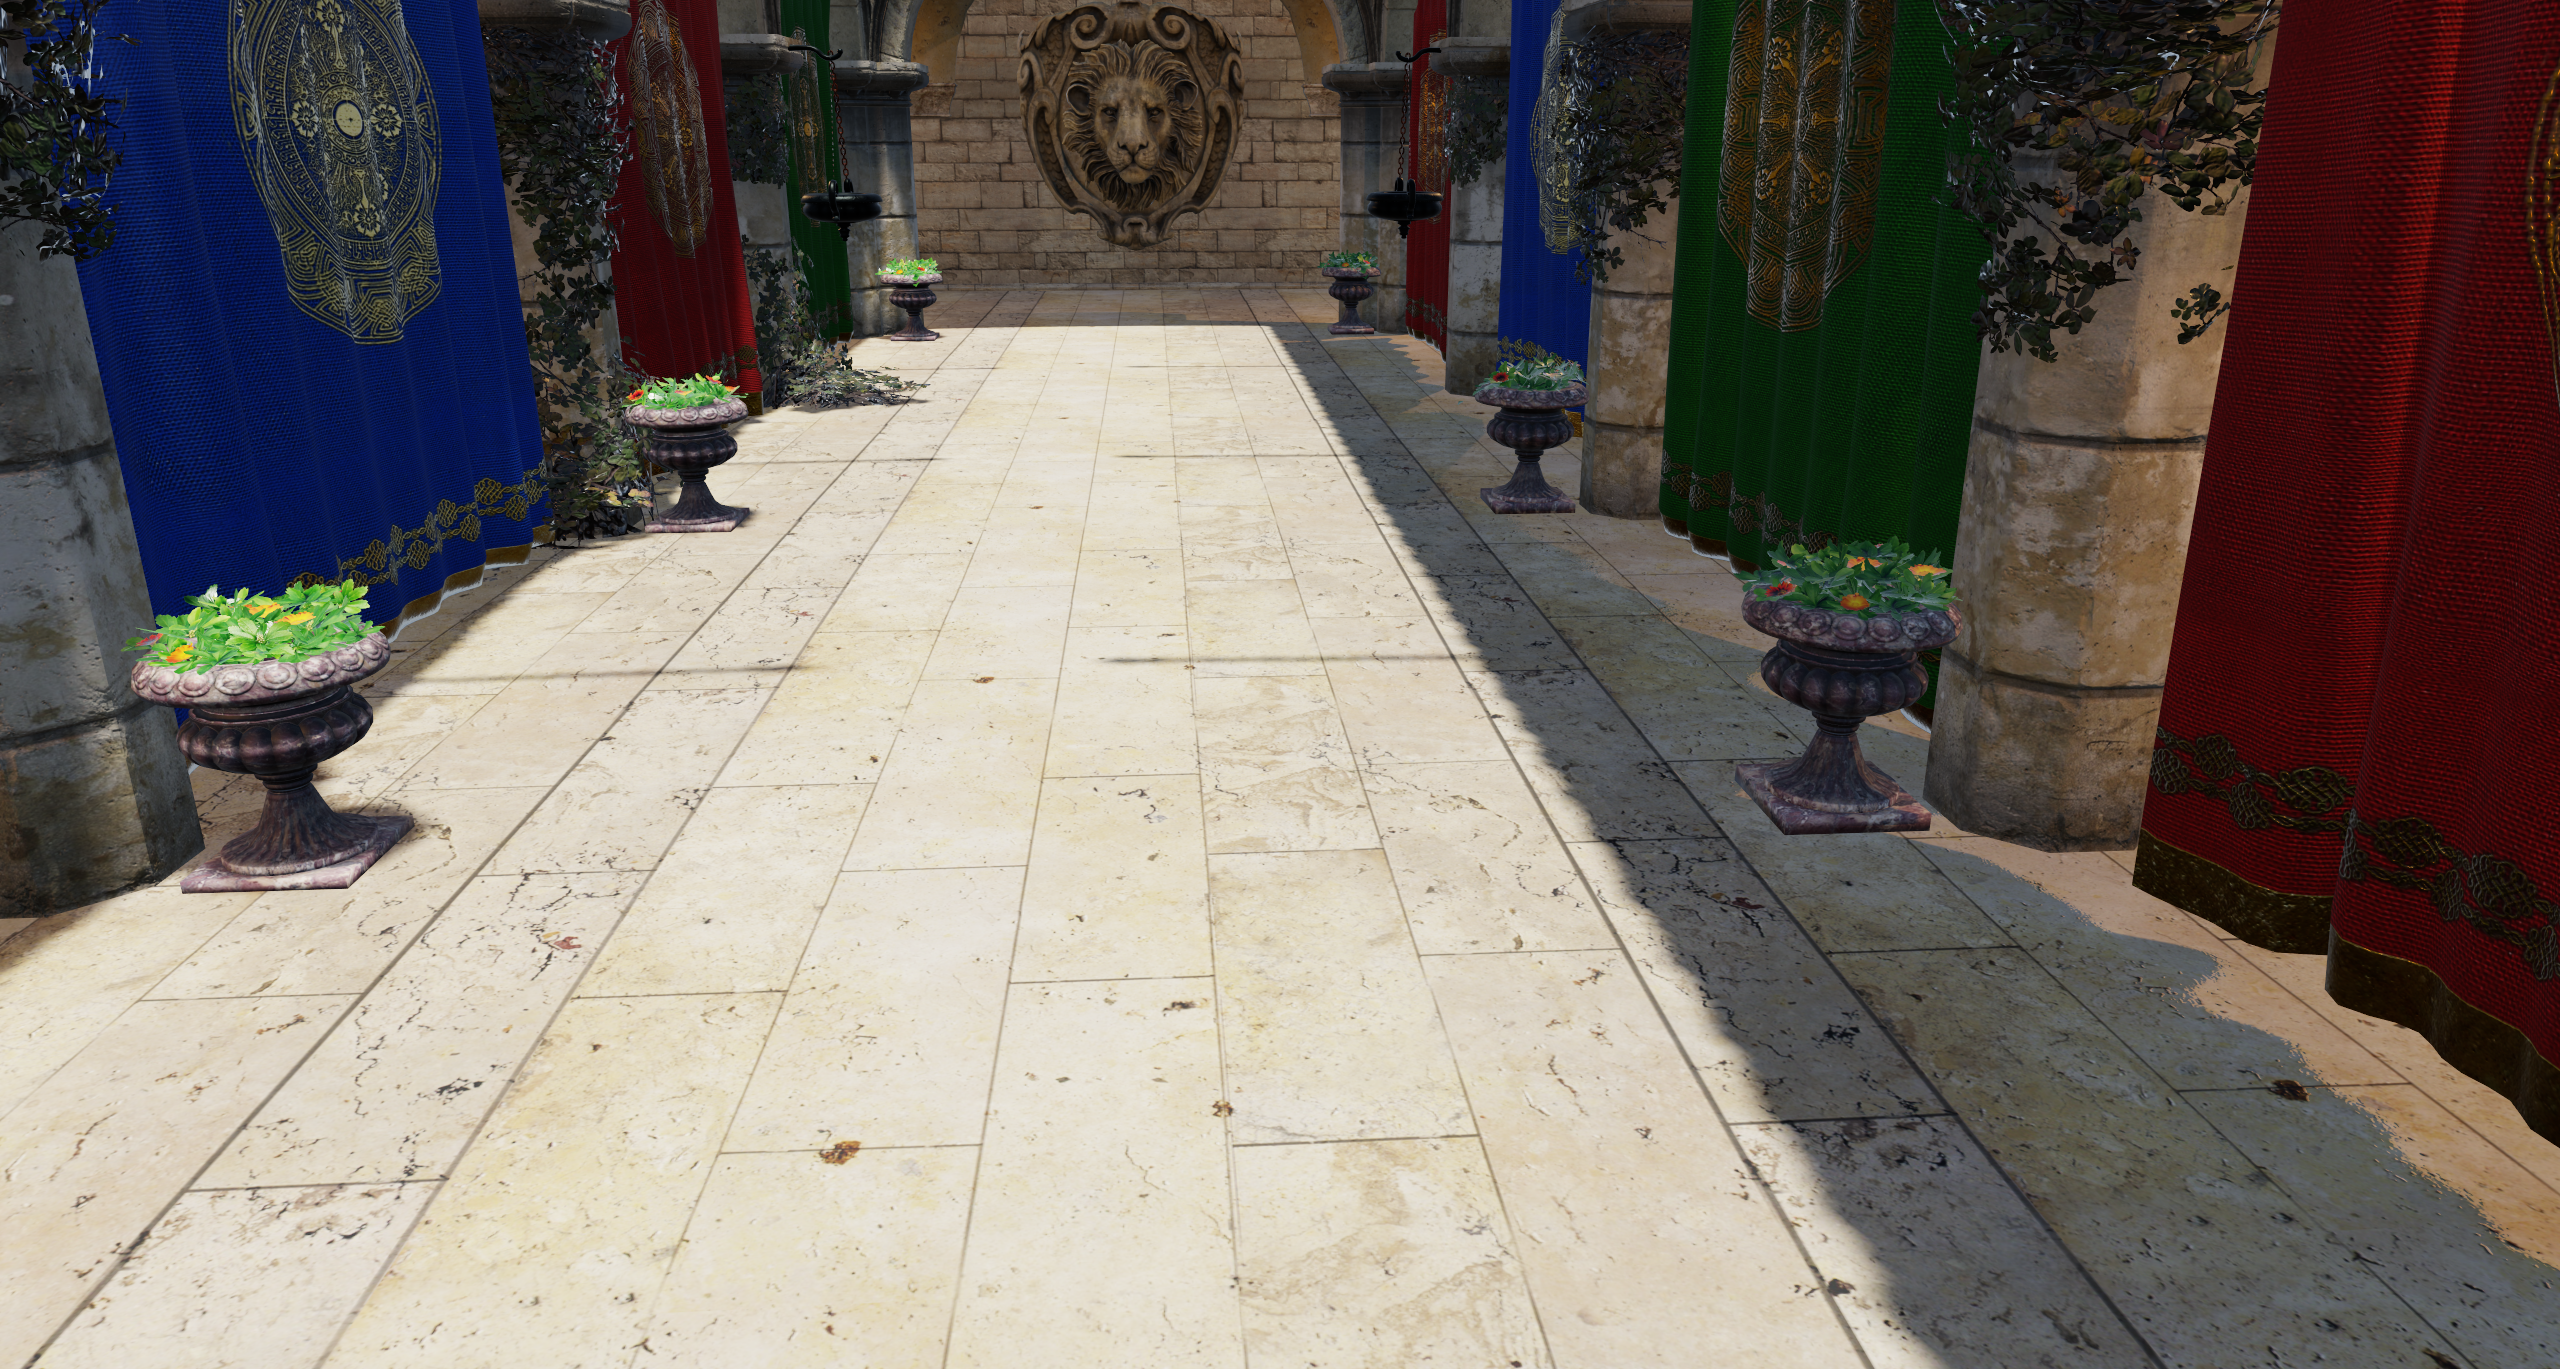
\includegraphics[width=\linewidth]{figures/shadow_map.png}\\{\small mapa senki (raster)}
\end{minipage}\hfill
\begin{minipage}{0.48\textwidth}\centering
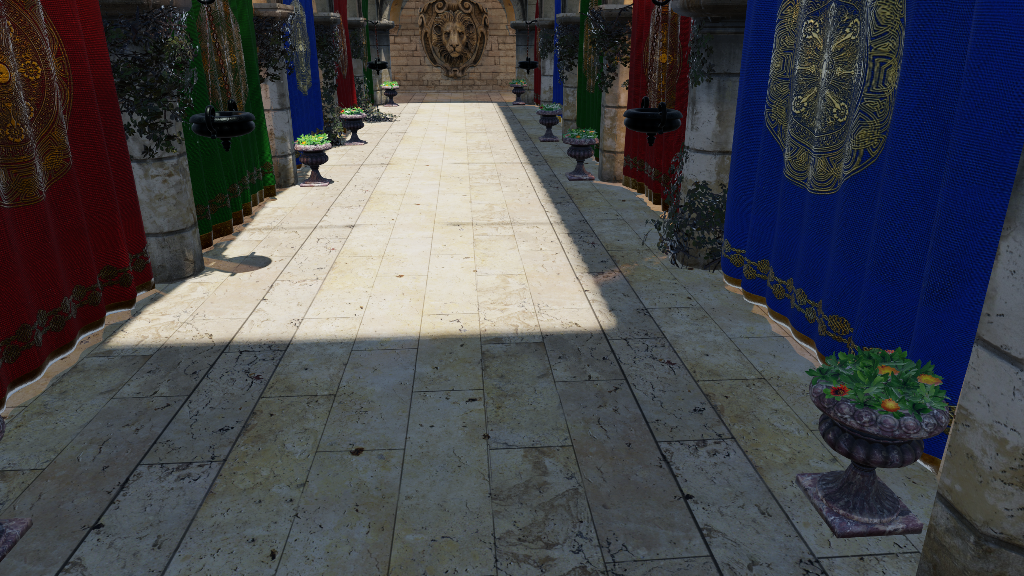
\includegraphics[width=\linewidth]{figures/shadow_rt.png}\\{\small trasirane senke}
\end{minipage}
\caption[Mapa senki naspram trasiranih senki]{Ista poza i isto svetlo, \texttt{render.shadows.mode}
1 naspram 2. Rasterska mapa ima kona\v{c}nu rezoluciju i pomeraj dubine, pa se kontaktne senke
razlivaju i ivice su mek\v{s}e nego \v{s}to geometrija nala\v{z}e, a trasirana verzija ih razre\v{s}ava
preko stvarne geometrije. Snimci su deterministi\v{c}ki (dva uzastopna snimka iste konfiguracije su
identi\v{c}na do bita), pa je svaka razlika izme\dj u panela stvarna.}
\label{fig:shadow-vs-map}
\end{figure}


\needspace{22\baselineskip}
\begin{lstlisting}[caption={Inline ray-query test vidljivosti za senku (HLSL).}, label={lst:shadow}]
RayQuery<RAY_FLAG_ACCEPT_FIRST_HIT_AND_END_SEARCH> q;
RayDesc ray;
ray.Origin    = positionWS + Ng * 0.02 + L * 0.01;
ray.Direction = L;
ray.TMin      = 0.0;
ray.TMax      = distanceToLight - 0.05;   // sun: effectively infinite
q.TraceRayInline(SceneTLAS, RAY_FLAG_NONE, 0xFF, ray);
while (q.Proceed())                       // alpha-test cutout candidates
{
    if (q.CandidateType() == CANDIDATE_NON_OPAQUE_TRIANGLE &&
        RTCommitCandidate(tableAddr, q.CandidateInstanceID(),
                          q.CandidatePrimitiveIndex(),
                          q.CandidateTriangleBarycentrics(), LinearSampler))
    {
        q.CommitNonOpaqueTriangleHit();
    }
}
bool shadowed = (q.CommittedStatus() == COMMITTED_TRIANGLE_HIT);
\end{lstlisting}

Two quality levels are exposed through the \texttt{render.shadow.soft} CVar. The hard path casts one
ray straight at the light, while the soft path casts \texttt{SHADOW_RAY_COUNT = 2} rays sampling, uniformly
by solid angle, the cone the source subtends at the shaded point (Figure~\ref{fig:shadow}), averaging
the hits into a penumbra factor in $[0,1]$. The cone is parameterised by the cosine of its half-angle:
$\cos(\tfrac{1}{2}\,\texttt{render.shadow.sun\_angle\_deg})$ for the sun, and
$\sqrt{1 - (r/d)^2}$ for a local light of radius \texttt{render.shadow.source\_radius} at distance
$d$, so a physically larger or nearer source gives a softer edge. Sampling the solid angle rather
than a tangent-plane disk is what makes the real-time penumbra agree with the path tracer's
next-event estimation at any cone width, instead of only in the small-angle limit where the two
parameterisations coincide. \texttt{SHADOW_RAY_COUNT} is a compile-time constant, a cost class rather
than a live knob. \texttt{render.shadows.rays} applies to the stochastic path below, not to this one.
Directions are decorrelated per pixel and per frame with an interleaved-gradient-noise hash, spreading
the two-sample penumbra across frames for the temporal accumulator to resolve
(Sections~\ref{sec:denoising} and \ref{sec:taa}).

\begin{figure}[tbp]
\centering
\begin{tikzpicture}[>={Stealth[]}]
  \draw[thick] (-2.6,0) -- (2.6,0);                      % surface
  % light-source disk (perpendicular to L), drawn as a circle
  \draw[fill=black!8] (2.7,2.4) circle (0.45);
  \node[font=\scriptsize, align=center] at (2.7,3.25) {izvor\\(polupre\v{c}nik $r$)};
  % direction to the light centre
  \draw[dashed] (0,0) -- (2.7,2.4);
  \node[font=\scriptsize] at (1.55,1.05) {$L$};
  % sample rays fanning to distinct points across the disk
  \draw[->, black!65] (0,0) -- (2.72,2.83);
  \draw[->, black!65] (0,0) -- (3.08,2.22);
  \draw[->, black!65] (0,0) -- (2.36,2.06);
  \draw[<->, black!45] (2.62,2.72) arc (46:38:3.6);
  \node[font=\scriptsize, black!55] at (3.02,2.52) {$\theta/2$};
  \fill (0,0) circle (1.7pt) node[below=3pt] {$P$};
\end{tikzpicture}
\caption{Meke senke: iz ta\v{c}ke $P$ se zraci uzorkuju ravnomerno po prostornom uglu unutar konusa
koji izvor zaklapa oko pravca $L$, sa polovinom ugla $\theta/2$ odre\dj enom polupre\v{c}nikom
izvora $r$ i rastojanjem. Udeo neblokiranih zraka daje penumbru.}
\label{fig:shadow}
\end{figure}

Penumbra width is $2H\tan(\theta/2)$ in the occluder-to-receiver distance $H$ and the source's
angular size $\theta$, so Figure~\ref{fig:shadow-hs} frames the sunlit floor strip: the sun is the
only light here with a distant occluder, its transverse edge cast by the roof light-well lip about
10.4 units above the floor, while the four enabled torches sit a couple of units from the walls they
light. At the sun's true angular diameter that penumbra is roughly 36 pixels of a 2560-wide capture
and disappears once scaled into the page, so the figure raises
\texttt{render.shadow.sun\_angle\_deg} to $3^\circ$ and says so in its caption. Widening
\texttt{render.shadow.source\_radius} instead would be the wrong control, for a reason that is also a
limitation. Cone samples falling below the shading normal's horizon are skipped while the
average still divides by the full sample count, which is deliberate (counting them lit is the leak
that next-event estimation rejects in the path tracer), although it means a wider cone also darkens
grazing surfaces systematically. At a 1.5-unit radius that darkening accounts for about three quarters
of the frame difference and swamps the penumbra it was meant to show. The near-vertical sun meets the
floor at $\mathbf{n}\cdot\boldsymbol{\omega} \approx 1$ and avoids it, since no sample is
horizon-rejected there.

\begin{figure}[tbp]
\centering
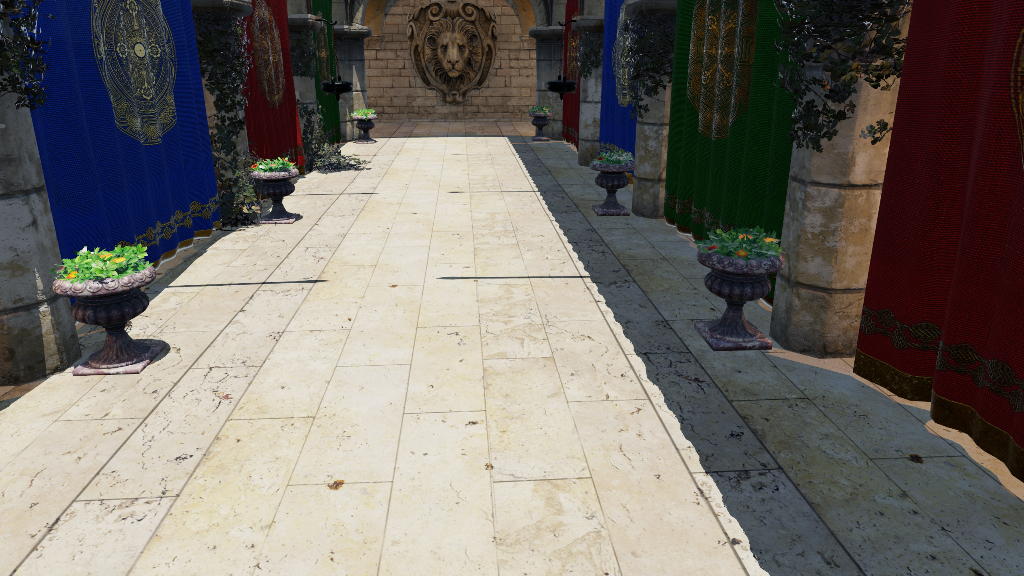
\includegraphics[width=0.48\textwidth]{figures/shadow_hard.png}\hfill%
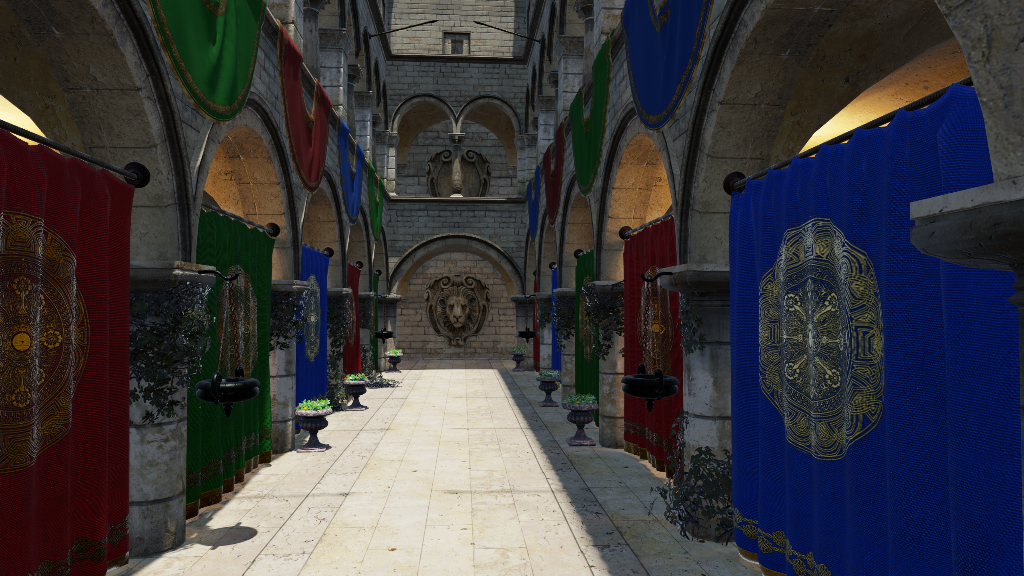
\includegraphics[width=0.48\textwidth]{figures/shadow_soft.png}
\caption{Tvrde (levo) naspram mekih (desno) ray-traced senki na osun\v{c}anoj traci poda: jedina
razlika je \texttt{render.shadow.soft}. Uglovni pre\v{c}nik sunca je podignut na $3^\circ$, oko
\v{s}est puta iznad fizi\v{c}kih $0{,}53^\circ$, jer je na stvarnoj vrednosti penumbra u\v{z}a od
onoga \v{s}to se vidi u \v{s}tampi.}
\label{fig:shadow-hs}
\end{figure}

\paragraph{Stohasti\v{c}ka alternativa.} Tracing one ray per light per pixel is exact but scales
linearly with light count, which does not survive a scene lit by hundreds of sources. The engine
therefore implements a second strategy, enabled by \texttt{render.shadows.stochastic} and off by
default, following the MegaLights approach: each pixel uses resampled importance sampling to pick
\emph{one} light with probability proportional to its unshadowed contribution, traces
\texttt{render.shadows.rays} rays at that light alone, and writes a single aggregate visibility ratio.
The estimate is unbiased but extremely noisy, since one pixel's sample says nothing about which light
its neighbour chose, so this path necessarily runs as its own half-resolution chain,
\texttt{RTShadow} $\rightarrow$ \texttt{ShadowTemporal} $\rightarrow$ \texttt{ShadowDenoise0..2}
$\rightarrow$ \texttt{ShadowUpsample}, reusing the shared denoiser, with a parallel
demodulated-specular chain for the specular occlusion term. Those passes carry their own GPU timestamp
scopes, which Section~\ref{sec:cena} accounts for separately from the forward pass. Its cost is
constant in light count, which is the whole point: the inline path wins for a handful of lights and
loses for many. Section~\ref{sec:analiza-shadow-strategy} measures the crossover on this scene, and
the debug views expose the aggregate visibility buffer before and after filtering
(Figure~\ref{fig:shadow-denoise-ab}), where one sample per pixel is nearly binary noise.

\begin{figure}[tbp]
\centering
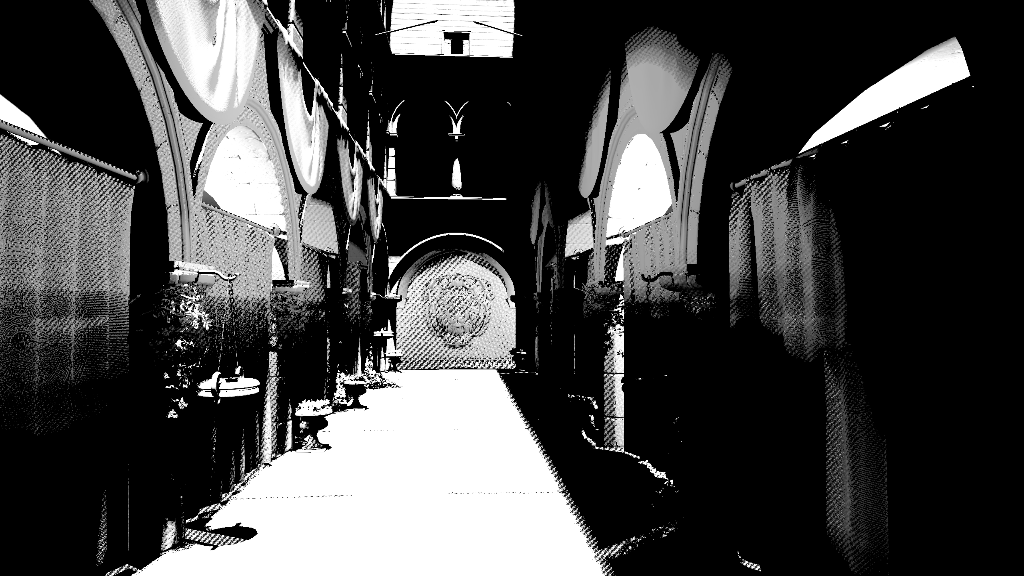
\includegraphics[width=0.48\textwidth]{figures/dbg_shadow_raw.png}\hfill%
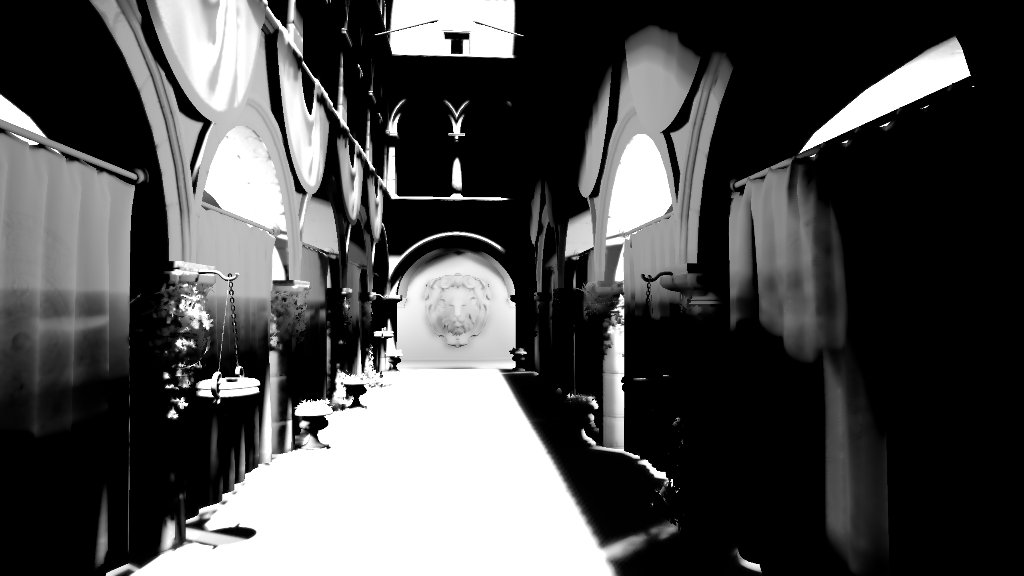
\includegraphics[width=0.48\textwidth]{figures/dbg_shadow_denoised.png}
\caption{Stohasti\v{c}ki agregatni odnos vidljivosti pre (levo) i posle (desno) temporalne
akumulacije i a-trous filtra (\texttt{render.debugview} 8 i 9). Belo je potpuno osvetljeno, crno
potpuno u senci. Levo se vidi da jedan uzorak po pikselu daje skoro binarni \v{s}um.}
\label{fig:shadow-denoise-ab}
\end{figure}

\subsection{Ambijentalna okluzija (AO)}

Ambient occlusion is a compute pass (\texttt{AO.comp.hlsl}) run at half resolution. Each pixel
reconstructs world position from the depth G-buffer and casts \texttt{render.ao.rays} short rays
(default 2, clamped to $[1,16]$) over the cosine-weighted hemisphere around the geometric normal,
rotated per pixel by interleaved gradient noise, using the same
\texttt{ACCEPT_FIRST_HIT_AND_END_SEARCH} visibility traversal as shadows. Rays are limited to
\texttt{render.ao.radius}, and a hit contributes \texttt{1 - saturate(t / AORadius)}, so nearer occluders
darken more, and the result is scaled by \texttt{render.ao.intensity} (Listing~\ref{lst:ao}).


\needspace{17\baselineskip}
\begin{lstlisting}[caption={AO uzorkovanje hemisfere (HLSL, karakteristi\v{c}an ise\v{c}ak).}, label={lst:ao}]
float occlusion = 0.0;
for (uint k = 0; k < RayCount; ++k)
{
    float3 dir = CosineHemisphere(k, RayCount, ign, N); // cosine-weighted, IGN-rotated around N
    RayQuery<RAY_FLAG_ACCEPT_FIRST_HIT_AND_END_SEARCH> q;
    RayDesc ray = MakeRay(positionWS + N * 0.02, dir, 0.0, AORadius);
    q.TraceRayInline(SceneTLAS, RAY_FLAG_NONE, 0xFF, ray);
    while (q.Proceed()) { /* alpha-test cutout candidates, as in Listing 3.1 */ }
    if (q.CommittedStatus() == COMMITTED_TRIANGLE_HIT)
        occlusion += 1.0 - saturate(q.CommittedRayT() / AORadius);
}
occlusion = 1.0 - occlusion / RayCount;
\end{lstlisting}

The pass writes \texttt{float4(ao, ao, ao, meanHitT)}, the alpha channel carrying the mean
distance to the occluders. That alpha feeds a hit-distance-guided edge-stopping term in the
denoiser (Section~\ref{sec:denoising}), the same idea NVIDIA's ReBLUR denoiser \cite{nvidia_nrd} uses
to scale the spatial filter by how far the occluder was. The term is implemented but disabled by
default on every signal, AO included: at two rays per pixel the hit distance is itself too noisy to
steer the filter, and a wrong steer is worse than none. The half-resolution result is denoised and
bilaterally upsampled before the forward pass multiplies it into the ambient term
(Figure~\ref{fig:ao}).

\begin{figure}[tbp]
\centering
\begin{tikzpicture}[>={Stealth[]}]
  \draw[thick] (-2.7,0) -- (2.7,0);
  \draw[dashed] (-1.9,0) arc (180:0:1.9);
  \draw[->, thick] (0,0) -- (0,2.25) node[above] {$N$};
  \foreach \a in {30,60,90,120,150} \draw[->, black!60] (0,0) -- (\a:1.9);
  \draw[fill=black!12] (0.85,0.55) rectangle (1.3,1.25);
  \draw[thin] (1.3,1.1) -- (2.05,1.6);
  \node[font=\scriptsize, anchor=west] at (2.05,1.6) {okluder};
  \fill (0,0) circle (1.7pt) node[below=3pt] {$P$};
\end{tikzpicture}
\caption{Uzorkovanje po hemisferi za AO: iz ta\v{c}ke $P$ se baca vi\v{s}e kratkih zraka po hemisferi
oko normale $N$. Udeo zraka koji u zadatom polupre\v{c}niku pogodi geometriju daje okluziju.}
\label{fig:ao}
\end{figure}

\subsection{Refleksije (reflections)}

Reflections are a compute pass (\texttt{Reflection.comp.hlsl}) run at full resolution, the only
ray-traced effect not traced at half res, since reflection detail is view-dependent and does not
tolerate the blur that half-res tracing plus upsampling introduces. Each pixel reconstructs world
position and reflects the view vector about the normal-mapped shading normal (read from a separate
shading-normal G-buffer, not the geometric normal, so normal maps are mirrored correctly). It needs
the closest hit, so unlike the visibility queries it uses a plain \texttt{RayQuery<RAY_FLAG_NONE>}
and runs traversal to completion.

Glossy reflections are approximated by jittering each ray inside a cone whose half-angle scales with
surface roughness (\texttt{roughness * ReflConeScale}), averaged over \texttt{render.reflections.rays}
(default 1), while a mirror surface (\texttt{roughness == 0}) collapses to one sharp ray. Hits are
shaded by \texttt{ShadeSurfaceHit} (sun lighting with its own shadow ray, the hit surface's emissive
term, image-based ambient), and a miss samples the prefiltered sky cube. Unlike the GI pass below, reflections
do not sample the scene's local point and spot lights at the hit: the same importance-sampled
local-light estimator was measured here too and showed no quality gain for twice the GI side's cost,
so it is compiled out of this pass entirely. The pass writes raw reflected radiance plus hit distance,
while the Fresnel term, the BRDF weighting, and \texttt{render.reflections.intensity} are applied
afterward in the forward pass (Figure~\ref{fig:refl}).

\begin{figure}[tbp]
\centering
\begin{tikzpicture}[>={Stealth[]}]
  \draw[thick] (-2.7,0) -- (2.7,0);
  \draw[->, thick] (0,0) -- (0,2.2) node[above] {$N$};
  \draw[->, black!55] (-2.05,2.05) -- (0,0); \node[font=\scriptsize] at (-1.55,1.35) {$V$};
  \foreach \a in {50,62,74} \draw[->, black!65] (0,0) -- (\a:2.15);
  \draw[dashed] (0,0) -- (62:2.3) node[above right, font=\scriptsize] {$R$};
  \node[font=\scriptsize, align=center] at (2.0,1.05) {konus\\(hrapavost)};
  \fill (0,0) circle (1.7pt) node[below=3pt] {$P$};
\end{tikzpicture}
\caption{Refleksije: pravac odbijanja $R$ vektora pogleda $V$ oko normale $N$. Glatka povr\v{s}ina
daje jedan o\v{s}tar zrak, a hrapava uzorkuje konus oko $R$.}
\label{fig:refl}
\end{figure}

Figure~\ref{fig:refl-onoff} shows the contribution of the pass. The cone itself
(Figure~\ref{fig:refl-cone}) resists the obvious measurement: sweeping
\texttt{render.reflections.cone\_scale} from 0 (a pure mirror ray) to 3 changes the finished frame by
a mean of only 0.16 levels out of 255, across six camera poses tried. The cause is that the reflection
is a small additive term next to direct lighting, so the composited image hides it. Measured on the
reflection buffer before compositing, the same A/B moves 43.7 levels and drops the buffer's
high-frequency energy from \hfConeSharp{} to \hfConeGlossy{}, a factor of 275 more signal than the
composited comparison shows. The figure therefore uses the isolated buffer, for the same reason the
effect gallery in Section~\ref{sec:cena} does: a term that is small in the final image can still be
the whole content of its own intermediate.

\begin{figure}[tbp]
\centering
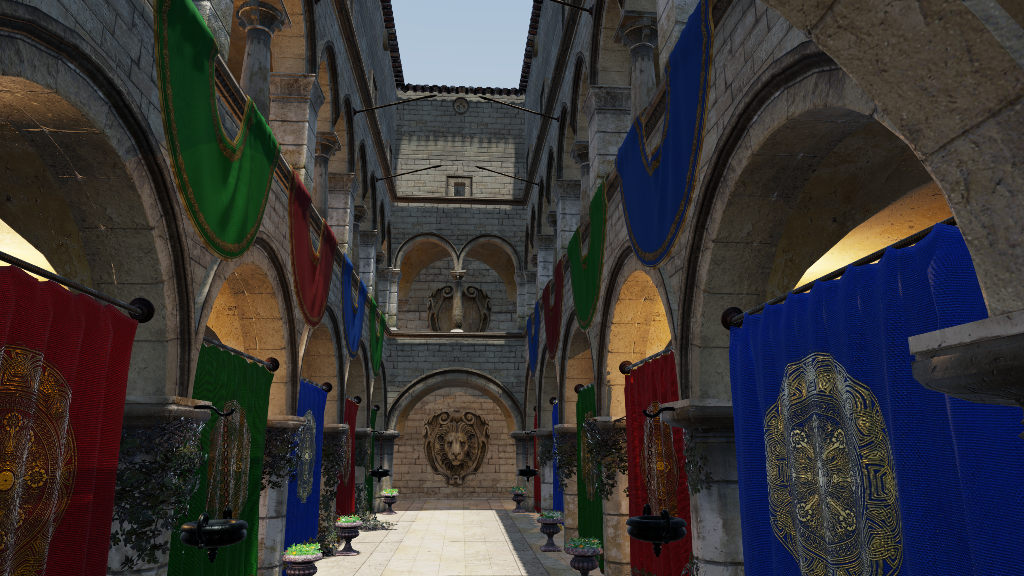
\includegraphics[width=0.48\textwidth]{figures/refl_off.png}\hfill%
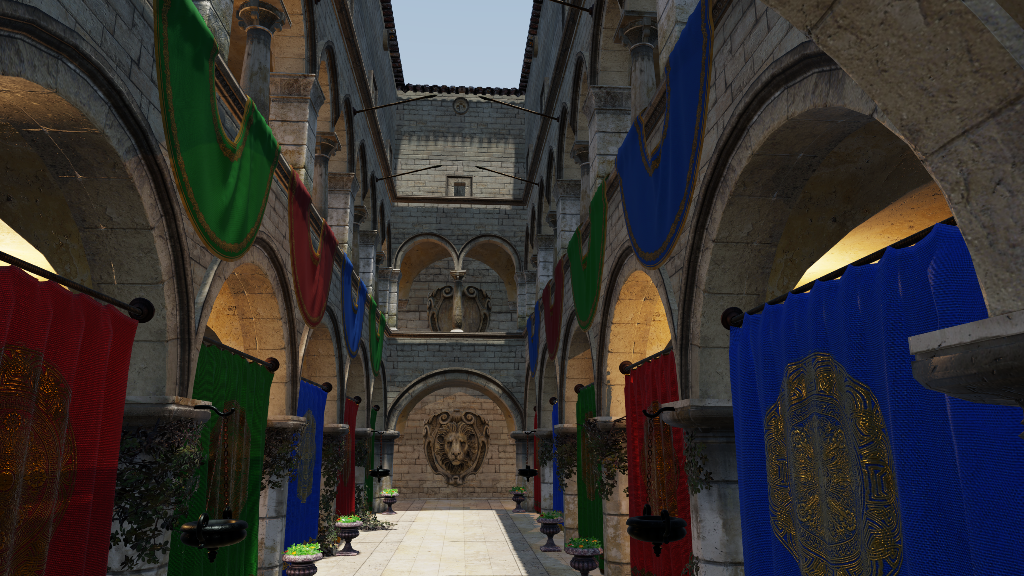
\includegraphics[width=0.48\textwidth]{figures/refl_rt.png}
\caption{Bez refleksija (levo) naspram ray-traced refleksija (desno), pri uglu gledanja blizu
tangentnog gde je Fresnel-ov doprinos najve\'ci. Sjaj na draperijama i kamenu je razlika koju
donosi prolaz.}
\label{fig:refl-onoff}
\end{figure}

\begin{figure}[tbp]
\centering
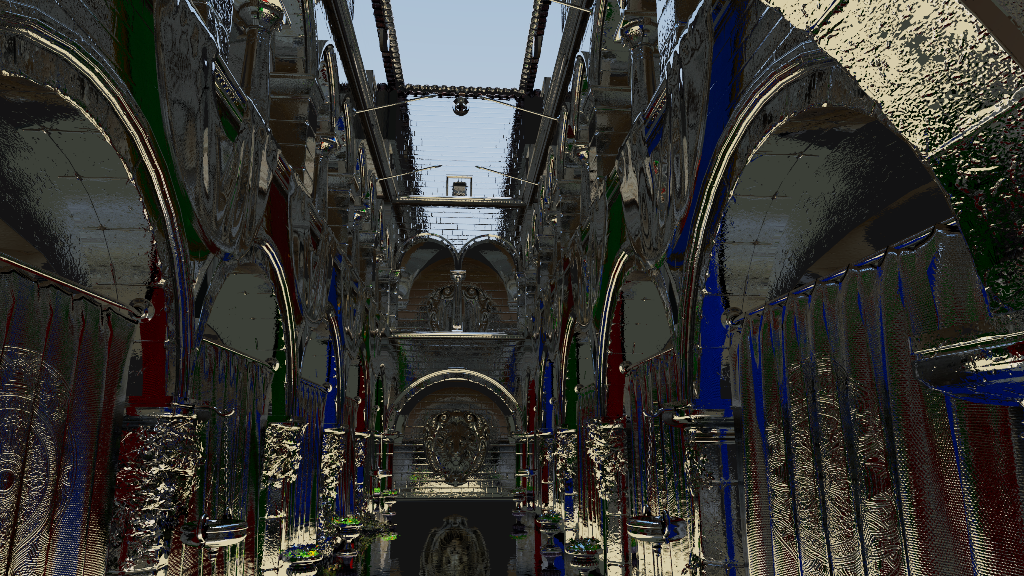
\includegraphics[width=0.48\textwidth]{figures/cone_sharp.png}\hfill%
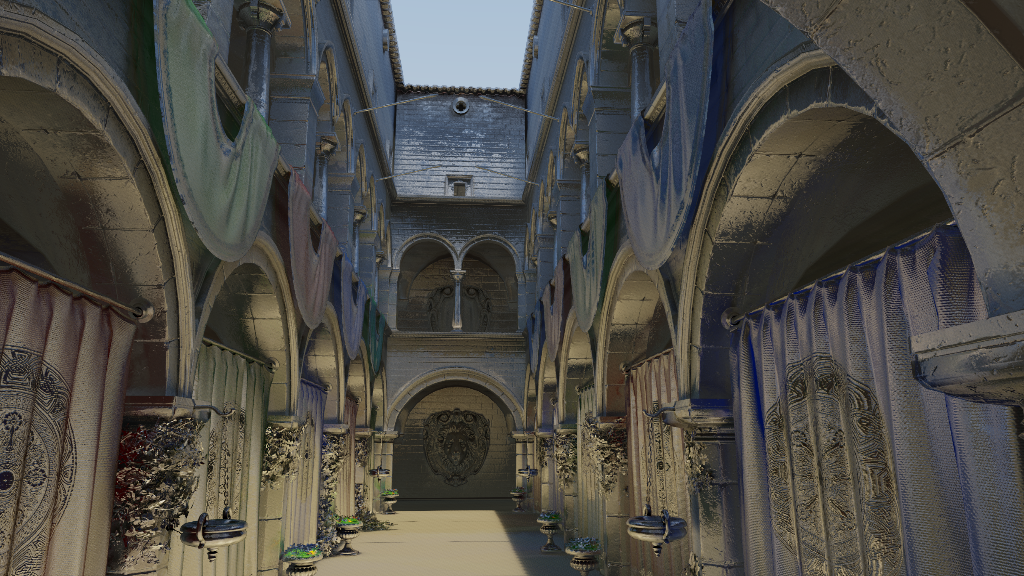
\includegraphics[width=0.48\textwidth]{figures/cone_glossy.png}
\caption{Reflektovana radijansa pre kombinovanja (\texttt{render.debugview} 3): o\v{s}tar ogledalski
zrak, \texttt{cone\_scale} 0 (levo), naspram konusa \v{s}irenog hrapavo\v{s}\'cu, \texttt{cone\_scale}
3 (desno). U gotovoj slici se ova razlika ne vidi jer je refleksija mali aditivni \v{c}lan pored
direktnog osvetljenja, a u sopstvenom baferu ona je ceo sadr\v{z}aj.}
\label{fig:refl-cone}
\end{figure}

\subsection{Globalno osvetljenje (GI)}

Global illumination is the most expensive effect: a compute pass (\texttt{GI.comp.hlsl}) run at half
resolution that computes one bounce of diffuse indirect light. It samples the hemisphere exactly as
AO does, \texttt{render.gi.rays} rays (default 2) out to \texttt{render.gi.range}. The difference is
what a ray returns. A miss samples the sky cube, and each hit is shaded by
\texttt{ShadeSurfaceHit}: the sun with its own shadow ray,
the hit surface's emissive term, an image-based ambient fill, and, when \texttt{render.rt.hit_lights}
is on (the default), one of the scene's point and spot lights. That light is importance-sampled in
proportion to its unshadowed contribution at the hit and confirmed with its own shadow ray, an
unbiased single-sample estimator (the same one \texttt{RTShadowPass} uses, in the spirit of UE5's
MegaLights) whose cost is constant in the light count, unlike a full next-event-estimation sum over
every light, which would multiply the ray budget at every secondary hit. This term is GI-only, and the
routine does not re-trace beyond these shadow rays, so the evaluation remains one bounce.

The pass outputs incoming irradiance only, without the receiver's albedo, which is multiplied in at
full resolution in the forward pass. This is the demodulated-irradiance convention that both the SVGF
denoiser and probe systems such as DDGI/RTXGI \cite{majercik2019ddgi, nvidia_rtxgi} rely on: filtering
irradiance rather than final color keeps the denoiser's edge-stopping from being misled by albedo
texture detail. The forward pass then replaces its flat ambient term with this ray-traced indirect,
the same substitution Lumen and RTXGI make \cite{epic_lumen}. At two rays per pixel and half
resolution (Figure~\ref{fig:gi}) the raw output is usable only after the temporal-plus-spatial denoise
of Section~\ref{sec:denoising}.

\begin{figure}[tbp]
\centering
\begin{tikzpicture}[>={Stealth[]}]
  \draw[thick] (-2.9,0) -- (2.9,0);
  \draw[dashed] (-2.1,0) arc (180:0:2.1);
  \draw[->, thick] (0,0) -- (0,2.45) node[above] {$N$};
  \foreach \a in {35,70,110,145} \draw[->, black!60] (0,0) -- (\a:2.1);
  \foreach \a in {35,70,110,145} \fill[black!30] (\a:2.1) circle (2.4pt);
  \fill (0,0) circle (1.7pt) node[below=3pt] {$P$};
\end{tikzpicture}
\caption{Globalno osvetljenje: kosinusno uzorkovanje hemisfere oko $N$ iz ta\v{c}ke $P$. Svaki zrak
koji pogodi geometriju vra\'ca radijansu (jedno odbijanje).}
\label{fig:gi}
\end{figure}

Figure~\ref{fig:gi-onoff} shows the scene without and with ray-traced global illumination.

\begin{figure}[tbp]
\centering
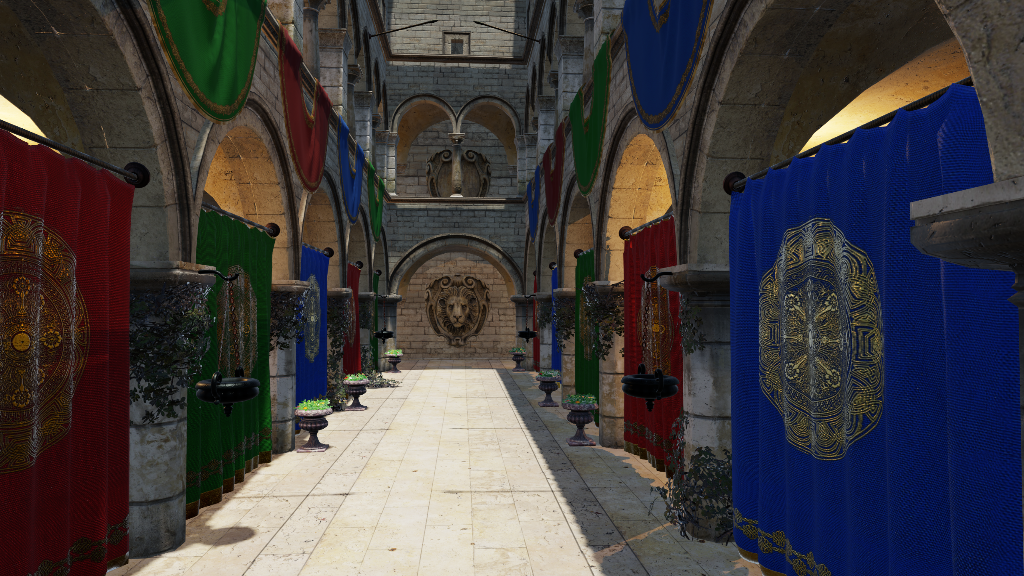
\includegraphics[width=0.82\textwidth]{figures/gi_off.png}

\vspace{6pt}

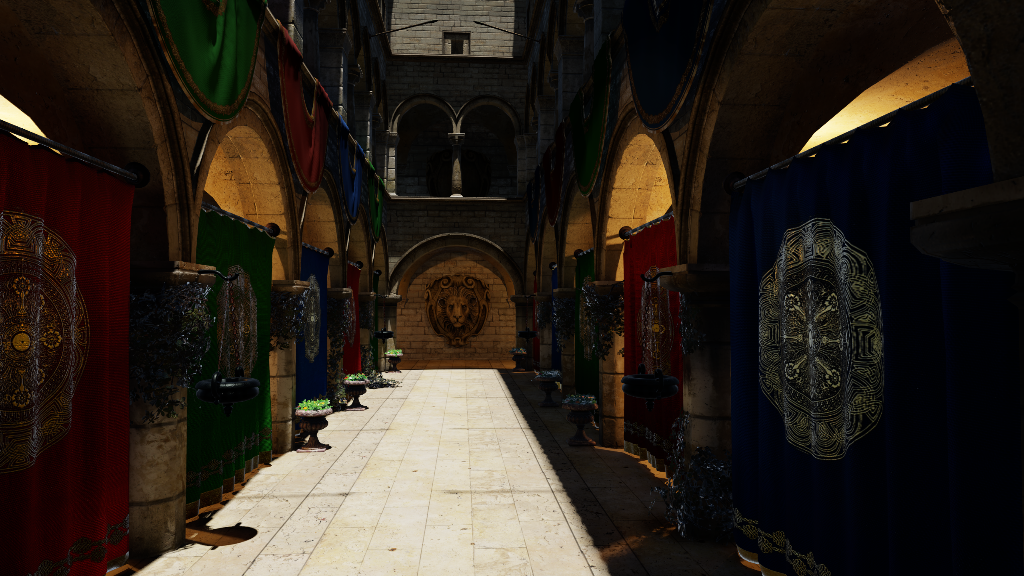
\includegraphics[width=0.82\textwidth]{figures/gi_on.png}
\caption{Scena bez (gore) i sa (dole) globalnim osvetljenjem: jedan difuzni indirektni odboj daje
prelivanje boja i popunu u senkama.}
\label{fig:gi-onoff}
\end{figure}

\section{Denoising (SVGF)}
\label{sec:denoising}

Each effect here estimates an integral over incoming directions from one or two samples, and
$\sqrt{n}$ convergence means samples alone cannot buy a clean image inside a frame budget. The
missing samples do exist, just not in this pixel and this frame: neighbouring pixels usually look at
nearly the same surface, and the previous frame usually contains the same surface one small camera
motion away. A denoiser borrows those samples spatially and temporally while refusing to borrow
across a real edge, where the neighbour is a different surface and averaging would smear the image.
Deciding what counts as "the same surface" is the entire difficulty, and it is why a denoiser needs
the G-buffer's depth and normals rather than just the colour.

Snowstorm implements a variant of Spatiotemporal Variance-Guided Filtering (SVGF)
\cite{schied2017svgf}, the standard real-time reconstruction filter for path-traced effects, as a
single signal-agnostic component. One \texttt{Denoiser} class (\texttt{Render/Denoiser.\{hpp,cpp\}})
drives a temporal accumulation and a spatial \`a-trous filter, with all per-viewport GPU state
(history, moments, scratch ping-pong textures) in a \texttt{DenoiserInstance} component the caller
owns. It is instantiated four times, for shadows, GI, AO, and reflections, each with its own
configuration but identical code (Figure~\ref{fig:svgf}). The reuse is possible because the noisy
estimate, its variance inputs, and the depth/normal G-buffer are the only signal-specific data. The
hit-distance
edge-stopping weight is wired up for every signal but left at zero by default, so that term is a
no-op in the measured configuration. The stochastic shadow path instead sizes its kernel by occluder
distance directly, in the NRD SIGMA style, through \texttt{render.shadows.denoise.penumbra}.
Reflections reuse GI's temporal shader, a limitation since a reflection history has view-dependent
content that a diffuse-tuned reprojection does not perfectly handle.

\begin{figure}[tbp]
\centering
\begin{tikzpicture}[>={Stealth[]}, node distance=5mm,
  box/.style={draw, rounded corners, align=center, text width=10.6cm, inner sep=4pt, font=\small}]
  \node[box] (in)  {Noisy input (GI and AO at half resolution, reflections at full)};
  \node[box, below=of in]  (tp) {\textbf{Temporal:} reproject by motion vectors, accumulate history
    (up to 32 frames), estimate per-pixel variance};
  \node[box, below=of tp]  (at) {\textbf{\`A-trous spatial filter:} 3 iterations by default (up to 5),
    stride $1, 2, 4, \dots$; edge-stopping on normal, depth, and variance};
  \node[box, below=of at]  (out){Denoised, then upsampled, into the Forward pass};
  \draw[->] (in) -- (tp); \draw[->] (tp) -- (at); \draw[->] (at) -- (out);
\end{tikzpicture}
\caption{SVGF denoiser: temporalna akumulacija sa procenom varijanse, zatim varijansom-vo\dj en
\`a-trous prostorni filter, deljen izme\dj u GI, AO i refleksija.}
\label{fig:svgf}
\end{figure}

\subsection{Temporalna akumulacija}

The temporal pass (\texttt{GITemporal.comp.hlsl}, at trace resolution) reprojects the previous
frame's result by the motion vectors (\texttt{prev_uv = uv - velocity}) and blends it with the
current noisy input. Off-screen samples and the first frame reset to the current input, and a
relative-depth test rejects disoccluded pixels. The blend follows SVGF's history-length scheme: a
per-pixel accumulated history length, capped at 32 frames, sets the blend weight
\texttt{max(alphaMin, 1 / historyLength)}, so a freshly disoccluded pixel weights the current frame
heavily while a long-lived pixel averages many frames. First and second luminance moments accumulate
with the same weight, and their difference is the temporal variance that guides the spatial filter.
Pixels too young for a stable temporal variance (history under four frames) fall back to a
$7\times7$ spatial variance estimate.

A neighborhood color clamp is added over stock SVGF: the reprojected history is clipped toward the
mean of a $3\times3$ current-frame neighborhood, weakened when the pixel is static and tightened when
it moves. This TAA-style clamp suppresses ghosting on moving edges and in reflections, where
depth/normal rejection alone is insufficient.

\subsection{Prostorni \`a-trous filter}

The spatial pass (\texttt{GIDenoise.comp.hlsl}) is the \`a-trous wavelet filter at the core of SVGF:
each iteration is a $5\times5$ tap gather with a B3-spline kernel, and successive iterations double
the tap stride (\texttt{step = 1 << i}). The engine runs up to five iterations, configurable per
signal. At the default three (Figure~\ref{fig:atrous}) the cumulative reach is $2(1+2+4) = 14$ texels,
a $29\times29$ support gathered with $75$ taps instead of the $841$ a dense gather would cost. The
holes pay for the reach, and the edge-stopping weights keep the widening passes from leaking across
geometry.

\begin{figure}[tbp]
\centering
\begin{tikzpicture}[font=\scriptsize, scale=0.2]
  \foreach \it/\stride/\xoff in {0/1/0, 1/2/22, 2/4/44} {
    \begin{scope}[xshift=\xoff cm]
      \draw[black!15] (-8.5,-8.5) grid (8.5,8.5);
      \foreach \dy in {-2,-1,0,1,2} \foreach \dx in {-2,-1,0,1,2} {
        \pgfmathsetmacro{\px}{\dx*\stride}
        \pgfmathsetmacro{\py}{\dy*\stride}
        \fill[black!62] (\px-0.5,\py-0.5) rectangle (\px+0.5,\py+0.5);
      }
      \fill[white] (-0.5,-0.5) rectangle (0.5,0.5);
      \draw[black, thick] (-0.5,-0.5) rectangle (0.5,0.5);
      \node[font=\small] at (0,-10.4) {iteracija \it, korak \stride};
      \node[font=\small] at (0,-12.6) {doseg $\pgfmathparse{int(4*\stride+1)}\pgfmathresult
        \times \pgfmathparse{int(4*\stride+1)}\pgfmathresult$};
    \end{scope}
  }
\end{tikzpicture}
\caption[\`A-trous: rastu\'ci korak i doseg filtra]{Tri iteracije a-trous filtra, sve nad istim
$17\times17$ isecem oko piksela koji se filtrira (beli kvadrat u sredini). Svaka iteracija uzima
istih 25 uzoraka, samo sa dvostruko ve\'cim korakom, pa doseg raste a cena po iteraciji ostaje ista.
Rupe izme\dj u uzoraka su ono \v{c}ime se pla\'ca doseg: kumulativno $29\times29$ za 75 uzoraka
umesto 841.}
\label{fig:atrous}
\end{figure}

Each tap carries three edge-stopping terms (Listing~\ref{lst:atrous}): normal, relative linearized
depth, and the variance-guided luminance term that is the defining idea of SVGF. Because the
luminance weight scales with the square root of the filtered variance, the filter blurs aggressively
where the signal is noisy and preserves detail where it has converged. Variance itself is filtered
with the squared tap weights, and all guide buffers are point-sampled to avoid bleeding across edges.
Disabling the variance term (\texttt{LumaPhi = 0}) reduces the filter to a plain bilateral blur, a
useful baseline in Chapter~\ref{ch:analiza}.


\needspace{12\baselineskip}
\begin{lstlisting}[caption={Edge-stopping te\v{z}ine za \`a-trous filter (SVGF jezgro, HLSL).}, label={lst:atrous}]
float w_n = pow(saturate(dot(N, N_tap)), K_NORMAL);              // normal
float w_z = exp(-abs(z - z_tap) / (K_DEPTH * abs(dzdx) + 1e-4)); // depth
float w_l = exp(-abs(lum - lum_tap) /                            // variance-guided luminance
                (LUMA_PHI * sqrt(varBlur) + 1e-4));
float w   = w_n * w_z * w_l * kernel[dy + 2] * kernel[dx + 2];   // combined tap weight
sum  += w * color_tap;
wSum += w;
\end{lstlisting}

\subsection{Odstupanja od SVGF i cena}

The implementation departs from the paper in a few places, all noted so Chapter~\ref{ch:analiza}'s
quality numbers are read correctly: the denoiser filters raw irradiance and remultiplies albedo after
upsampling rather than demodulating inside the filter as SVGF does; the extra temporal color clamp
above is not in SVGF; GI and AO are filtered at half resolution where SVGF is full-resolution; and
the variance edge-stop is optional. \texttt{GIDenoise.comp} keeps its outer à-trous loop rolled rather
than unrolled, which costs a little scheduling freedom and in exchange holds register pressure down to
70 VGPRs on the RX 7900 XTX and 59 on the RX 9070 XT, with no spilling and full occupancy on both
(Table~\ref{tab:occupancy}). Unrolled it allocates 191 and drops to 8 of 16 wavefronts.

\section{TAA / temporal resolve}
\label{sec:taa}

After the forward pass produces the shaded HDR image, a temporal anti-aliasing resolve \cite{karis2014taa}
(\texttt{TemporalResolvePass}, \texttt{TemporalResolve.frag.hlsl}) accumulates it across frames to
remove aliasing and to converge the residual noise the per-effect denoisers leave behind. The camera
projection is jittered every frame by a Halton(2,3) sequence over a 16-phase cycle. The resolve
reprojects the previous output by the motion vectors (with a closest-depth dilation so thin features
fetch the right velocity), reconstructs the history with a Catmull-Rom filter to reduce reprojection
blur, and clips it against the current $3\times3$ neighborhood in YCoCg space using a Karis
rounded-box bound, loosened for static pixels and tightened under motion.

The resolve runs in linear HDR and does accumulation only. This is a deliberate invariant: any
perceptual or display-space operation (sharpening, contrast) is kept out of this pass and applied
after tonemap, since a per-channel curve applied before tonemap turns an accumulation overshoot into
a hue shift. Sharpening therefore lives in a separate post-tonemap pass, not here.

Motion vectors are the shared prerequisite of three consumers: the SVGF temporal pass, the TAA
resolve, and the screen-space effects that gather last frame's colour. The velocity pass
(Figure~\ref{fig:motion}) renders the scene a second time and writes per pixel the screen-space
displacement of a surface point between the previous and current view-projection matrices.

The failure mode this exposes is disocclusion. A pixel revealed from behind an occluder this frame
has no previous position to point at, so its history is meaningless and reusing it would smear the
occluder's colour across the newly visible surface. Every temporal stage in the engine therefore
pairs the reprojection with a rejection test on depth and normal, and where that test fires the pixel
falls back to the current frame alone, which is noisier but correct.

\begin{figure}[tbp]
\centering
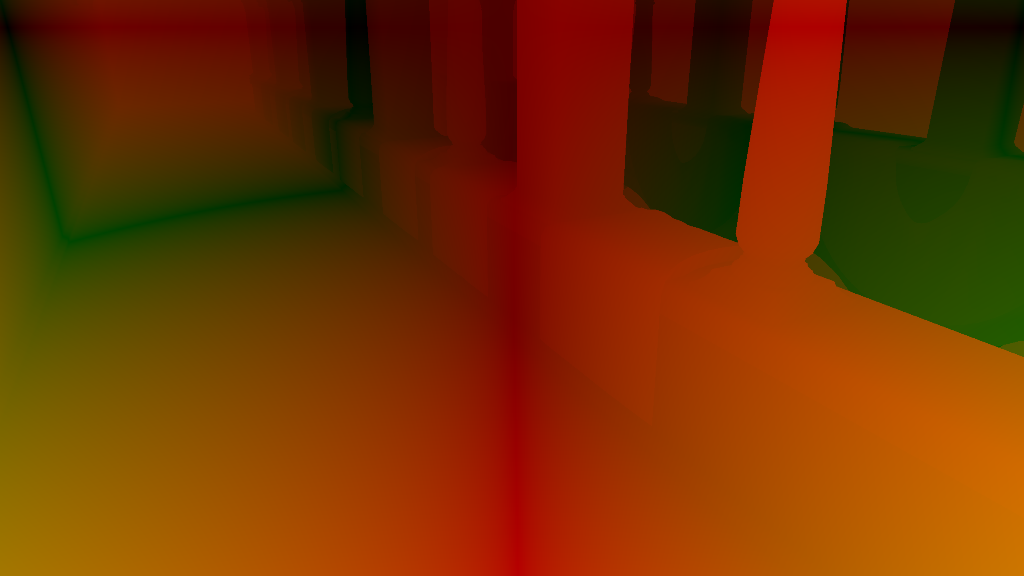
\includegraphics[width=0.8\textwidth]{figures/dbg_motion.png}
\caption{Bafer vektora kretanja (\texttt{render.debugview} 1) tokom determinis\-ti\v{c}ke orbite
kamere. Crveno je vodoravna, zeleno uspravna komponenta pomeraja piksela izme\dj u dva uzastopna
kadra. Prikaz uzima apsolutnu vrednost i mno\v{z}i je sa 40, pa se vidi \emph{koliko} se piksel
pomera i po kojoj osi, ali ne i u kom smeru. Crno je izostanak pomeraja, ali i nebo, koje kroz ovaj
prolaz uop\v{s}te ne upisuje vektore. Prikaz nije kalibrisan: kanali su normirani po \v{s}irini
odnosno visini, pa im osvetljenost nije na istoj skali, a izlaz je jo\v{s} i sRGB kodiran. Kada se
to poni\v{s}ti, prose\v{c}an pomeraj u ovom kadru je oko $0{,}6\%$ dijagonale ekrana po kadru,
najvi\v{s}e $1{,}6\%$, i nijedan uzorak nije zasi\'cen.}
\label{fig:motion}
\end{figure}

\section{Reproducibilnost i alati}
\label{sec:alati}

The measurements in Chapter~\ref{ch:analiza} come from instrumentation built into the engine, which
is what makes them reproducible rather than one-off captures. Every effect is toggled and tuned
through a console-variable registry, so a benchmark configuration is a set of CVar values rather than
a code change, settable from the command line for headless runs, and each render-graph pass is
bracketed by a GPU timestamp scope. Four of the harnesses built on top (Table~\ref{tab:tooling})
compare against a committed baseline and fail the run on a regression, which is what separates a gate
from a report: a number nobody checks drifts.

\begin{table}[tbp]
\caption[Merni alati]{Alati koji proizvode brojeve iz Glave~\ref{ch:analiza}. ,,Kapija`` zna\v{c}i da
alat pore\dj uje sa committovanim baseline-om i obara izvr\v{s}avanje pri regresiji, a alati bez
kapije samo izve\v{s}tavaju. Svi osim \texttt{rga-occupancy} zahtevaju stvarni GPU, pa se izvr\v{s}avaju
lokalno, ne na CI-u.}
\label{tab:tooling}
\centering
\begin{tabular}{lll}
\toprule
Alat & \v{S}ta meri & Kapija \\
\midrule
\texttt{perf-bench}     & GPU ms po prolazu, matrica konfiguracija & da \\
\texttt{quality-bench}  & FLIP/PSNR/SSIM naspram path trace-a, stati\v{c}na kamera & da \\
\texttt{quality-motion} & FLIP, tFLIP, ka\v{s}njenje i JOD du\v{z} rute & da \\
\texttt{rga-occupancy}  & registarski pritisak i zauzetost, offline & da \\
\texttt{quality-tune}   & pretraga CVar-ova prema referenci & ne \\
\texttt{smoke-test}     & pad, zaglavljivanje, Vulkan validacija & pass/fail \\
\texttt{shader-stats}   & registri iz drajvera, oba proizvo\dj a\v{c}a & ne \\
Tracy + watchdog        & vremenska linija po sistemu, zastoji po frejmu & ne \\
\bottomrule
\end{tabular}
\end{table}

\section{Referentni path tracer}
\label{sec:pathtracer}

The reference is a brute-force unidirectional path tracer built into the engine
(\texttt{PathTrace.comp.hlsl}): next-event estimation to the sun, the same metallic-roughness
microfacet BSDF as the forward shading, multi-bounce indirect with Russian-roulette termination, and
progressive accumulation into a persistent HDR buffer while the camera is static. The sun is sampled
as a finite disk through the same \texttt{SampleCone} routine and the same
\texttt{render.shadow.sun\_angle\_deg} half-angle as the real-time soft-shadow path, so any penumbra
difference is attributable to sampling and reconstruction rather than to a different light model (the
sky on a ray miss is added without the sun disk, to avoid double-counting). Because shadows, ambient
occlusion, reflections, and indirect light all emerge from the same multi-bounce transport, one
converged path trace is the ground truth for all of them at once. It converges over many frames and
exists only as the correctness anchor. Both sides of every comparison pass through the same tonemap
chain, so toggling the path tracer is an apples-to-apples A/B rather than a comparison between an HDR
and an LDR image.

\begin{figure}[tbp]
\centering
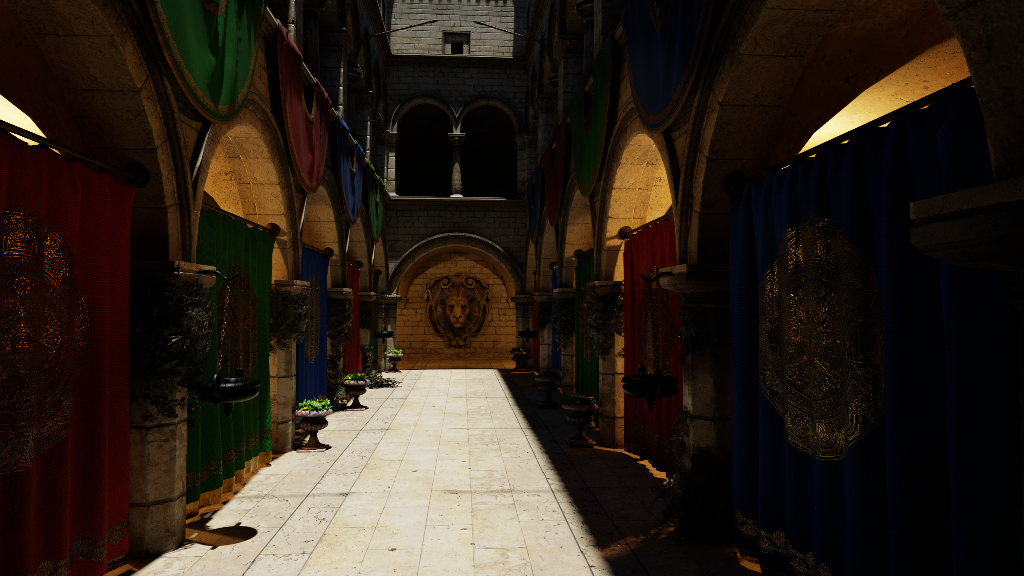
\includegraphics[width=0.85\textwidth]{figures/pt_ref.png}
\caption{Konvergirani referentni kadar iz ugra\dj enog path tracer-a, prema kome se u FLIP/PSNR/SSIM
mere sve real-time tehnike.}
\label{fig:pt-ref}
\end{figure}

\section{Uslovi i pretpostavke}
\label{sec:uslovi}

The implementation makes several deliberate approximations to stay within a real-time budget, each a
simplification of the full problem rather than a factor that distorts the relative measurements in
Chapter~\ref{ch:analiza}.

\begin{itemize}
  \item \textbf{Diffuse, single-bounce GI.} Global illumination computes one diffuse indirect bounce,
    while multi-bounce and glossy indirect are out of scope.
  \item \textbf{Half-resolution GI and AO.} GI and AO are traced at half resolution and bilaterally
    upsampled. Reflections are traced at full resolution.
  \item \textbf{Low sample counts with reconstruction.} Effects use one or two rays per pixel and
    depend on temporal accumulation, and on the spatial SVGF filter for GI and AO, for a usable
    image. The spatial filter is disabled for reflections (Section~\ref{sec:denoise-eval}).
  \item \textbf{Approximate soft shadows.} In the default path ray-traced shadows use one hard or two
    soft rays per light, traced inline and applied directly with no denoiser, so the penumbra is a
    two-sample approximation of an area light cleaned up only by the temporal resolve, not a
    converged soft shadow. The opt-in stochastic path does reconstruct its aggregate visibility
    through the shared denoiser, at the cost of resolving only one light per pixel per frame.
  \item \textbf{Inline ray queries only.} No ray-tracing pipeline, shader binding table, or
    recursion. All hit lighting is a single bounce evaluated in \texttt{ShadeSurfaceHit}.
  \item \textbf{Single-sample local-light NEE, GI only.} A GI secondary hit adds at most one of the
    scene's point and spot lights, importance-picked per hit rather than summed over all of them, so
    it remains a noisy, single-sample estimator of full next-event estimation rather than an exact
    sum. Reflections' hits are not extended with local lights at all (\texttt{render.rt.hit_lights}
    measured no quality gain there for twice the GI-side cost).
  \item \textbf{Full TLAS rebuild per dynamic frame.} The top-level structure is rebuilt, not refit,
    on any frame the scene changes, although a fully static scene skips the rebuild.
\end{itemize}

\chapter{Analiza}
\label{ch:analiza}

Every number reported in this chapter is produced by a measured run.

\section{Metodologija}
\label{sec:metodologija}

\paragraph{Hardver: cross-vendor postavka.} The central evaluation compares the identical pipeline on
two current-generation GPUs from different vendors: an AMD Radeon RX 9070 XT (RDNA4) and an NVIDIA
GeForce RTX 5070 (Blackwell), specified in Table~\ref{tab:gpus}. Both run the same engine binary, the
same SPIR-V shaders, the same render graph, and the same scene and settings; the only variable is the
selected physical device, which is the fairness basis: any difference in timing is due to the
hardware and its driver rather than to a different code path, and a quality divergence would point at
a non-determinism worth investigating rather than at a real difference. The one documented exception
to the identical-code-path claim is opacity micromap support.

\begin{table}[tbp]
\caption{GPU-ovi u cross-vendor pore\dj enju, prema zvani\v{c}nim specifikacijama proizvo\dj a\v{c}a
(AMD, NVIDIA) i verzijama drajvera sa test ma\v{s}ine.}
\label{tab:gpus}
\centering
\begin{tabularx}{\textwidth}{l >{\raggedright\arraybackslash}X >{\raggedright\arraybackslash}X}
\toprule
 & AMD RX 9070 XT & NVIDIA RTX 5070 \\
\midrule
Arhitektura            & RDNA4 (Navi 48) & Blackwell (GB205) \\
Compute jedinice / SM  & 64 CU, 4096 stream procesora & 48 SM, 6144 CUDA jezgara \\
RT akceleratori        & 64 (3. generacija) & 48 \\
Takt (boost)           & 2970 MHz & 2512 MHz \\
Memorija / propusnost  & 16 GB GDDR6, 640 GB/s & 12 GB GDDR7, 672 GB/s \\
TDP (TBP / TGP)        & 304 W & 250 W \\
Drajver / OS           & 32.0.31035.1003, Windows 11 Pro (build 26100) & 32.0.15.9186, Windows 11 Pro (build 26100) \\
\bottomrule
\end{tabularx}
\end{table}

\paragraph{Nesaglasje u podr\v{s}ci za OMM.} Sponza carries three MASK-mode (alpha-cutout) materials, which
trace through the opacity-micromap BLAS on a device exposing \texttt{VK\_EXT\_opacity\_micromap} and
through the any-hit alpha-test fallback otherwise (Section~\ref{sec:accel}). The RTX 5070 driver
exposes the extension and the 9070 XT driver does not, despite comparable hardware capability, so the
two vendors resolve masked geometry through genuinely different acceleration-structure code here. The
disparity only changes how a masked microtriangle is classified during traversal, not ray direction,
hit position or shading, so it cannot explain a quality-metric difference. It is a small,
one-directional, driver-dependent contributor to the per-effect GPU-ms gap wherever a ray hits cutout
geometry, and this evaluation does not isolate it further.

\paragraph{Scena i kontrole.} The test scene is Sponza, a standard interior with strong indirect
bounce, lit by five enabled lights: four point torches and one directional sun. Three spot lights and
two further point lights are authored but disabled, and the distinction matters because the default
shadow path costs one ray per light per pixel.

One property of the raster path bounds every technique that uses it: the engine allocates at most two
omni shadow maps (\texttt{MAX\_SHADOW\_POINTS}, six depth passes each), so two of the four enabled
point lights render unshadowed. Ray-traced shadows have no such cap, tracing one ray per light, so
every technique in Table~\ref{tab:quality} except \texttt{sve RT} sits on a weaker shadow baseline
than a renderer without that limit, which flatters the ray-traced side. The effect is bounded and
small: the shadow technique alone moves PSNR 0.65 dB of the 15.68 dB between raster and all effects,
and FLIP 0.024 of 0.349, so the lift in Section~\ref{sec:poredjenje} is dominated by global
illumination rather than by this cap.

Every measurement in this chapter renders at
$1915 \times 1064$, with the camera held static for every A/B comparison, since a moving camera
desynchronizes the frame sequence between two runs and fabricates differences that are timing
artifacts. The shader cache is cleared before any GPU metric is trusted, since a stale cache produces
nondeterministic results, and persisted console variables are ignored during a benchmark run, so a
leftover setting cannot silently change the configuration. Performance baselines are per-machine and
per-resolution, because absolute milliseconds are not comparable across GPUs or output sizes.

\paragraph{Merenje performansi.} GPU time comes from the per-pass timestamp scopes and the
\texttt{perf-bench} harness of Section~\ref{sec:alati}, averaged over a fixed frame budget once a
steady state has been detected rather than assumed: frame time takes about fifty frames to settle on
this scene, so a fixed short warmup would average part of the clock ramp into the result, by an
amount depending on how warm the machine already was and with nothing in the output to indicate it.
The benchmark sweeps a fixed
matrix of configurations, \texttt{rt-off} $\rightarrow$ \texttt{shadows} $\rightarrow$ \texttt{+ao}
$\rightarrow$ \texttt{+refl} $\rightarrow$ \texttt{+gi}, enabling one more effect at each step, so the
cost of an effect is the difference between adjacent configurations. A difference rather than an
isolated timing, because effects share fixed work (acceleration structure built once, G-buffer filled
once, tonemap run once): timing an effect alone would charge it for all of that, and the four figures
would then sum to considerably more than the frame costs.
The difference is taken on \emph{total} GPU time rather than on one pass scope, since
inline shadows are traced inside the Forward pass and have none of their own; the other three
effects do, and are reported as whole-frame deltas anyway for consistency. A
trailing \texttt{ssgi} configuration swaps ray-traced GI for the screen-space producer on top
of \texttt{+refl} and is diffed against \texttt{+refl}, since the two are alternatives rather than
cumulative. Timestamps are converted with each device's timestamp period, so
per-pass times are comparable across vendors, and both GPUs are reported side by side rather
than against a single-machine baseline, since the cross-vendor comparison is itself the
measurement.

\paragraph{Merenje kvaliteta.} Reconstruction quality is measured by \texttt{quality-bench} against
the converged path-traced reference of Section~\ref{sec:pathtracer}. Each real-time technique's
tonemapped present is scored against it by \textbf{FLIP} (perceptual), \textbf{PSNR} and
\textbf{SSIM}. FLIP is primary because it models what a human observer notices rather than raw
per-pixel error; PSNR structurally favours a blurrier image and SSIM compares local structure rather
than absolute values, so all three are reported and no single metric's bias decides a conclusion.
Scores are averaged over three fixed orientations from one interior position (down the nave, tilted
to the floor, tilted to the upper gallery), chosen to stress ambient occlusion, global illumination
and reflections differently, so a single framing cannot bias the result. Each capture is bilinearly
resampled to a canonical $1024 \times 576$ first, so a window-size difference between runs cannot
silently change a score. Quality figures elsewhere in this chapter are
the RX 9070 XT's; Section~\ref{sec:cross-vendor-quality} captures the whole matrix on the RTX 5070 as
well.

\section{Cena po efektu (GPU ms)}
\label{sec:cena}

\begin{table}[tbp]
\caption{Cena po efektu (GPU ms) na cross-vendor paru RX 9070 XT / RTX 5070, pri rezoluciji
$\perfWidth \times \perfHeight$ i fiksiranoj pozi kamere, prosek preko \perfFrames{} frejmova.
\texttt{rt-off} je ukupno GPU vreme bez RT efekata; svaki naredni red je dodatak (delta) tog efekta u
odnosu na prethodnu konfiguraciju. Red \texttt{ssgi} je alternativa za \texttt{+gi} (screen-space GI
umesto RT GI) i pore\dj en je sa \texttt{+refl}, ne kumulativno sa \texttt{+gi}. Sve vrednosti se
generi\v{s}u iz committovanih baseline-a skriptom \texttt{tools/gen\_perf\_tables.py}.}
\label{tab:cena}
\centering
\begin{tabular}{llrr}
\toprule
Configuration & Effect & ms (9070 XT) & ms (5070) \\
\midrule
\texttt{rt-off}   & baseline (total) & 2.274 & 1.347 \\
\texttt{+shadows} & shadows & 2.272 & 1.294 \\
\texttt{+ao} & ambient occlusion & 0.817 & 0.728 \\
\texttt{+refl} & reflections & 1.756 & 1.291 \\
\texttt{+gi} & global illumination (RT) & 1.705 & 1.309 \\
\midrule
\texttt{+gi} & \textbf{total, all effects} & \textbf{8.824} & \textbf{5.970} \\
\midrule
\texttt{ssgi} & screen-space GI (alternative to +gi) & 0.739 & 0.667 \\
\bottomrule
\end{tabular}

\end{table}

In Table~\ref{tab:cena} the per-effect rows are differences, although the total is the measured
whole-frame time of the \texttt{+gi} configuration rather than their sum, so rounding cannot
accumulate. Table~\ref{tab:pass-cost} breaks that same frame down by pass.

\begin{table}[tbp]
\caption{Najskuplji prolazi u \texttt{+gi} konfiguraciji (GPU ms, prosek preko \perfFrames{}
frejmova). \texttt{Forward} sadr\v{z}i i inline RT senke, pa nema zaseban scope. GI i AO filtriraju u
polovi\v{c}noj rezoluciji. Prolazi za denoise-ovanje refleksija ne pojavljuju se u tabeli jer se vi\v{s}e
ne izvr\v{s}avaju: \texttt{render.reflections.denoise.iterations} je sada 0
(odeljak~\ref{sec:denoise-eval}).}
\label{tab:pass-cost}
\centering
\begin{tabular}{lrr}
\toprule
Pass & ms (9070 XT) & ms (5070) \\
\midrule
\texttt{Forward} (includes inline shadows) & 4.444 & 2.396 \\
\texttt{Reflection} & 1.495 & 1.136 \\
\texttt{GI} & 1.076 & 0.725 \\
\texttt{GIDenoise*} & 0.329 & 0.317 \\
\texttt{AODenoise*} & 0.330 & 0.309 \\
\texttt{AO} & 0.170 & 0.199 \\
\texttt{DepthNormal} & 0.142 & 0.231 \\
\texttt{TemporalResolve} (TAA) & 0.177 & 0.090 \\
\bottomrule
\end{tabular}

\end{table}


\begin{figure}[tbp]
\centering
\begin{tikzpicture}
\begin{axis}[width=0.88\textwidth, height=6.4cm,
  xlabel={konfiguracija}, ylabel={ukupno GPU (ms)},
  xtick={0,1,2,3,4},
  xticklabels={\texttt{rt-off},\texttt{shadows},\texttt{+ao},\texttt{+refl},\texttt{+gi}},
  ymin=0, grid=major, grid style={black!12},
  tick label style={font=\small}, label style={font=\small},
  legend style={at={(0.02,0.98)}, anchor=north west, font=\small, draw=black!30}]
\addplot[thick, mark=*] table[col sep=tab, x=i, y=amd] {data/ladder.dat};
\addplot[thick, mark=square*, dashed] table[col sep=tab, x=i, y=nv] {data/ladder.dat};
\legend{RX 9070 XT, RTX 5070}
\end{axis}
\end{tikzpicture}
\caption[Kumulativno GPU vreme kroz lestvicu konfiguracija]{Ukupno GPU vreme kroz lestvicu, gde svaka
sledeca konfiguracija uklju\v{c}uje jo\v{s} jedan efekat. Nagib segmenta je cena tog efekta. Obe
kartice rastu monotono, ali AMD kre\'ce vi\v{s}e i raste br\v{z}e, pa se razmak \v{s}iri sa 0.93 ms na
\texttt{rt-off} do 2.85 ms na \texttt{+gi}.}
\label{fig:ladder}
\end{figure}

\begin{figure}[tbp]
\centering
\begin{tikzpicture}
\begin{axis}[xbar, bar width=5pt, width=0.62\textwidth, height=9.5cm,
  xlabel={odnos AMD / NVIDIA (GPU ms)},
  xmin=0, xmax=2.2, y dir=reverse,
  ytick={0,...,15}, yticklabels from table={data/passcost-vendor.dat}{pass},
  yticklabel style={font=\footnotesize}, tick label style={font=\small},
  label style={font=\small}, grid=major, grid style={black!12},
  nodes near coords, nodes near coords style={font=\tiny, /pgf/number format/fixed,
    /pgf/number format/precision=2}]
\addplot[fill=black!18, draw=black!55] table[col sep=tab, x=ratio, y expr=\coordindex]
  {data/passcost-vendor.dat};
\draw[dashed, black!60] (axis cs:1,-1) -- (axis cs:1,16);
\end{axis}
\end{tikzpicture}
\caption[Odnos cene po prolazu izme\dj u proizvo\dj a\v{c}a]{Cena svakog prolaza na AMD-u podeljena
cenom istog prolaza na NVIDIA-i, u \texttt{+gi} konfiguraciji. Isprekidana linija je paritet. Desno od
nje NVIDIA je br\v{z}a, levo AMD. Raspon od 0.62 do 1.96 pokazuje da razlika nije jedan globalni
faktor takta: \texttt{Forward} (koji nosi inline senke) i \texttt{TemporalResolve} idu jako u korist
NVIDIA-e, dok tre\'ca a-trous iteracija i \texttt{DepthNormal} idu u korist AMD-a.}
\label{fig:vendor-ratio}
\end{figure}

The two cards do not agree on which effect is most expensive. On the RX 9070 XT shadows dominate at
\perfEffShadowsAMD{} ms, well clear of reflections and global illumination. On the RTX 5070 those
same three fall within \perfNVSpread{} ms of each other, inside the run-to-run spread, so on that
card they are indistinguishable in cost. Ambient occlusion is cheapest on both. Together the four add
\perfFourEffectsAMD{} ms (9070 XT) and \perfFourEffectsNV{} ms (5070) over their respective
baselines, for measured real-time totals of \perfTotalAMD{} ms (\perfBaseAMD{} ms baseline) and
\perfTotalNV{} ms (\perfBaseNV{} ms baseline).

The half-resolution trace plus denoise is what keeps GI and AO cheap despite their hemispheric
gather. On both cards the screen-space GI producer is cheaper than ray-traced GI at the same rung
(9070 XT 0.739 against 1.705 ms; RTX 5070 0.667 against 1.309 ms), the expected
screen-space-versus-ray-traced cost tradeoff, whose quality side is Section~\ref{sec:poredjenje}.

Reflections are no longer the most expensive effect, and the reason is a deliberate default change
rather than an optimisation: the reflection à-trous filter measured net-negative and now runs zero
iterations (Section~\ref{sec:denoise-eval}), removing a full-resolution three-pass chain worth roughly
1.1 ms. They remain the only effect tracing at full resolution, so their trace alone (1.495 ms on the
9070 XT) costs more than the half-resolution GI trace. Ambient occlusion is cheapest despite casting
more rays per pixel, because those rays are short (bounded by \texttt{render.ao.radius}) and
terminate on the first hit, while a reflection ray can traverse the whole scene and then shade what
it finds.

Shadows have no scope of their own, so their cost has to be read across configurations. Between
\texttt{rt-off} and \texttt{shadows} on the 9070 XT the Forward pass grows by 3.482 ms while the
raster shadow-map passes disappear entirely, returning 1.056 ms (\texttt{Shadow} 0.107 and
\texttt{PointShadows} 0.949). Those two terms give 2.426 ms against a measured whole-frame delta of
2.272 ms; the remaining 0.154 ms is every other pass shrinking slightly at once, the signature of a
clock shift rather than of real savings, consistent with \texttt{rt-off} being the noise-dominated
configuration on this adapter (8.3\% run-to-run spread against under 1\% for the others). The
whole-frame difference is the number to quote, since the per-pass terms do not close.

\begin{figure}[tbp]
\centering
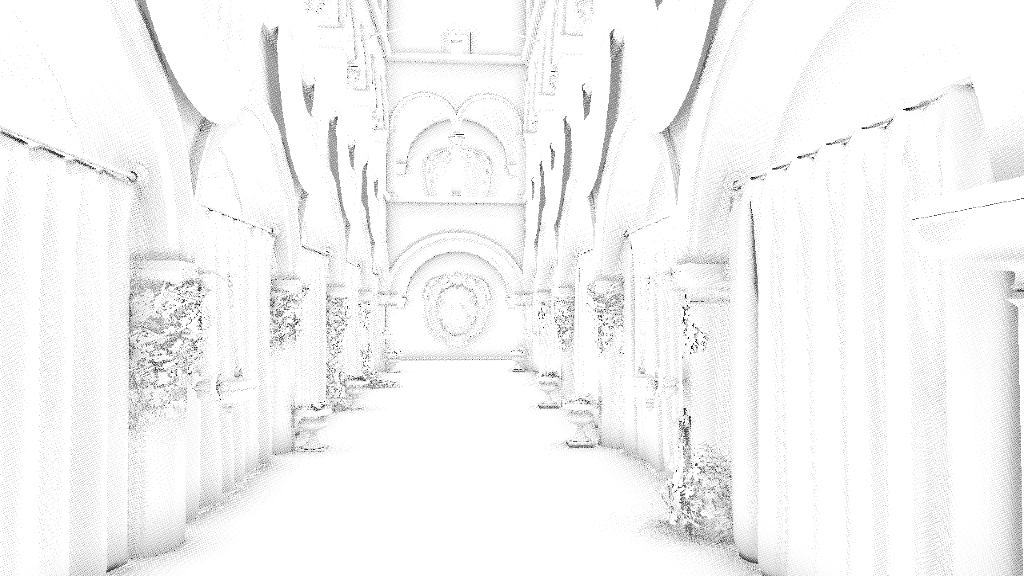
\includegraphics[width=0.48\textwidth]{figures/dbg_ao.png}\hfill%
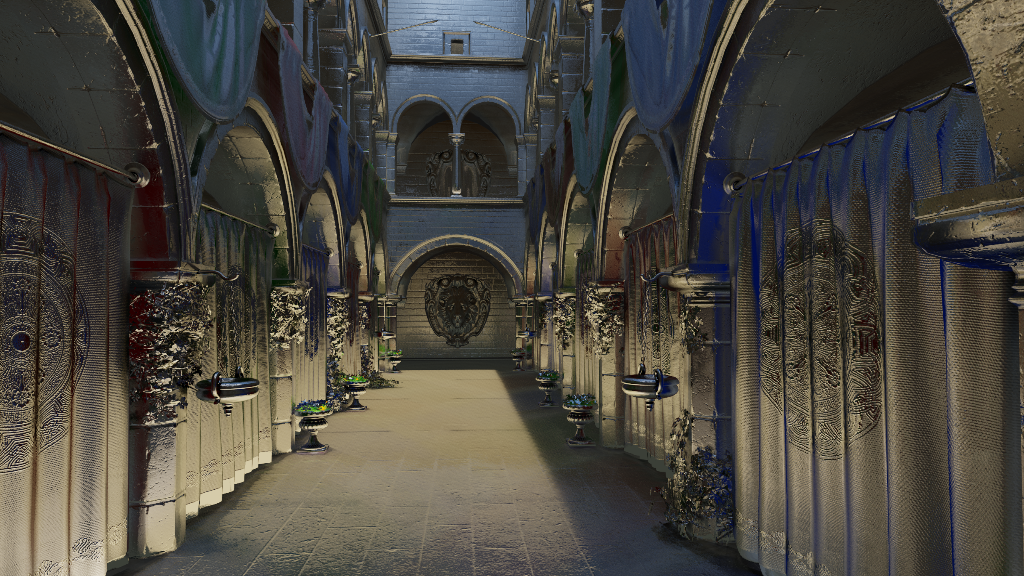
\includegraphics[width=0.48\textwidth]{figures/dbg_refl.png}

\vspace{5pt}

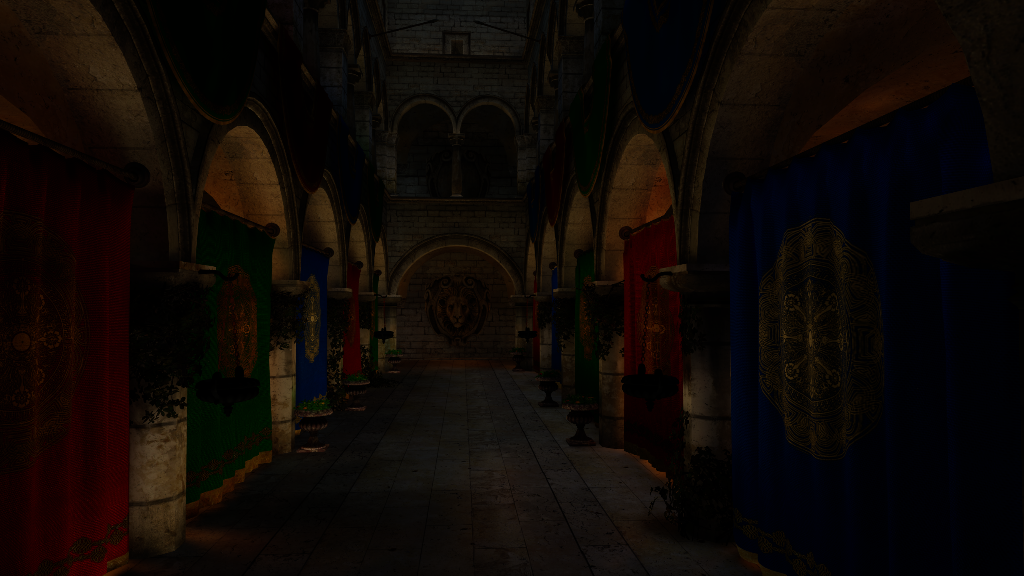
\includegraphics[width=0.48\textwidth]{figures/dbg_gi.png}\hfill%
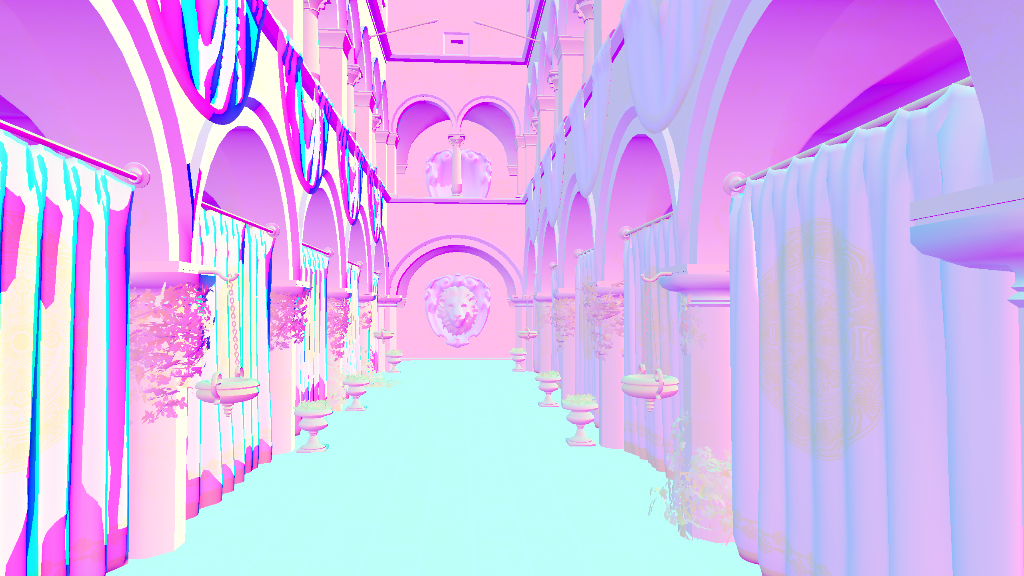
\includegraphics[width=0.48\textwidth]{figures/dbg_normals.png}
\caption{Pojedina\v{c}ni signali izolovani preko \texttt{render.debugview}, ista scena i kamera:
ambijentalna okluzija (gore levo), reflektovana radijansa (gore desno), indirektni GI \v{c}lan
(dole levo) i normale iz G-buffer-a (dole desno). Prikazani su sirovi me\dj urezultati pre
kombinovanja u forward prolazu, a ne gotova slika.}
\label{fig:effect-gallery}
\end{figure}

Toggling shadows, ambient occlusion or reflections individually moves the final image by a mean of
only 2.1 to 2.5 levels out of 255 at this viewpoint, while global illumination moves it by 23.9. The
ambient-occlusion buffer is close to white over most of the frame because Sponza's atrium is open, so
occlusion is confined to the arcade vaults and the column bases; the raw GI term is dim in absolute
terms yet carries the colour bleeding (the red and green drapes tinting the stone beside them) that a
constant ambient cannot reproduce.

\section{Dve strategije za senke: inline naspram stohasti\v{c}ke}
\label{sec:analiza-shadow-strategy}

The two shadow strategies of Section~\ref{sec:senke} have differently shaped cost curves: the default
inline path traces one ray per light per pixel inside the forward shader, while the stochastic path
picks one light per pixel by resampled importance sampling and reconstructs the result with the
shared denoiser.

\begin{table}[tbp]
\caption{Dve strategije za senke na istoj sceni sa pet upaljenih svetala (GPU ms, dodatak u odnosu na
\texttt{rt-off}).}
\label{tab:shadow-strategy}
\centering
\begin{tabular}{lrr}
\toprule
Strategy & ms (9070 XT) & ms (5070) \\
\midrule
inline, per light (default) & 2.272 & 1.294 \\
stochastic, RIS + denoiser & 1.723 & 3.362 \\
\bottomrule
\end{tabular}

\end{table}

The two cards disagree about which strategy is cheaper. On the RX 9070 XT the stochastic path wins,
1.723 ms against 2.272 ms. On the RTX 5070 it loses badly, 3.362 ms against 1.294 ms, a factor of
2.6.

The stochastic path replaces per-light rays with one importance-sampled ray plus a reconstruction
chain, trading ray count for filter cost, which pays exactly when rays are expensive relative to
filtering. On the 5070 they are not: dedicated traversal hardware makes the twenty coherent inline rays of a five-light scene
cheap enough that paying a temporal pass, three à-trous iterations, and an upsample to avoid them is a
net loss. On the 9070 XT, where traversal is driven by shader instructions and competes with shading
for the same execution resources (Section~\ref{sec:accel-pregled}), the same trade pays.

The choice of shadow technique is therefore a property of the target architecture: a renderer that
hard-codes either strategy is wrong on one of these two cards, and a single-vendor evaluation cannot
see that.

Two caveats bound the claim. The stochastic path's cost is nearly independent of light count while the
inline path's grows with it, so five lights is one point on two curves that must cross somewhere; this
scene cannot show where. And the stochastic producer is experimental and off by default, with known
artifacts under camera motion where two point lights overlap, so these are the numbers of a prototype
rather than of a shipping technique.

\section{Broj zrakova naspram kvaliteta i brzine}
\label{sec:raycount}

The GI ray count per pixel is swept through the full pipeline (denoiser and temporal resolve enabled,
settled over 90 frames, RX 9070 XT), scoring reconstruction quality against the path-traced reference
and GPU time against the ray count.

\begin{table}[htb]
\centering
\caption{GI kvalitet i GPU cena u funkciji broja zraka po pikselu (denoiser i temporalni resolve
uklju\v{c}eni, RX 9070 XT).}
\label{tab:raycount}
\begin{tabular}{@{}rrrrr@{}}
\toprule
Rays/pixel & PSNR (dB) & SSIM & FLIP & GPU total (ms) \\
\midrule
1 & 24.52 & 0.7356 & 0.1486 & 3.51 \\
2 & 24.65 & 0.7395 & 0.1449 & 3.85 \\
4 & 24.67 & 0.7407 & 0.1458 & 4.28 \\
8 & 24.73 & 0.7432 & 0.1433 & 6.43 \\
\bottomrule
\end{tabular}

\end{table}

The knee sits at 1 ray per pixel. Going from 1 to 8 rays costs \rcGpuPct\% more GPU time
(\rcGpuLow{} to \rcGpuHigh{} ms) for a \rcPsnrGain{} dB PSNR gain and a FLIP improvement from
\rcFlipLow{} to \rcFlipHigh{}, both within run-to-run noise on
this metric. The denoiser and temporal accumulation already recover most of the achievable quality
from a single ray, so additional samples per pixel are not where this engine's ray budget should go.
This is consistent with the SVGF design goal (spatiotemporal
filtering to make 1 sample per pixel viable) rather than a property specific to this
implementation. Figure~\ref{fig:spp-sweep} shows the raw noise this filtering masks, captured with the
GI spatial denoiser, the GI temporal accumulation and TAA disabled, at a fixed 30-frame cap.
Disabling TAA is what makes the figure honest: TAA is itself a temporal
accumulator, so with it enabled the capture settles into the same smoothness as the denoised image and
the ray count appears to make no difference at all.

Quantifying that needs a measure of per-pixel roughness. Define the \emph{high-frequency energy} of an
image as the mean absolute difference between vertically adjacent pixels of its grayscale channel,
$\frac{1}{(H-1)W}\sum_{y,x} |g_{y+1,x} - g_{y,x}|$, computed on the 8-bit tonemapped capture; noise
raises it, blur lowers it, and it can be recomputed from the committed figures. With TAA enabled, one
ray per pixel and the fully denoised image both score 5.9, which is the measurement saying the figure
would show nothing. With TAA disabled the ray count separates cleanly: 10.8, 9.1, 8.1, and 7.3 for
one, two, four, and eight rays per pixel, monotonically approaching the reference as the sample count
rises.

\begin{figure}[tbp]
\centering
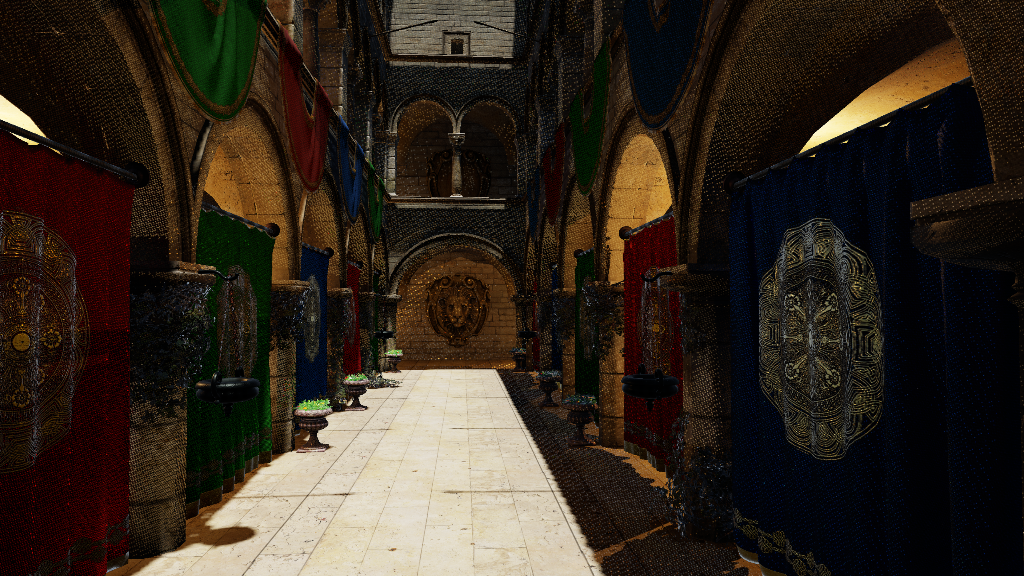
\includegraphics[width=0.48\textwidth]{figures/spp_sweep_1.png}\hfill%
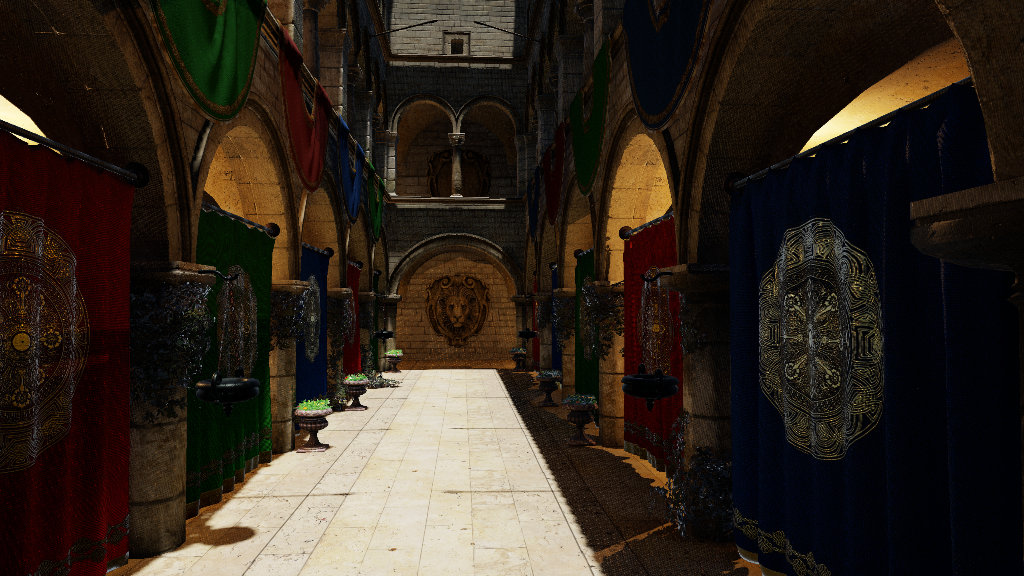
\includegraphics[width=0.48\textwidth]{figures/spp_sweep_8.png}
\caption{Uticaj broja zraka po pikselu na \v{s}um pre denoise-a, pre temporalnog resolve-a i bez TAA
(GI; levo 1 zrak, desno 8 zrakova po pikselu): vi\v{s}e zraka konvergira ka referenci, uz
proporcionalno ve\'cu cenu (Tabela~\ref{tab:raycount}).}
\label{fig:spp-sweep}
\end{figure}

\section{Polovi\v{c}na naspram pune rezolucije}
\label{sec:halfres}

Tracing the two hemispheric gather effects at half resolution is the single largest cost decision in
the renderer (Section~\ref{sec:rendergraph}). Setting \texttt{render.gi.scale} and \texttt{render.ao.scale} to 1.0 turns it off, changing nothing else, so
the two configurations differ in exactly one variable.

\begin{table}[tbp]
\caption{Polovi\v{c}na naspram pune rezolucije za GI i AO trasiranje (RX 9070 XT). Vreme je ukupno GPU
vreme \texttt{+gi} konfiguracije; kvalitet je meren iz atrijumskog pogleda naspram konvergirane
path-traced reference.}
\label{tab:halfres}
\centering
\begin{tabular}{lrrr}
\toprule
 & half (0.5) & full (1.0) & difference \\
\midrule
Total GPU (ms) & 8.67 & 13.34 & $+54\%$ \\
\texttt{GI} pass (ms) & 1.07 & 4.12 & $\times 3.8$ \\
\texttt{AO} pass (ms) & 0.17 & 0.63 & $\times 3.8$ \\
\midrule
PSNR (dB) & 29.58 & 29.58 & $+0.00$ \\
SSIM & 0.8702 & 0.8710 & $+0.0008$ \\
FLIP & 0.1027 & 0.1025 & $-0.0002$ \\
\bottomrule
\end{tabular}

\end{table}

Full-resolution tracing costs \hrDeltaMs{} ms more per frame, a \hrDeltaPct\% increase on a
\hrHalfTotal{} ms budget, and returns \hrPsnrGain{} dB of PSNR: the two configurations are identical
to the second decimal. SSIM and FLIP move by 0.0008 and 0.0002, both far inside the run-to-run
spread. The reading is not \rqt{full resolution is slightly better} but \rqt{the measurement cannot
distinguish them at all}.

The reason is that the denoiser is the binding constraint, not the sample grid. Both configurations
feed the same à-trous filter, whose edge-stopping kernel already blurs over a neighbourhood wider than
the factor of two separating them; the extra samples are averaged away by the very filter that makes
the half-resolution result usable. The half-resolution plus bilateral-upsample pattern is therefore
close to free rather than a quality compromise accepted for speed.

Figure~\ref{fig:halfres-buffer} shows the raw GI irradiance under both settings, taken through the
debug view that bypasses the upsample, denoiser and composite. The half-resolution buffer carries
44\% more high-frequency energy by the roughness proxy of Section~\ref{sec:raycount} (41.68
against 28.91). That proxy is reproducible where the per-pixel difference is not: a second
full-resolution capture with identical settings scores 28.85, within 0.2\%, while differing from the
first by 18.3 grey levels per pixel simply because the two traces drew different random samples. So
the per-pixel gap of 35.4 between the half- and full-resolution buffers is only about twice the
run-to-run floor and carries little information, whereas the roughness gap is far outside it. Four
times the rays do produce a measurably cleaner buffer; what Table~\ref{tab:halfres} shows is that
nothing downstream of the filter preserves it.

\begin{figure}[tbp]
\centering
\begin{minipage}{0.48\textwidth}\centering
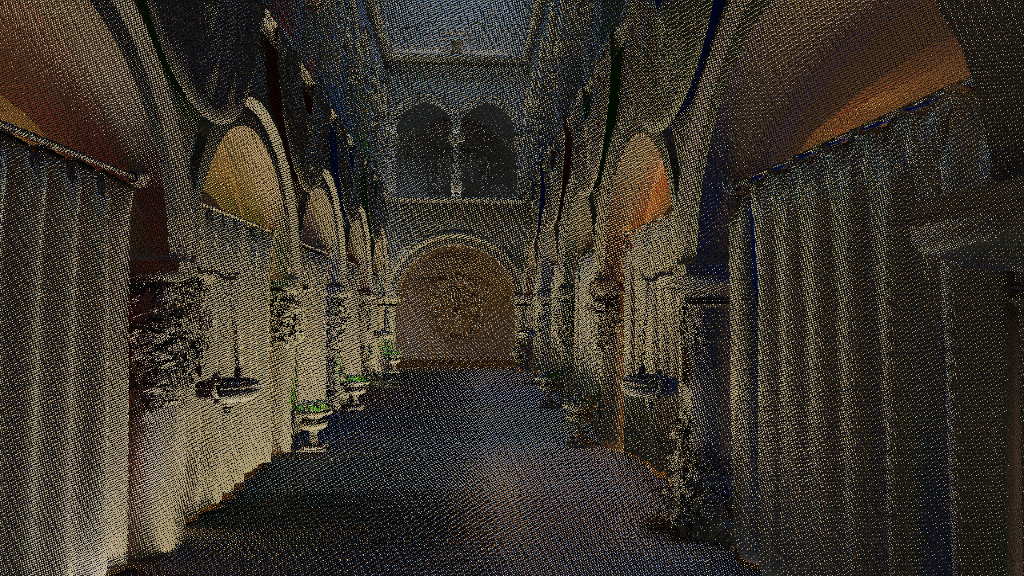
\includegraphics[width=\linewidth]{figures/gi_halfres.png}\\{\small polovi\v{c}na (0.5)}
\end{minipage}\hfill
\begin{minipage}{0.48\textwidth}\centering
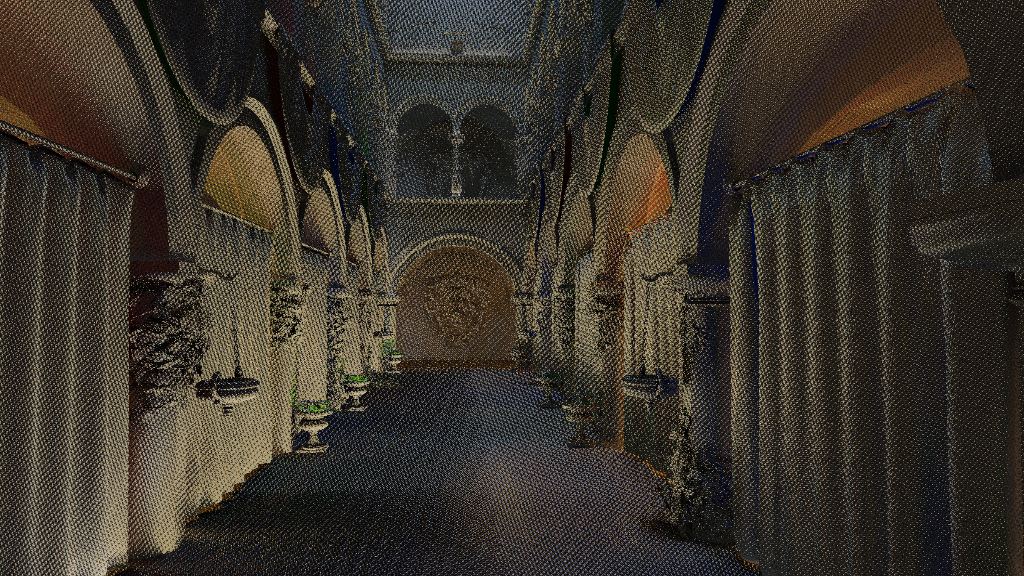
\includegraphics[width=\linewidth]{figures/gi_fullres.png}\\{\small puna (1.0)}
\end{minipage}
\caption[Sirov GI bafer: polovi\v{c}na naspram pune rezolucije]{Sirov GI bafer pre upsample-a i denoiser-a, pri \texttt{render.gi.scale} 0.5 i 1.0
(\texttt{render.debugview} 6). Puna rezolucija daje finiju zrnastost: 28.91 naspram 41.68 po meri
visokofrekventne energije. U finalnoj slici se ta razlika ne meri (Tabela~\ref{tab:halfres}).}
\label{fig:halfres-buffer}
\end{figure}

Two caveats bound that claim. The quality figures come from one viewpoint rather than the three-view
average used elsewhere, and the conclusion is specific to diffuse gather signals: as
Section~\ref{sec:rendergraph} argues, the same treatment applied to shadows or reflections would
destroy exactly the high-frequency detail those effects exist to produce, which is why neither is
traced at half resolution in the first place.

\section{Evaluacija denoiser-a (SVGF)}
\label{sec:denoise-eval}

The SVGF spatial denoiser's own contribution is isolated by holding temporal accumulation constant
(enabled in both states, settled over 90 frames) and scoring the noisy input against the denoised
result against the path-traced reference, at a fixed 2 rays per pixel, RX 9070 XT.

\begin{table}[htb]
\centering
\caption{Doprinos SVGF denoiser-a naspram path-traced reference (2 zraka/piksel, temporalni resolve
uklju\v{c}en u oba slu\v{c}aja).}
\label{tab:denoise-eval}
\begin{tabular}{@{}lrrr@{}}
\toprule
Denoiser & PSNR (dB) & SSIM & FLIP \\
\midrule
off & 24.67 & 0.7409 & 0.1446 \\
on & 24.65 & 0.7397 & 0.1449 \\
\bottomrule
\end{tabular}

\end{table}

With temporal accumulation already active, the spatial SVGF pass changes the static-frame metrics
(PSNR, SSIM, FLIP) by less than measurement noise: the temporal history is doing essentially all of
the visible convergence at this settled frame, and the filter's own contribution shows up in temporal
stability instead. A frame-to-frame RMS delta on the same static view (frame $N$ against $N{+}1$ at
steady state, a flicker proxy under a static camera, not motion) drops only from \flickerOff{} with
the denoiser off to \flickerOn{} with it on, a \flickerPct\% reduction. That figure is sensitive to
one protocol detail: unless temporal history is cleared before sampling, the unfiltered case is
credited with noise that accumulated while assets were still streaming, which inflates the apparent
reduction to near 40\%, so figures captured with and without that clear are not comparable. The
denoiser's GPU cost is read from its own timestamp scopes rather than from a whole-frame A/B: the
three \texttt{GIDenoise} à-trous iterations total \perfDenoiseAMD{} ms on the 9070 XT and
\perfDenoiseNV{} ms on the 5070 (Table~\ref{tab:pass-cost}), against a full-frame budget near nine
milliseconds, and they are cheap partly because they run at half resolution. Toggling the denoiser
and diffing whole-frame totals gives about 0.07 ms, which should not be quoted: it is smaller than
the run-to-run spread of the identical configuration, so it measures noise rather than the filter.

Debug views 6 and 7 isolate the filter from everything else in the image, showing the half-resolution
GI irradiance buffer as the trace leaves it and after temporal accumulation plus the à-trous, before
either is upsampled or composited (Figure~\ref{fig:gi-denoise-ab}). The high-frequency energy defined
in Section~\ref{sec:raycount} falls from \hfGiRaw{} to \hfGiDenoised{} between the two, some 96\% of
it, while the mean level rises because the filter fills in the pixels where every ray happened to
miss.

So the filter transforms the intermediate buffer almost completely, and yet the finished image is
unchanged to within measurement noise. The pipeline downstream absorbs the work: the buffer is
upsampled from half resolution, multiplied by surface albedo, added to direct lighting that dominates
it, then run through a temporal resolve that is itself a strong low-pass in time. At two rays per pixel with
temporal accumulation already active, the spatial à-trous is close to redundant for global
illumination and worse than redundant for reflections, which is why it is kept at three iterations
for the former and disabled for the latter rather than applied uniformly, and it argues for spending
a reconstruction budget on the temporal side before the spatial one.

\paragraph{Isti filtar na refleksijama je \v{s}tetan.} The same à-trous runs on the reflection signal
and there it measured net-negative, which is why it is now disabled by default: turning it off
improved every spatial metric at once, FLIP 0.1742 against 0.1746, PSNR 21.75 against 21.70, SSIM
0.6473 against 0.6419. That all three move the same way is what separates this from metric gaming,
since the signature of merely deleting blur is FLIP and PSNR improving while SSIM drops. The
structural reason is that the filter is guided by the receiving surface's normal and depth, correct
for a diffuse gather although wrong for reflections: reflected radiance is view-dependent, so on a
flat reflective surface those guides are constant and the kernel opens wide exactly where reflected
detail lives. The chain ran at full resolution with no upsample after it, so removing it is most of
the 1.1 ms by which reflections became cheaper in
Table~\ref{tab:cena}. A roughness-driven kernel remains the structurally right fix, although it now
has to beat filtering off rather than beat three iterations.

\paragraph{Cena filtra nije ista na oba proizvo\dj a\v{c}a.} Rolling the à-trous outer loop, done to
cut the shader's register pressure (Section~\ref{sec:occupancy}), paid asymmetrically: on the RTX
5070 every stride got faster, while on the RX 9070 XT it was close to a wash on the half-resolution
GI and AO chains (first iteration slower, last one faster) and paid only on the full-resolution ones.
The per-pass table shows the residue: the AMD denoise chain is front-loaded (\texttt{GIDenoise0}
0.133 ms falling to 0.089 ms at \texttt{GIDenoise2}) while the NVIDIA one inverts (0.094 ms rising to
0.127 ms). The stride-1 iteration is the one where adjacent taps are cache-friendly enough that
batching beats occupancy, and that tradeoff lands differently on the two memory hierarchies. A shader
optimisation justified by a register count is therefore not automatically a win, and has to be
measured per vendor like everything else in this chapter.

\begin{figure}[tbp]
\centering
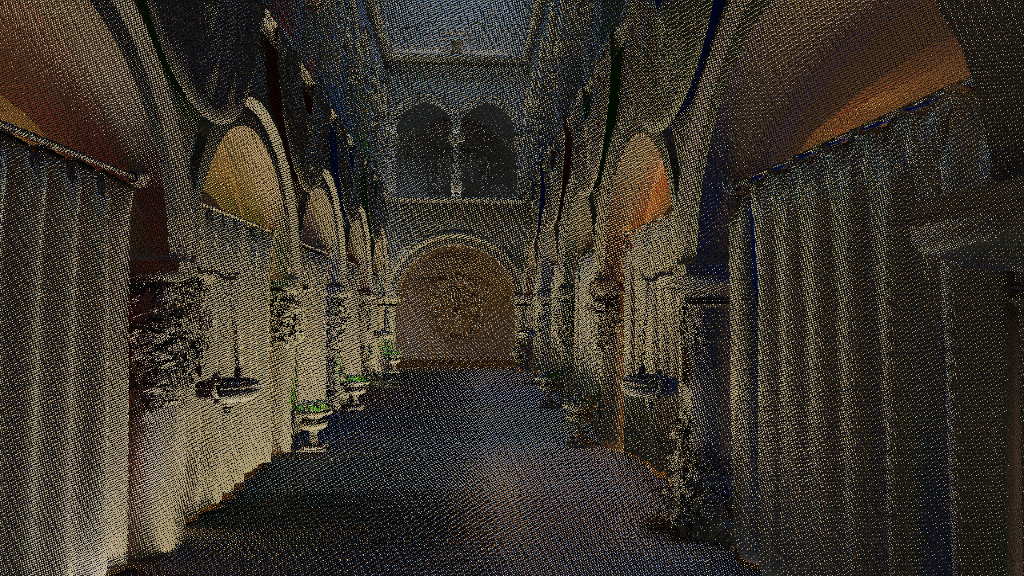
\includegraphics[width=0.48\textwidth]{figures/dbg_gi_raw.png}\hfill%
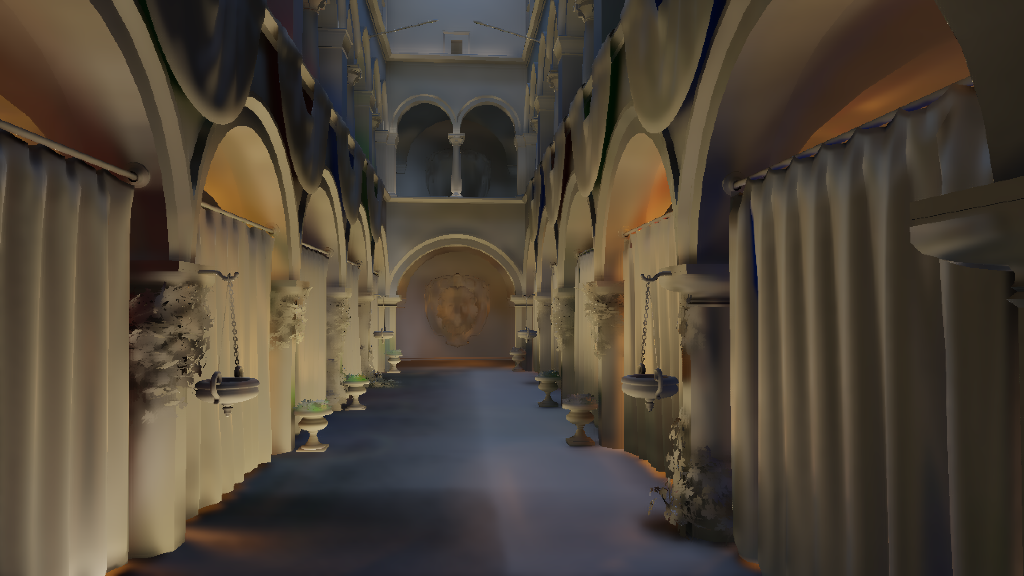
\includegraphics[width=0.48\textwidth]{figures/dbg_gi_denoised.png}
\caption{Polovi\v{c}na GI zra\v{c}nost pre (levo) i posle (desno) temporalne akumulacije i a-trous
filtra, pre upsample-a i kompozicije (\texttt{render.debugview} 6 i 7). Levo se vidi zrnasti
jednozra\v{c}ni signal, desno isti bafer nakon rekonstrukcije.}
\label{fig:gi-denoise-ab}
\end{figure}

\begin{figure}[tbp]
\centering
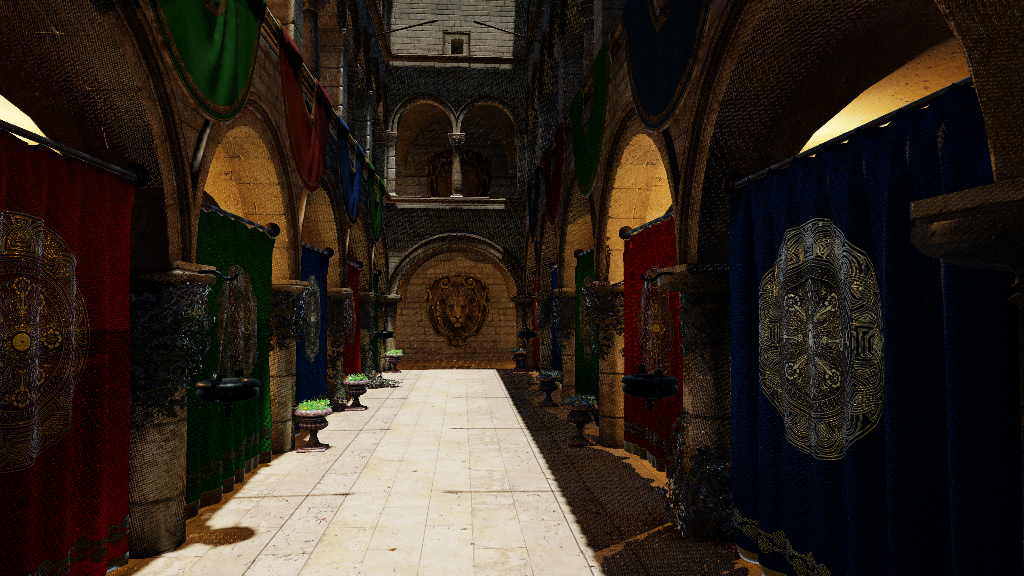
\includegraphics[width=0.62\textwidth]{figures/denoise_compare_noisy.png}

\vspace{5pt}

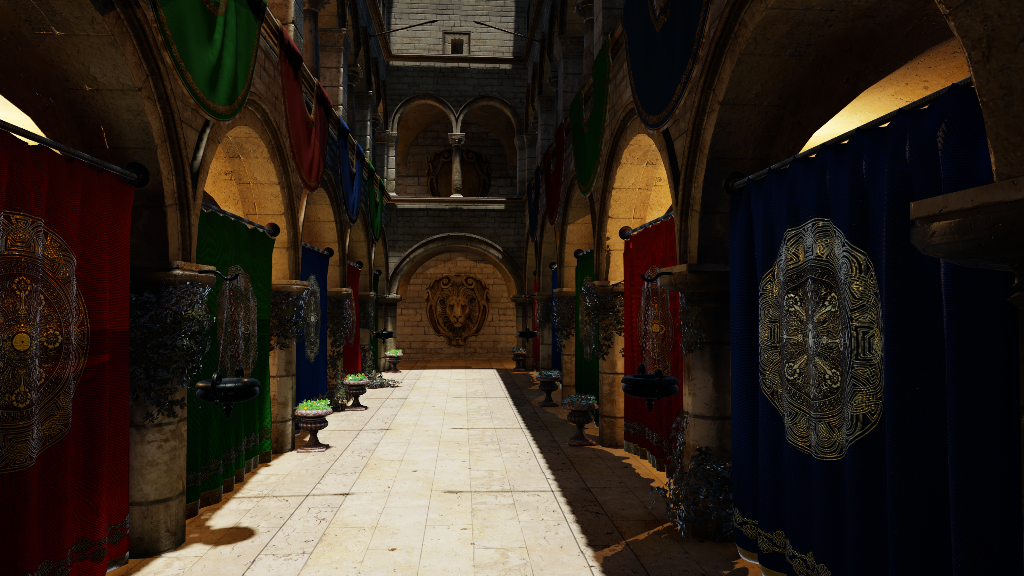
\includegraphics[width=0.62\textwidth]{figures/denoise_compare_denoised.png}

\vspace{5pt}

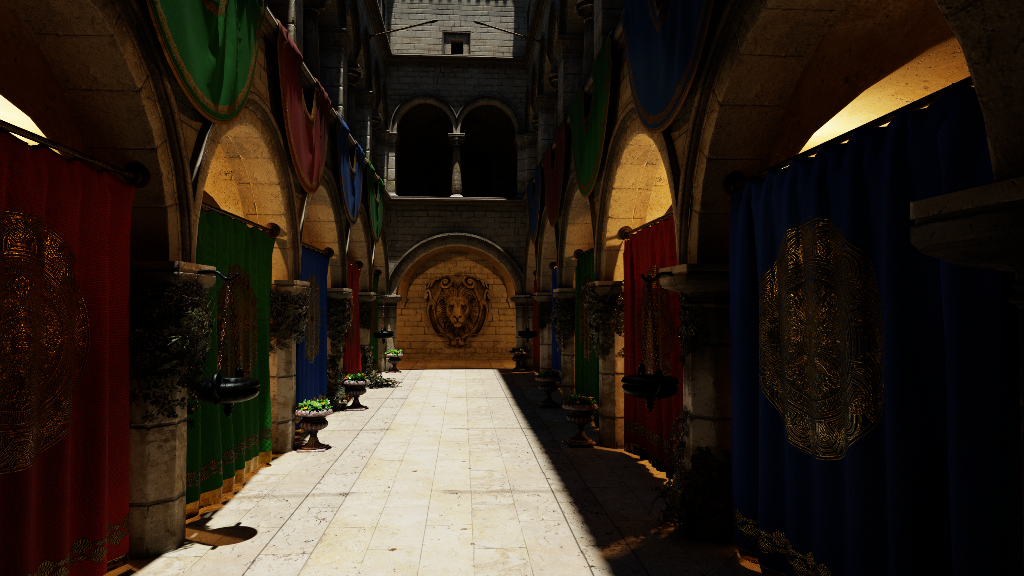
\includegraphics[width=0.62\textwidth]{figures/denoise_compare_reference.png}
\caption{Rekonstrukcija na 2 zraka po pikselu: sirov signal bez denoiser-a, temporalnog resolve-a i
TAA (gore), pun real-time rezultat sa sve tri komponente uklju\v{c}ene (sredina), i path-traced
referenca (dole). Razlika gore-sredina je doprinos cele rekonstrukcije; doprinos samog denoiser-a
izolovan je metrikama u tekstu, gde se vidi pre svega u temporalnoj stabilnosti.}
\label{fig:denoise-compare}
\end{figure}

\section{Pore\dj enje sa postoje\'cim re\v{s}enjima}
\label{sec:poredjenje}

The engine implements raster screen-space baselines for ambient occlusion and reflections (SSAO, SSR;
Section~\ref{sec:efekti}), so the comparison against the solutions surveyed in
Chapter~\ref{ch:pregled} is a same-scene, same-camera A/B, exposing the cases the screen-space method
structurally cannot handle: off-screen occluders and reflectors, and disocclusion
(Figure~\ref{fig:rt-vs-ss}). The positioning against production systems (Lumen, RTXGI, ReSTIR) is
qualitative: the contribution is an integrated, measured, openly licensed ray-query implementation,
not a system that beats a production global-illumination solution.

\begin{table}[tbp]
\caption{Kvalitet svake tehnike u odnosu na path-traced referencu (prosek preko tri pogleda: atrium,
floor, gallery; RX 9070 XT). Manji FLIP i ve\'ci PSNR/SSIM su bolji.}
\label{tab:quality}
\centering
\begin{tabular}{lrrr}
\toprule
Tehnika & FLIP $\downarrow$ & PSNR (dB) $\uparrow$ & SSIM $\uparrow$ \\
\midrule
raster (bez efekata) & 0.435 & 15.17 & 0.383 \\
SSAO                 & 0.418 & 15.61 & 0.398 \\
RT AO                & 0.414 & 15.71 & 0.400 \\
SSR                  & 0.429 & 15.31 & 0.395 \\
RT refleksije        & 0.422 & 15.44 & 0.404 \\
SSGI                 & 0.341 & 17.56 & 0.457 \\
RT GI                & 0.141 & 25.21 & 0.720 \\
sve RT (all-RT)      & \textbf{0.086} & \textbf{30.85} & \textbf{0.872} \\
\bottomrule
\end{tabular}

\end{table}

\begin{figure}[tbp]
\centering
\begin{tikzpicture}
\begin{axis}[width=0.88\textwidth, height=6.2cm,
  ylabel={FLIP $\downarrow$}, ymin=0, ymax=0.58,
  xtick={0,...,7},
  xticklabels={raster,SSAO,RT AO,SSR,RT refl.,SSGI,RT GI,sve RT},
  xticklabel style={font=\small, rotate=25, anchor=north east},
  tick label style={font=\small}, label style={font=\small},
  grid=major, grid style={black!12}, enlarge x limits=0.08]
\addplot[only marks, mark=*, mark size=2pt, black,
  error bars/.cd, y dir=both, y explicit]
  table[col sep=tab, x=i, y=flip, y error plus expr=\thisrow{hi}-\thisrow{flip},
        y error minus expr=\thisrow{flip}-\thisrow{lo}] {data/quality-spread.dat};
\end{axis}
\end{tikzpicture}
\caption[FLIP po tehnici sa rasipanjem po pogledima]{Isti podaci kao
Tabela~\ref{tab:quality}, ali sa rasponom preko tri pogleda umesto samo proseka. Rasipanje je deo
rezultata: raster se kre\'ce od 0.363 do 0.534 zavisno od kadra, dok se RT GI dr\v{z}i u 0.129--0.149.
Tehnike koje re\v{s}avaju indirektno osvetljenje nisu samo ta\v{c}nije u proseku, nego i ujedna\v{c}enije
po sceni, \v{s}to prosek sam ne pokazuje.}
\label{fig:quality-spread}
\end{figure}

Against the path-traced reference (Table~\ref{tab:quality}) global illumination is the dominant
quality lever: RT GI alone lifts
PSNR from \qRasterPsnr{} (raster) to \qRtGiPsnr{} and cuts FLIP by more than two thirds, and enabling
all effects reaches FLIP \qAllRtFlip{}, PSNR \qAllRtPsnr{}, SSIM \qAllRtSsim{}, by far the closest to
the reference. At these
whole-frame metrics screen-space and ray-traced AO and reflections are near-parity (SSAO versus RT AO,
and SSR versus RT reflections, differ by under 0.01 in FLIP), because the occlusion and reflection
contributions are small at the whole-frame level. Captured through the debug view that isolates the
AO term alone, the atrium viewpoint has a median AO
of 255 of 255, that is no occlusion at all, and only 14.1\% (SSAO) and 17.6\% (RT AO) of pixels fall
below 240. An effect that leaves five sixths of the frame untouched cannot move a whole-frame average
much, whichever way it is computed. The ray-traced advantage is off-screen correctness, which a
whole-frame average does not isolate; Figure~\ref{fig:ssvsrt-refl} isolates it for reflections by
showing the reflection buffer itself instead of the composited frame. Screen-space GI sits between those two tiers: its FLIP (0.341) is markedly better than
the AO/reflection pairs but well short of RT GI (0.141), consistent with SSGI only gathering bounce
light from on-screen geometry, where RT GI also reaches off-screen and behind-camera surfaces.

\begin{figure}[tbp]
\centering
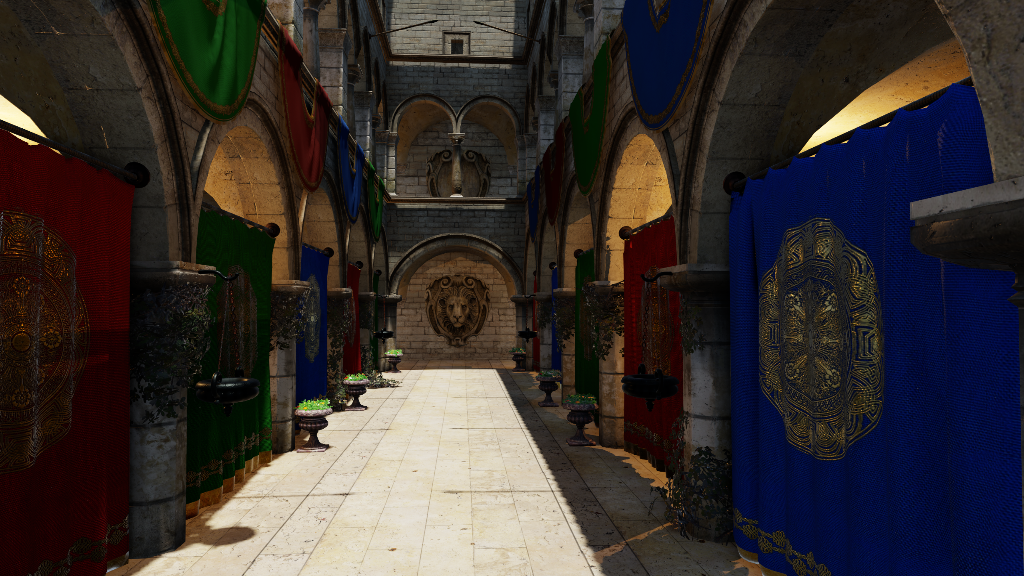
\includegraphics[width=0.48\textwidth]{figures/ss_all.png}\hfill%
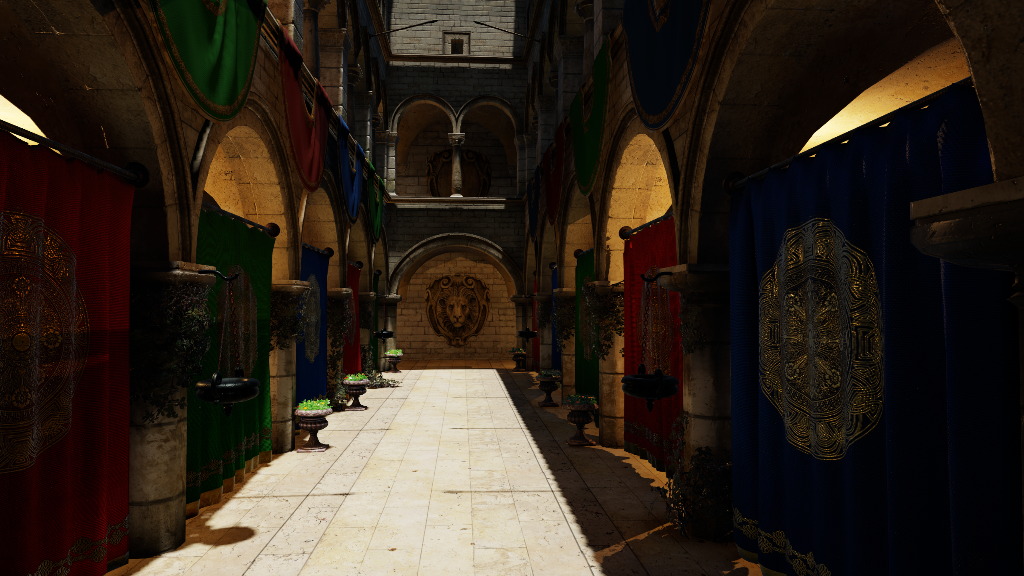
\includegraphics[width=0.48\textwidth]{figures/rt_all.png}
\caption[Screen-space naspram ray-traced konfiguracije]{Ista scena i kamera, dve celovite
konfiguracije: screen-space (levo: mapa senki, SSAO, SSR, SSGI) naspram ray-traced (desno: trasirane
senke, RTAO, RT refleksije, RT GI). Senke prate ostatak jer screen-space nema svoj pandan trasiranoj
senci, pa je mapa ono \v{s}to ta familija zaista koristi; to je ista podela koju koristi i red
\rqt{sve RT} u Tabeli~\ref{tab:quality}. Screen-space varijanta je svetlija jer ne mo\v{z}e da oduzme
svetlo koje dolazi od geometrije van ekrana.}
\label{fig:rt-vs-ss}
\end{figure}

\begin{figure}[tbp]
\centering
\begin{minipage}{0.48\textwidth}\centering
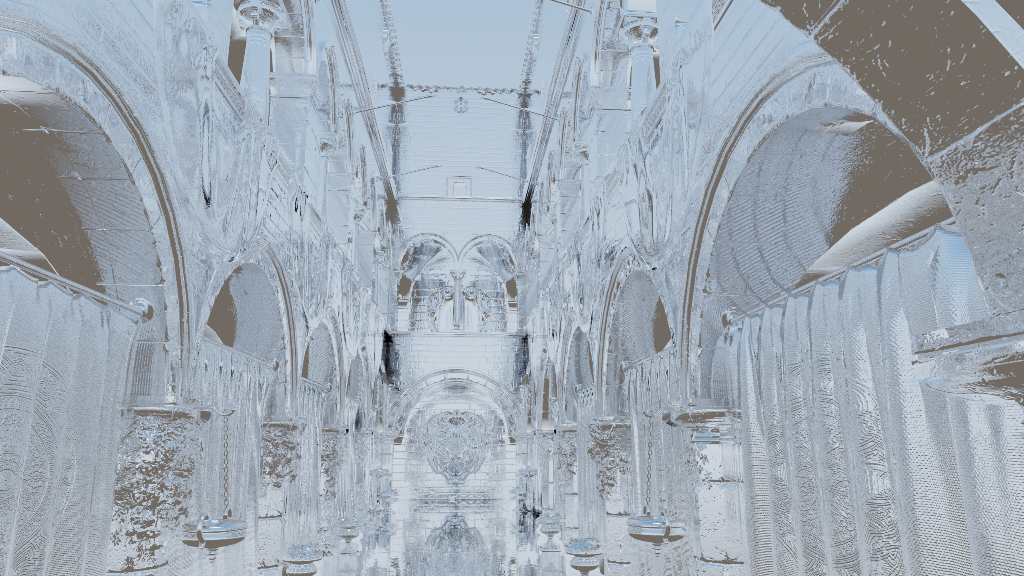
\includegraphics[width=\linewidth]{figures/ssvsrt_ssr.png}\\{\small SSR}
\end{minipage}\hfill
\begin{minipage}{0.48\textwidth}\centering
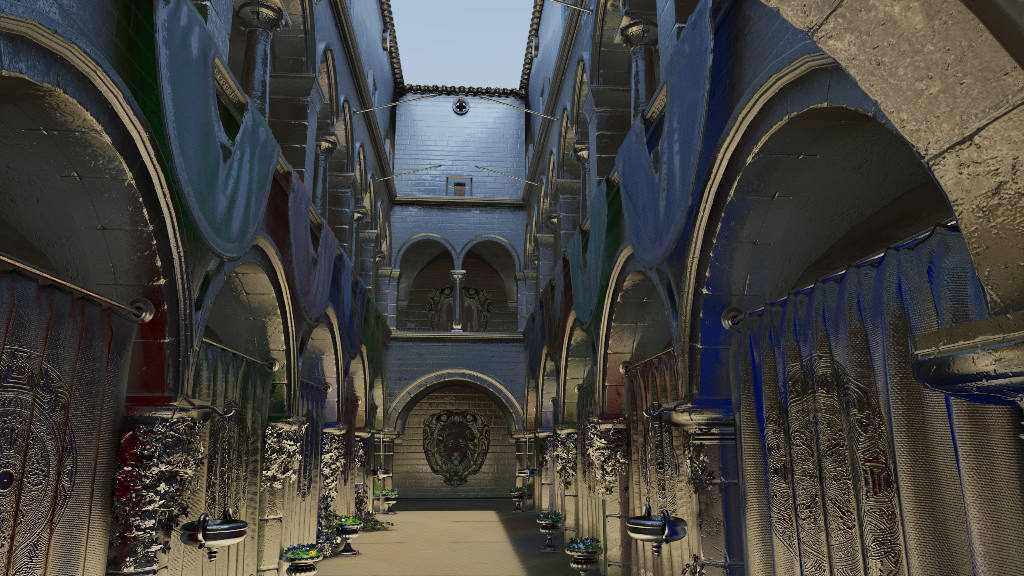
\includegraphics[width=\linewidth]{figures/ssvsrt_rtrefl.png}\\{\small RT refleksije}
\end{minipage}
\caption[Sirov bafer refleksije: SSR naspram RT]{Sirov bafer refleksije (\texttt{render.debugview} 3),
isti pogled i iste podrazumevane vrednosti; SSR i RT pi\v{s}u u isti bafer, pa je jedina promenljiva
izvor refleksije. Kada mar\v{s} kroz dubinski bafer ne na\dj e ni\v{s}ta, SSR vra\'ca prefiltriranu
mapu okru\v{z}enja: 9.0\% piksela je zbog toga skoro belo, naspram 0.0\% na desnoj strani, a srednja
vrednost bafera je 169.4 naspram 65.99. U slo\v{z}enom kadru se ta razlika gubi ispod direktnog
osvetljenja, zbog \v{c}ega je FLIP dve tehnike gotovo isti.}
\label{fig:ssvsrt-refl}
\end{figure}

\section{Stabilnost pod kretanjem}
\label{sec:motion}

Every quality figure so far comes from a static camera, which Section~\ref{sec:denoise-eval} found
hides most of what the spatial denoiser does: it cuts frame-to-frame flicker by \flickerPct\% while
moving the static metrics by less than measurement noise, an argument made there only by proxy. This
section moves the camera.

Flying a fixed route, capturing frames along it and scoring each against a converged path trace of
the same instant produces a caution about the method before any fact about the renderer: across the
eleven techniques, the per-frame FLIP measured this way correlates with the static FLIP of
Section~\ref{sec:poredjenje} at $r = +0.99$, very nearly the same measurement taken twice. A
converged per-frame path trace is a sequence of independent still images with no temporal structure,
since nothing in its construction relates one frame to the next, so error measured against it has no
temporal component to carry however much the camera moves. The defect is in that experimental design
rather than in the implementation, and it is a known conflation: k-DOP Clipping
\cite{ikkala2024kdop} states outright that a supersampled reference introduces a constant error by
also comparing general temporal-antialiasing quality against supersampling. The canonical denoiser
papers avoid it by reporting accuracy against a reference and temporal behaviour separately, the
latter with a reference-free measure.

Two quantities in the moving capture do carry information the static gate cannot. The first compares
how much the technique changes between consecutive frames against how much the \emph{reference}
changes over the same interval, so that motion inherent to the scene is subtracted and only excess
instability remains. Subtracting matters: on this route the reference itself moves by a FLIP of about
0.09 between adjacent frames, which a naive frame difference would report as instability. Ranked by
it (Table~\ref{tab:motion}), the techniques order exactly as the flicker proxy predicted, the fully
reconstructed configurations most stable and plain rasterization least, which is
Section~\ref{sec:denoise-eval}'s conclusion reached under motion instead of by proxy: the spatial
filter buys stability rather than static fidelity. The two temporal metrics disagree usefully:
\texttt{rtgi} has the best tFLIP while \texttt{all-rt} has the best JOD, because tFLIP isolates
temporal excess alone where ColorVideoVDP is spatio-temporal and \texttt{all-rt} is far more accurate
spatially.

\begin{table}[tbp]
\caption[Stabilnost pod kretanjem po tehnici]{Stabilnost pod kretanjem, prosek preko \v{c}etiri probne
ta\v{c}ke rute (RX 9070 XT), pore\dj ano po FLIP-u. tFLIP meri koliko se tehnika menja izme\dj u
susednih kadrova preko onoga koliko se menja sama referenca; ka\v{s}njenje je pokretni kadar naspram
sopstvenog konvergiranog mirnog kadra u istoj pozi. JOD je ColorVideoVDP, jedina mera ovde koja
direktno modeluje vremensku osetljivost.}
\label{tab:motion}
\centering
\begin{tabular}{lrrrr}
\toprule
Tehnika & FLIP $\downarrow$ & tFLIP $\downarrow$ & ka\v{s}njenje $\downarrow$ & JOD $\uparrow$ \\
\midrule
sve RT (all-RT)                  & 0.173 & 0.0082 & 0.104 & 4.81 \\
RT GI                            & 0.208 & 0.0081 & 0.119 & 3.89 \\
SSGI                             & 0.293 & 0.0161 & 0.129 & 3.28 \\
stohasti\v{c}ke senke (bez spec.) & 0.328 & 0.0120 & 0.126 & 3.18 \\
RT senke                         & 0.329 & 0.0154 & 0.120 & 3.22 \\
stohasti\v{c}ke senke            & 0.330 & 0.0127 & 0.127 & 3.16 \\
RT AO                            & 0.343 & 0.0198 & 0.124 & 3.25 \\
SSAO                             & 0.346 & 0.0198 & 0.123 & 3.16 \\
RT refleksije                    & 0.347 & 0.0162 & 0.120 & 3.17 \\
SSR                              & 0.362 & 0.0203 & 0.125 & 3.09 \\
raster                           & 0.362 & 0.0205 & 0.124 & 3.05 \\
\bottomrule
\end{tabular}

\end{table}

The second is lag: the moving frame scored against this renderer's own converged still at the same
pose, which measures how far reconstruction trails the camera, read across the route in
Table~\ref{tab:motion-probes} for the two ends of the ranking. Velocity reversal is the costliest
motion, and not because of speed, since the route holds translation essentially constant: what is
special about a reversal is that the velocity vector changes sign, the documented pathological case
for history rejection. The parked probe is an order of magnitude below the moving ones and acts as
the control that makes them readable.

\begin{table}[tbp]
\caption[Stabilnost i ka\v{s}njenje po ta\v{c}ki rute]{Iste dve vremenske mere razlo\v{z}ene po
probnim ta\v{c}kama, za krajeve rangiranja. Vrednosti se ne porede izme\dj u kolona: svaka ta\v{c}ka
gleda drugi sadr\v{z}aj, pa je razlika me\dj u njima uglavnom razlika u onome \v{s}to je na ekranu.}
\label{tab:motion-probes}
\centering
\begin{tabular}{llrrrr}
\toprule
Technique & metric & dolly & strafe & reversal & parked \\
\midrule
raster & tFLIP & 0.0193 & 0.0319 & 0.0270 & 0.0036 \\
raster & lag & 0.120 & 0.175 & 0.185 & 0.016 \\
all RT (all-RT) & tFLIP & 0.0137 & 0.0161 & 0.0010 & 0.0019 \\
all RT (all-RT) & lag & 0.089 & 0.138 & 0.166 & 0.024 \\
\bottomrule
\end{tabular}

\end{table}

Three cautions belong with these numbers. They must not be compared across probes as if the probes
were equally hard, because each looks at different scene content: plain rasterization scores its
\emph{best} per-frame FLIP on the reversal probe while showing its worst lag there. The lag measure is
this renderer against its own still, so it can be driven to zero by degrading the still and must never
be used as an optimisation target. And its absolute scale depends on the capture protocol, which was
corrected during this work, so only figures from the current baselines may be quoted and never mixed
with earlier ones.

\section{Kvalitet izme\dj u proizvo\dj a\v{c}a}
\label{sec:cross-vendor-quality}

The cross-vendor argument rests on the two adapters running identical code, which elsewhere justifies
comparing \emph{time}. If the reconstructed images did not also agree, a timing difference could
always be dismissed as the two cards having done different amounts of work.

The whole quality matrix was captured a second time on the RTX 5070, giving 33 viewpoint and technique
pairs. Across all 33 the largest absolute difference in FLIP between the adapters is \textbf{0.0037},
the median is \textbf{0.0007}, and 24 of the 33 fall below 0.001. The secondary metrics agree to the
same degree: PSNR never differs by more than 0.10 dB and SSIM never by more than 0.0045. For scale,
the difference this chapter is actually interested in, between raster and all effects enabled, is a
FLIP of \qRasterFlip{} against \qAllRtFlip{}, two orders of magnitude larger than the vendor
disagreement.

Technique quality is therefore effectively vendor-independent here, so the entire
cross-vendor story of this thesis is cost rather than image quality:
the per-effect timings in Section~\ref{sec:cena} and the shadow-strategy inversion in
Section~\ref{sec:analiza-shadow-strategy} can be read as pure performance differences, with no
accompanying quality caveat.

Both adapters are scored against the \emph{same} path-traced reference, and the obvious alternative
would have destroyed the result. The
reference cache is keyed on the scene, the camera pose, the frame count and the content of the
path-tracing shaders, and deliberately not on the device, so the second adapter reuses the reference
the first produced rather than tracing its own. Had each been scored against a reference it produced
itself, every comparison would have carried the difference between two independently converged path
traces, and there is no reason to assume that difference is small next to the technique difference
being measured. Sharing the reference makes the reference error common to both sides, where it
cancels.

Two limits bound the claim. The residual disagreement is not zero, and the largest of it sits on the
ambient-occlusion and shadow rows, which are also the effects whose rays interact with the cutout
geometry where the two drivers genuinely differ (Section~\ref{sec:metodologija}). That is consistent
with the opacity-micromap disparity being the mechanism, although this experiment does not isolate it.
And the reference is shared here because both adapters were measured on one machine with a warm cache;
on two machines each would trace its own, and the comparison would require transferring the reference
rather than recomputing it.

\section{Zauzetost i cena \v{s}ejdera}
\label{sec:occupancy}

Static shader occupancy, how many registers each ray-tracing and denoising shader needs and how many
waves the hardware can therefore keep in flight, is the one place where the two vendors compare on
something other than time, and it explains part of the cost difference the rest of the chapter
measures.

Two artifacts feed it, with deliberately different authority. For AMD the offline analyser compiles
every shader and permutation, so its coverage is complete and deterministic, and it is what the
project gates on. For NVIDIA no offline analyser exists, since register allocation happens inside the
driver's just-in-time compiler, so those figures are read back from the driver through
\texttt{VK\_KHR\_pipeline\_executable\_properties} after the pipelines are built. The two agree on
every AMD register count they share, which is what licenses carrying the offline permutation labels
over to the runtime numbers: the runtime capture reports both \texttt{DefaultLit} variants under one
pipeline name and cannot tell them apart on its own.

\begin{table}[tbp]
\caption{Registri i teorijska zauzetost klju\v{c}nih \v{s}ejdera na oba GPU-a. Za AMD: broj VGPR-a i
najve\'ci mogu\'ci broj wave32 talasa po SIMD-u (1536 VGPR-a, granularnost 24, najvi\v{s}e 16). Za
NVIDIA: broj registara po niti i najve\'ci broj warp-ova po SM-u (65536 registara, najvi\v{s}e 48).
Obe vrednosti su teorijske i izvedene iz broja registara, ne izmerene profajlerom. Generi\v{s}e se iz
committovanih baseline-a skriptom \texttt{tools/gen\_shader\_tables.py}.}
\label{tab:occupancy}
\centering
\begin{tabular}{lrrrr}
\toprule
& \multicolumn{2}{c}{RX 9070 XT (RDNA4)} & \multicolumn{2}{c}{RTX 5070 (Blackwell)} \\
\cmidrule(lr){2-3}\cmidrule(lr){4-5}
\v{S}ejder & VGPR & talasa/SIMD & registara & warp-ova/SM \\
\midrule
\texttt{DefaultLit.frag} (inline senke) & 127 & 10/16 & 80 & 25/48 \\
\texttt{DefaultLit.frag} (bez inline senki) & 87 & 16/16 & 64 & 32/48 \\
\texttt{GI.comp} & 83 & 16/16 & 64 & 32/48 \\
\texttt{Reflection.comp} & 81 & 16/16 & 64 & 32/48 \\
\texttt{AO.comp} & 60 & 16/16 & 48 & 42/48 \\
\texttt{GIDenoise.comp} (GI) & 59 & 16/16 & 48 & 42/48 \\
\bottomrule
\end{tabular}

\end{table}

Only one shader on the render path is occupancy-limited on either card, and it is the same one:
\texttt{DefaultLit.frag} in its inline-shadow permutation, at 127 VGPRs and 10 of 16 waves on the
9070 XT. Compiled without the inline shadow query it drops to 87 VGPRs and full occupancy, which
locates the cost precisely: tracing shadow rays inside the forward shader is what pushes it over a
wave boundary, the same effect Section~\ref{sec:cena} sees as a Forward pass that grows by 3.482 ms.
Nothing in the table spills registers, and across all 47 cooked shaders exactly one uses scratch
memory at all (\texttt{NeuralConv.comp}, 272 bytes), off the render path.

Figure~\ref{fig:occupancy-cliff} plots why the two permutations land so far apart for a difference of
40 registers. Occupancy is a step function of register use, since registers are allocated in fixed
blocks of 24 on this architecture and the wave count is the register file divided by that rounded-up
allocation. Between 24 and 96 VGPRs every shader gets all 16 waves, so the five shaders in the flat
region differ in register use by a factor of 1.5 (59 to 87) at no cost in parallelism. Past 96 the
count falls in steps: the inline-shadow permutation at 127 VGPRs allocates 144 and gets 10 waves; had
it stayed at or below 96, as its non-tracing sibling does at 87, it would have cost nothing. Hence gating
on occupancy rather than on the register count directly, and acting on a register increase only when
it crosses a step.

\begin{figure}[tbp]
\centering
\begin{tikzpicture}
\begin{axis}[width=0.86\textwidth, height=6.2cm,
  xlabel={VGPR-a po niti}, ylabel={talasa po SIMD-u (wave32)},
  xmin=24, xmax=192, ymin=0, ymax=17.5,
  ytick={0,4,8,12,16}, xtick={24,48,72,96,120,144,168,192},
  grid=major, grid style={black!12}, tick label style={font=\small},
  label style={font=\small}]
  \addplot[const plot, thick, black] table[col sep=tab, x=vgpr, y=waves] {data/occupancy-curve.dat};
  \addplot[only marks, mark=*, mark size=1.9pt, black]
    table[col sep=tab, x=vgpr, y=waves] {data/occupancy-marks.dat};
  \node[font=\footnotesize, anchor=west] at (axis cs:130,10.9) {\texttt{DefaultLit} (inline senke)};
  \node[font=\footnotesize, anchor=east] (nobez) at (axis cs:80,13.6) {\texttt{DefaultLit} (bez)};
  \draw[black!55, thin] (nobez.east) -- (axis cs:87,15.6);
\end{axis}
\end{tikzpicture}
\caption[Zauzetost kao stepenasta funkcija broja VGPR-a]{Teorijska zauzetost kao stepenasta funkcija broja VGPR-a na RDNA4 (1536 VGPR-a,
granularnost 24, najvi\v{s}e 16 talasa). Ta\v{c}ke su \v{s}ejderi iz Tabele~\ref{tab:occupancy}. Do 96
VGPR-a razlika u broju registara ne ko\v{s}ta ni\v{s}ta; \texttt{DefaultLit} sa inline senkama pada
preko granice na 127.}
\label{fig:occupancy-cliff}
\end{figure}

The cross-vendor comparison inverts the naive reading. NVIDIA uses markedly fewer registers for the
same shader, 80 against 127 for the inline-shadow variant, yet its relative occupancy is \emph{lower},
25 of 48 warps against 10 of 16 waves (52\% against 62\%), because of the ratio each architecture
provides: a Blackwell SM has 65536 registers for up to 48 warps of 32 threads, about 42 registers per
thread at full occupancy, so pressure begins to bite earlier there than the raw counts suggest. Fewer
registers used does not mean more parallelism available.

Three limits belong with these numbers. The occupancy is theoretical and register-derived, so it is an
upper bound on both vendors and says nothing about what is achieved once memory stalls and other
limits are included; that needs a runtime profiler. The RDNA4 register allocation granularity is taken
from documentation and has not been confirmed against a per-compile report the way the RDNA3 figure
was, so a wave count sitting near a boundary is model-dependent: at a granularity of 8 rather than 24
the inline-shadow permutation would read 12 of 16 rather than 10. And the NVIDIA figure is explicitly
an upper bound, since the allocation granularity for that compute capability is not published and
rounding up can only lower the warp count.

Register spilling on NVIDIA is deliberately not reported: the driver returns a \texttt{Local Memory
Size} whose upper 32 bits are a constant, so the values differ only in their low half, and while that
low half is very likely the real figure, masking it would be inference presented as measurement.

\chapter{Zaklju\v{c}ak}
\label{ch:zakljucak}


\section{Rezime (osvrt na ciljeve iz zadatka)}

The goal set in the assignment was to implement four ray-traced lighting effects, shadows, ambient
occlusion, reflections, and diffuse global illumination, through inline ray queries in a custom
Vulkan engine, and to characterize the cost and quality of each. All four effects were implemented as
described in Chapter~\ref{ch:implementacija}, sharing one hit-shading routine over a bindless geometry
table and one reusable SVGF denoiser, and integrated into an existing rasterizing forward renderer
rather than a standalone tracer. The evaluation in Chapter~\ref{ch:analiza} isolates the per-effect
GPU cost with an A/B benchmark and measures reconstruction quality against a converged path-traced
reference, and compares the identical pipeline
across two GPU vendors (AMD RDNA4 and NVIDIA Blackwell).
The headline numbers are collected in Table~\ref{tab:summary}. The two cards do not agree on which
effect costs most: on the RX 9070 XT shadows dominate, while on the RTX 5070 shadows, reflections and
global illumination sit within \perfNVSpread{} ms of one another, which is inside the run-to-run
spread, so on that card they are indistinguishable in cost.

\begin{table}[tbp]
\caption[Sa\v{z}etak izmerenih rezultata]{Sa\v{z}etak izmerenih rezultata. Cena po efektu je razlika
ukupnog GPU vremena izme\dj u susednih konfiguracija; kvalitet je prosek preko tri pogleda naspram
konvergirane path-traced reference na RX 9070 XT.}
\label{tab:summary}
\centering
\begin{tabular}{lrr}
\toprule
 & RX 9070 XT & RTX 5070 \\
\midrule
osnova bez RT (ms)      & \perfBaseAMD{}        & \perfBaseNV{} \\
senke (ms)              & \perfEffShadowsAMD{}  & \perfEffShadowsNV{} \\
AO (ms)                 & \perfEffAoAMD{}       & \perfEffAoNV{} \\
refleksije (ms)         & \perfEffReflAMD{}     & \perfEffReflNV{} \\
GI (ms)                 & \perfEffGiAMD{}       & \perfEffGiNV{} \\
\midrule
ukupno, sva \v{c}etiri (ms) & \perfTotalAMD{}   & \perfTotalNV{} \\
\midrule
FLIP: raster $\rightarrow$ sve RT  & \multicolumn{2}{c}{\qRasterFlip{} $\rightarrow$ \qAllRtFlip{}} \\
PSNR (dB): raster $\rightarrow$ sve RT & \multicolumn{2}{c}{\qRasterPsnr{} $\rightarrow$ \qAllRtPsnr{}} \\
SSIM: raster $\rightarrow$ sve RT  & \multicolumn{2}{c}{\qRasterSsim{} $\rightarrow$ \qAllRtSsim{}} \\
\bottomrule
\end{tabular}
\end{table}

Two of the sweeps sharpen that picture. The ray-count knee sits at one ray per pixel: going from one
to eight rays costs \rcGpuPct\% more GPU time for a \rcPsnrGain{} dB PSNR gain, because the denoiser and temporal
accumulation already recover most of the achievable quality from a single sample
(Section~\ref{sec:raycount}). The spatial denoiser's own contribution is likewise not where a static
metric can see it: it moves PSNR, SSIM and FLIP by less than run-to-run noise, while cutting
frame-to-frame RMS on a static view from \flickerOff{} to \flickerOn{}, a \flickerPct\% reduction, for \perfDenoiseAMD{} ms
(Section~\ref{sec:denoise-eval}). The honest reading is that at this sample count the temporal history
does the reconstruction and the spatial filter buys stability rather than static fidelity.

The practical value is a demonstration that a hybrid
ray-query pipeline gives correct off-screen lighting at an interactive budget without a full path
tracer, which is directly applicable to real-time engines that want physically grounded indirect
lighting, contact shadows, and reflections.

\section{Ograni\v{c}enja}

The work has clear limitations, stating them sharpens what the results do and do not show. The
measurements are taken on two GPUs of comparable market tier and a single scene class, so the absolute numbers do not
generalize across hardware or content. Global illumination is limited to a single diffuse bounce, and
shadows are hard or lightly softened rather than physically accurate area shadows. To stay within a
real-time budget the ray counts are kept very low (one or two per pixel), which places heavy demand
on the denoiser and exposes its failure modes: temporal ghosting and lag under fast motion,
particularly for reflections, which reuse the diffuse-tuned temporal reprojection. The
top-level acceleration structure is fully rebuilt on every dynamic frame rather than refit, which is
heavier than necessary for small transform changes. Finally, using inline ray queries
gives up the hardware ray scheduling and recursion that a ray-tracing pipeline would provide, a
deliberate tradeoff for integration simplicity that would matter for deeper or more numerous bounces.

\section{Budu\'ci rad}

Several directions extend the work. Sampling is the most immediate: replacing the naive per-light and
cosine-hemisphere sampling with reservoir resampling (ReSTIR and ReSTIR GI) would improve quality at
equal ray count, especially for many lights and for indirect paths
\cite{bitterli2020restir, ouyang2021restirgi}. Reconstruction is the second: the engine already
contains a temporal neural network used as an anti-aliasing resolve, and a natural next step is a
learned denoiser or upscaler replacing or augmenting SVGF, together with the vendor-neutral,
cross-vendor cooperative-matrix inference study that motivated an earlier version of this project. A
third direction is scaling the denoised shadows to many lights more cheaply, with a MegaLights-style
stochastic per-pixel light selection on the shared denoiser, rather than tracing every light every
frame; a dedicated, penumbra-aware shadow denoiser in place of the shared one is a related refinement. Finally, the cross-vendor comparison here covers two current-generation cards; broadening it to more cards and
older generations, plus a second rendering backend (DirectX 12), would extend the performance story further.


% Manual bibliography, hand-formatted to PPK's citation style, ordered by citation.
\clearpage
\phantomsection
\addcontentsline{toc}{chapter}{\bibname}
% Bibliography in PPK format (Surname Name, \rqt{Title}, edition/venue, publisher, place, year),
% ordered by citation. Hand-formatted; this list is the only bibliography, there is no BibTeX step.
\begin{thebibliography}{99}

\bibitem{mittring2007cryengine}
Mittring Martin, \rqt{Finding Next Gen: CryEngine 2}, SIGGRAPH Courses, 2007.

\bibitem{bavoil2008hbao}
Bavoil Louis, Sainz Miguel, Dimitrov Rouslan, \rqt{Image-Space Horizon-Based Ambient Occlusion},
SIGGRAPH Talks, 2008.

\bibitem{crassin2011vxgi}
Crassin Cyril, Neyret Fabrice, Sainz Miguel, Green Simon, Eisemann Elmar, \rqt{Interactive Indirect
Illumination Using Voxel Cone Tracing}, Computer Graphics Forum (Pacific Graphics), 2011.

\bibitem{kajiya1986rendering}
Kajiya James T., \rqt{The Rendering Equation}, SIGGRAPH, 1986.

\bibitem{schied2017svgf}
Schied Christoph, Kaplanyan Anton, Wyman Chris, Patney Anjul, Chaitanya Chakravarty R. Alla, Burgess
John, Liu Shiqiu, Dachsbacher Carsten, Lefohn Aaron, Salvi Marco, \rqt{Spatiotemporal Variance-Guided
Filtering: Real-Time Reconstruction for Path-Traced Global Illumination}, High Performance Graphics
(HPG), 2017.

\bibitem{moller1997raytri}
M\"oller Tomas, Trumbore Ben, \rqt{Fast, Minimum Storage Ray/Triangle Intersection}, Journal of
Graphics Tools, 1997.

\bibitem{pharr2016pbrt}
Pharr Matt, Jakob Wenzel, Humphreys Greg, \rqt{Physically Based Rendering: From Theory to
Implementation}, 3rd ed., Morgan Kaufmann, 2016.

\bibitem{akenine2018rtr}
Akenine-M\"oller Tomas, Haines Eric, Hoffman Naty, Pesce Angelo, Iwanicki Micha\l{}, Hillaire
S\'ebastien, \rqt{Real-Time Rendering}, 4th ed., A K Peters/CRC Press, 2018.

\bibitem{khronos_rayquery}
The Khronos Group, \rqt{Vulkan Specification: \texttt{VK_KHR_ray_query},
\texttt{VK_KHR_acceleration_structure}}, \url{https://registry.khronos.org/vulkan/}, accessed 2026.

\bibitem{majercik2019ddgi}
Majercik Zander, Guertin Jean-Philippe, Nowrouzezahrai Derek, McGuire Morgan, \rqt{Dynamic Diffuse
Global Illumination with Ray-Traced Irradiance Fields}, Journal of Computer Graphics Techniques
(JCGT), 2019.

\bibitem{nvidia_rtxgi}
NVIDIA, \rqt{RTX Global Illumination (RTXGI)}, \url{https://developer.nvidia.com/rtxgi}, accessed
2026.

\bibitem{epic_lumen}
Epic Games, \rqt{Lumen Global Illumination and Reflections}, Unreal Engine Documentation,
\url{https://docs.unrealengine.com/}, accessed 2026.

\bibitem{bitterli2020restir}
Bitterli Benedikt, Wyman Chris, Pharr Matt, Shirley Peter, Lefohn Aaron, Jarosz Wojciech,
\rqt{Spatiotemporal Reservoir Resampling for Real-Time Ray Tracing with Dynamic Direct Lighting}, ACM
Transactions on Graphics (SIGGRAPH), 2020.

\bibitem{ouyang2021restirgi}
Ouyang Y., Liu S., Kettunen M., Pharr M., Pantaleoni J., \rqt{ReSTIR GI: Path Resampling for
Real-Time Path Tracing}, Computer Graphics Forum (HPG), 2021.

\bibitem{schied2018asvgf}
Schied Christoph, Peters Christoph, Dachsbacher Carsten, \rqt{Gradient Estimation for Real-Time
Adaptive Temporal Filtering}, ACM on Computer Graphics and Interactive Techniques (HPG), 2018.

\bibitem{nvidia_nrd}
NVIDIA, \rqt{Real-Time Denoisers (NRD)},
\url{https://developer.nvidia.com/rtx/ray-tracing/rt-denoisers}, accessed 2026.

\bibitem{intel_oidn}
Intel, \rqt{Open Image Denoise (OIDN)}, \url{https://www.openimagedenoise.org/}, accessed 2026.

\bibitem{karis2014taa}
Karis Brian, \rqt{High Quality Temporal Supersampling}, SIGGRAPH Courses: Advances in Real-Time
Rendering in Games, 2014.

\bibitem{ikkala2024kdop}
Ikkala Joel, Aittala Miika, Laine Samuli, Lehtinen Jaakko, \rqt{k-DOP Clipping: Robust Temporal
Antialiasing}, SIGGRAPH Asia, 2024.

\bibitem{amd_rdna_isa}
Advanced Micro Devices, \rqt{RDNA3 / RDNA4 Instruction Set Architecture Reference Guide},
\url{https://gpuopen.com/amd-gpu-architecture-programming-documentation/}, accessed 2026.

\bibitem{nvidia_turing}
NVIDIA Corporation, \rqt{NVIDIA Turing GPU Architecture Whitepaper}, WP-09183-001, 2018.

\bibitem{nvidia_ada}
NVIDIA Corporation, \rqt{NVIDIA Ada GPU Architecture Whitepaper}, V2.01, 2022.

\bibitem{andersson2020flip}
Andersson Pontus, Nilsson Jim, Akenine-M\"oller Tomas, Oskarsson Magnus, \r{A}str\"om Kalle, Fairchild
Mark D., \rqt{FLIP: A Difference Evaluator for Alternating Images}, Proceedings of the ACM on Computer
Graphics and Interactive Techniques (High Performance Graphics), 2020.

\bibitem{wang2004ssim}
Wang Zhou, Bovik Alan C., Sheikh Hamid R., Simoncelli Eero P., \rqt{Image Quality Assessment: From
Error Visibility to Structural Similarity}, IEEE Transactions on Image Processing, 2004.

\bibitem{mantiuk2024cvvdp}
Mantiuk Rafa\l{} K., Hanji Param, Ashraf Maliha, Asano Yuta, Chapiro Alexandre,
\rqt{ColorVideoVDP: A Visual Difference Predictor for Image, Video and Display Distortions}, ACM
Transactions on Graphics (SIGGRAPH), 2024.

\bibitem{chu2020tecogan}
Chu Mengyu, Xie You, Mayer Jonas, Leal-Taix\'e Laura, Thuerey Nils, \rqt{Learning Temporal Coherence
via Self-Supervision for GAN-based Video Generation}, ACM Transactions on Graphics (SIGGRAPH), 2020.

\bibitem{koskela2019bmfr}
Koskela Matias, Immonen Kalle, M\"akitalo Markku, Foi Alessandro, Viitanen Timo, J\"a\"askel\"ainen
Pekka, Kultala Heikki, Takala Jarmo, \rqt{Blockwise Multi-Order Feature Regression for Real-Time
Path-Tracing Reconstruction}, ACM Transactions on Graphics, 2019.

\bibitem{talbot2005ris}
Talbot Justin F., Cline David, Egbert Parris, \rqt{Importance Resampling for Global Illumination},
Eurographics Symposium on Rendering (EGSR), 2005.

\bibitem{wolfe2022stbn}
Wolfe Alan, Morrical Nathan, Akenine-M\"oller Tomas, Ramamoorthi Ravi, \rqt{Spatiotemporal Blue Noise
Masks}, Eurographics Symposium on Rendering (EGSR), 2022.

\bibitem{epic_megalights}
Epic Games, \rqt{MegaLights}, Unreal Engine Documentation,
\url{https://dev.epicgames.com/documentation/en-us/unreal-engine/megalights-in-unreal-engine},
accessed 2026.

\bibitem{itu_p910}
International Telecommunication Union, \rqt{ITU-T Recommendation P.910: Subjective Video Quality
Assessment Methods for Multimedia Applications}, 2023.

\end{thebibliography}


\end{document}
